\documentclass[11pt]{article}

% ============================================================
% COPY FAIL -- TECHNICAL SECURITY RESEARCH REPORT
% CVE-2026-31431
%
% OUTPUT MODE
%   \PrintWrapfalse -> complete A4 report with front and back cover
%   \PrintWraptrue  -> one-page print wrap: back | spine | front
% ============================================================

\newif\ifPrintWrap
\PrintWrapfalse

% The report contains 146 interior pages (73 sheets). Keep this value at
% 8 mm only as a layout preview; replace it with the exact spine width
% supplied by the printer for the selected paper before final production.
\newlength{\SpineWidth}
\setlength{\SpineWidth}{8mm}
\newlength{\CoverBleed}
\setlength{\CoverBleed}{3mm}
\newlength{\TrimWidth}
\setlength{\TrimWidth}{210mm}
\newlength{\TrimHeight}
\setlength{\TrimHeight}{297mm}
\newlength{\WrapWidth}
\setlength{\WrapWidth}{\dimexpr 2\TrimWidth+\SpineWidth+2\CoverBleed\relax}
\newlength{\WrapHeight}
\setlength{\WrapHeight}{\dimexpr \TrimHeight+2\CoverBleed\relax}

% Frozen project metadata. Never replace \ReportDate with \today.
\newcommand{\ReportDate}{September 8, 2026}
\newcommand{\ReportDateISO}{2026.09.08}

% ------------------------------------------------------------
% Encoding and language
% ------------------------------------------------------------

\usepackage[T1]{fontenc}
\usepackage[utf8]{inputenc}
\usepackage[english]{babel}

% ------------------------------------------------------------
% Typography
% ------------------------------------------------------------

\usepackage{lmodern}
\usepackage{microtype}
\usepackage{tocloft}
\usepackage{parskip}
\usepackage[scaled=0.94]{helvet}
\setlength{\parindent}{0pt}
\setlength{\parskip}{0.7em}
\raggedbottom
\clubpenalty=10000
\widowpenalty=10000
\displaywidowpenalty=10000
\emergencystretch=2em

\newcommand{\displayfont}{\sffamily}

% ------------------------------------------------------------
% Page layout
% ------------------------------------------------------------

\ifPrintWrap
  \usepackage[
    paperwidth=\WrapWidth,
    paperheight=\WrapHeight,
    margin=0pt
  ]{geometry}
\else
  \usepackage[
    a4paper,
    top=2.5cm,
    bottom=2.6cm,
    left=2.7cm,
    right=2.7cm
  ]{geometry}
\fi

% ------------------------------------------------------------
% Colour palette
% ------------------------------------------------------------

\usepackage[table]{xcolor}
\definecolor{MoriPurple}{HTML}{9D4DFF}
\definecolor{MoriElectric}{HTML}{7C20FF}
\definecolor{MoriDeepPurple}{HTML}{6D2CC4}
\definecolor{MoriLavender}{HTML}{C9C2D6}
\definecolor{MoriMist}{HTML}{F4F0FF}
\definecolor{MoriGray}{HTML}{9E9E9E}
\definecolor{MoriInk}{HTML}{18171C}
\definecolor{MoriPaper}{HTML}{FFFFFF}
\definecolor{MoriNight}{HTML}{100F14}
\definecolor{MoriNightSoft}{HTML}{15131B}
\definecolor{MoriPanel}{HTML}{24212B}
\definecolor{MoriCode}{HTML}{F6F4F8}
\definecolor{MoriRule}{HTML}{DCD6E4}
\definecolor{MoriMuted}{HTML}{68636F}
\color{MoriInk}

% ------------------------------------------------------------
% Core packages
% ------------------------------------------------------------

\usepackage{graphicx}
\usepackage{booktabs}
\usepackage{caption}
\usepackage{float}
\usepackage{tabularx}
\usepackage{array}
\usepackage{tikz}
\usetikzlibrary{calc}
\usepackage{enumitem}
\usepackage{listings}
\usepackage[most]{tcolorbox}

% ------------------------------------------------------------
% Section styling
% ------------------------------------------------------------

\usepackage{titlesec}

\titleformat{\section}
  {\displayfont\Large\bfseries\color{MoriInk}}
  {\colorbox{MoriPurple}{%
    \makebox[2.15em][c]{\color{MoriPaper}\strut\thesection}%
  }}
  {0.8em}
  {}
  [\vspace{0.3em}\color{MoriRule}\titlerule]

\titleformat{\subsection}
  {\displayfont\large\bfseries\color{MoriInk}}
  {\color{MoriPurple}\thesubsection}
  {0.75em}
  {}

\titleformat{\subsubsection}
  {\displayfont\normalsize\bfseries\color{MoriInk}}
  {\color{MoriPurple}\thesubsubsection}
  {0.75em}
  {}

\titlespacing*{\section}{0pt}{2.6em}{1em}
\titlespacing*{\subsection}{0pt}{1.8em}{0.6em}
\titlespacing*{\subsubsection}{0pt}{1.4em}{0.4em}

\titleformat{name=\section,numberless}
  {\displayfont\Large\bfseries\color{MoriInk}}
  {}
  {0pt}
  {}
  [\vspace{0.3em}\color{MoriRule}\titlerule]

% ------------------------------------------------------------
% Header and footer
% ------------------------------------------------------------

\usepackage{fancyhdr}
\setlength{\headheight}{24pt}
\setlength{\headsep}{0.55cm}
\pagestyle{fancy}
\fancyhf{}
\fancyhead[L]{%
  \displayfont\footnotesize\bfseries
  \textcolor{MoriPurple}{COPY FAIL}
  \textcolor{MoriGray}{\enspace//\enspace}
  \textcolor{MoriMuted}{CVE-2026-31431}%
}
\fancyhead[R]{%
  \displayfont\footnotesize\color{MoriMuted}
  \nouppercase{\rightmark}%
}
\fancyfoot[L]{%
  \displayfont\scriptsize\color{MoriGray}
  CONTROLLED SECURITY RESEARCH
}
\fancyfoot[R]{%
  \displayfont\footnotesize\bfseries\color{MoriMuted}
  \thepage
}
\renewcommand{\sectionmark}[1]{\markright{#1}}
\renewcommand{\headrulewidth}{0.45pt}
\renewcommand{\headrule}{%
  \hbox to\headwidth{%
    \color{MoriRule}\leaders\hrule height \headrulewidth\hfill
  }%
}
\renewcommand{\footrulewidth}{0pt}

% ------------------------------------------------------------
% Figures, tables, and contents
% ------------------------------------------------------------

\captionsetup{
  font=small,
  labelfont={bf,color=MoriPurple},
  textfont={color=MoriInk}
}
\renewcommand{\arraystretch}{1.15}
\newcolumntype{Y}{>{\raggedright\arraybackslash}X}

\renewcommand{\cfttoctitlefont}{%
  \displayfont\Huge\bfseries\color{MoriInk}%
}
\renewcommand{\cftaftertoctitle}{%
  \par\vspace{0.15em}%
  {\color{MoriRule}\hrule height 0.5pt}%
  \vspace{0.8em}%
}
\renewcommand{\cftsecfont}{\displayfont\bfseries\color{MoriInk}}
\renewcommand{\cftsecpagefont}{\displayfont\bfseries\color{MoriPurple}}
\renewcommand{\cftsubsecfont}{\displayfont\color{MoriMuted}}
\renewcommand{\cftsubsecpagefont}{\displayfont\color{MoriMuted}}
\renewcommand{\cftdotsep}{1.5}
\setlength{\cftbeforesecskip}{0.35em}
\setlength{\cftbeforesubsecskip}{0.08em}

% ------------------------------------------------------------
% Lists
% ------------------------------------------------------------

\setlist[itemize]{
  topsep=0.4em,
  itemsep=0.2em,
  parsep=0pt
}
\setlist[enumerate]{
  topsep=0.4em,
  itemsep=0.2em,
  parsep=0pt
}

% ------------------------------------------------------------
% Terminal and code blocks
% ------------------------------------------------------------

\lstdefinestyle{terminal}{
  backgroundcolor=\color{MoriCode},
  basicstyle=\ttfamily\footnotesize\color{MoriInk},
  frame=l,
  rulecolor=\color{MoriPurple},
  framerule=2.2pt,
  framesep=9pt,
  breaklines=true,
  breakatwhitespace=false,
  columns=fullflexible,
  keepspaces=true,
  showstringspaces=false,
  tabsize=4,
  xleftmargin=0.4em,
  xrightmargin=0.2em,
  framexleftmargin=0pt,
  aboveskip=1em,
  belowskip=1em,
  captionpos=b
}
\lstset{style=terminal}

% ------------------------------------------------------------
% Research callout boxes
% ------------------------------------------------------------

\tcbset{
  moribox/.style={
    enhanced,
    breakable,
    sharp corners,
    boxrule=0.45pt,
    colframe=MoriRule,
    colback=MoriMist,
    coltext=MoriInk,
    borderline west={2.6pt}{0pt}{MoriPurple},
    left=4mm,
    right=4mm,
    top=3mm,
    bottom=3mm,
    before skip=1em,
    after skip=1em
  }
}

\newtcolorbox{findingbox}{
  moribox,
  before upper={%
    \displayfont\scriptsize\bfseries\color{MoriPurple}
    FINDING\enspace//\par\smallskip
    \normalfont\normalsize\color{MoriInk}%
  }
}

\newtcolorbox{evidencebox}{
  moribox,
  borderline west={2pt}{0pt}{MoriLavender},
  before upper={%
    \displayfont\scriptsize\bfseries\color{MoriMuted}
    EVIDENCE\enspace//\par\smallskip
    \normalfont\normalsize\color{MoriInk}%
  }
}

\newtcolorbox{checkpointbox}{
  moribox,
  borderline west={3pt}{0pt}{MoriPurple},
  before upper={%
    \displayfont\scriptsize\bfseries\color{MoriPurple}
    CHECKPOINT\enspace//\par\smallskip
    \normalfont\normalsize\color{MoriInk}%
  }
}

\newtcolorbox{limitationbox}{
  moribox,
  colback=MoriCode,
  borderline west={2pt}{0pt}{MoriGray},
  before upper={%
    \displayfont\scriptsize\bfseries\color{MoriMuted}
    LIMITATION\enspace//\par\smallskip
    \normalfont\normalsize\color{MoriInk}%
  }
}

% ------------------------------------------------------------
% Hyperlinks and references
% ------------------------------------------------------------

\usepackage{hyperref}
\hypersetup{
  colorlinks=true,
  linkcolor=MoriPurple,
  citecolor=MoriPurple,
  urlcolor=MoriPurple,
  pdfborder={0 0 0},
  pdftitle={Copy Fail - CVE-2026-31431},
  pdfsubject={Technical Security Research Report},
  pdfauthor={Denis Krüger}
}
\usepackage[nameinlink,noabbrev]{cleveref}

% ------------------------------------------------------------
% Utility commands
% ------------------------------------------------------------

\newcommand{\code}[1]{%
  \begingroup
  \setlength{\fboxsep}{1.7pt}%
  \colorbox{MoriCode}{%
    \texttt{\small\color{MoriDeepPurple}\strut #1}%
  }%
  \endgroup
}

\newcommand{\statuspass}{%
  \raisebox{0.1ex}{\textcolor{MoriPurple}{\rule{1.05ex}{1.05ex}}}%
  \hspace{0.45em}%
  {\displayfont\footnotesize\bfseries\color{MoriDeepPurple}PASS}%
}

\newcommand{\statusfail}{%
  \raisebox{0.1ex}{\textcolor{MoriInk}{\rule{1.05ex}{1.05ex}}}%
  \hspace{0.45em}%
  {\displayfont\footnotesize\bfseries\color{MoriInk}FAIL}%
}

\newcommand{\statuspending}{%
  \raisebox{0.1ex}{\textcolor{MoriGray}{\rule{1.05ex}{1.05ex}}}%
  \hspace{0.45em}%
  {\displayfont\footnotesize\bfseries\color{MoriMuted}PENDING}%
}

% Keep the project compiling even when the cover asset has not yet been
% copied into a clean build directory. In the real project this resolves to
% assets/moth-cover.png.
\newcommand{\MothGraphic}[1]{%
  \IfFileExists{assets/moth-cover.png}{%
    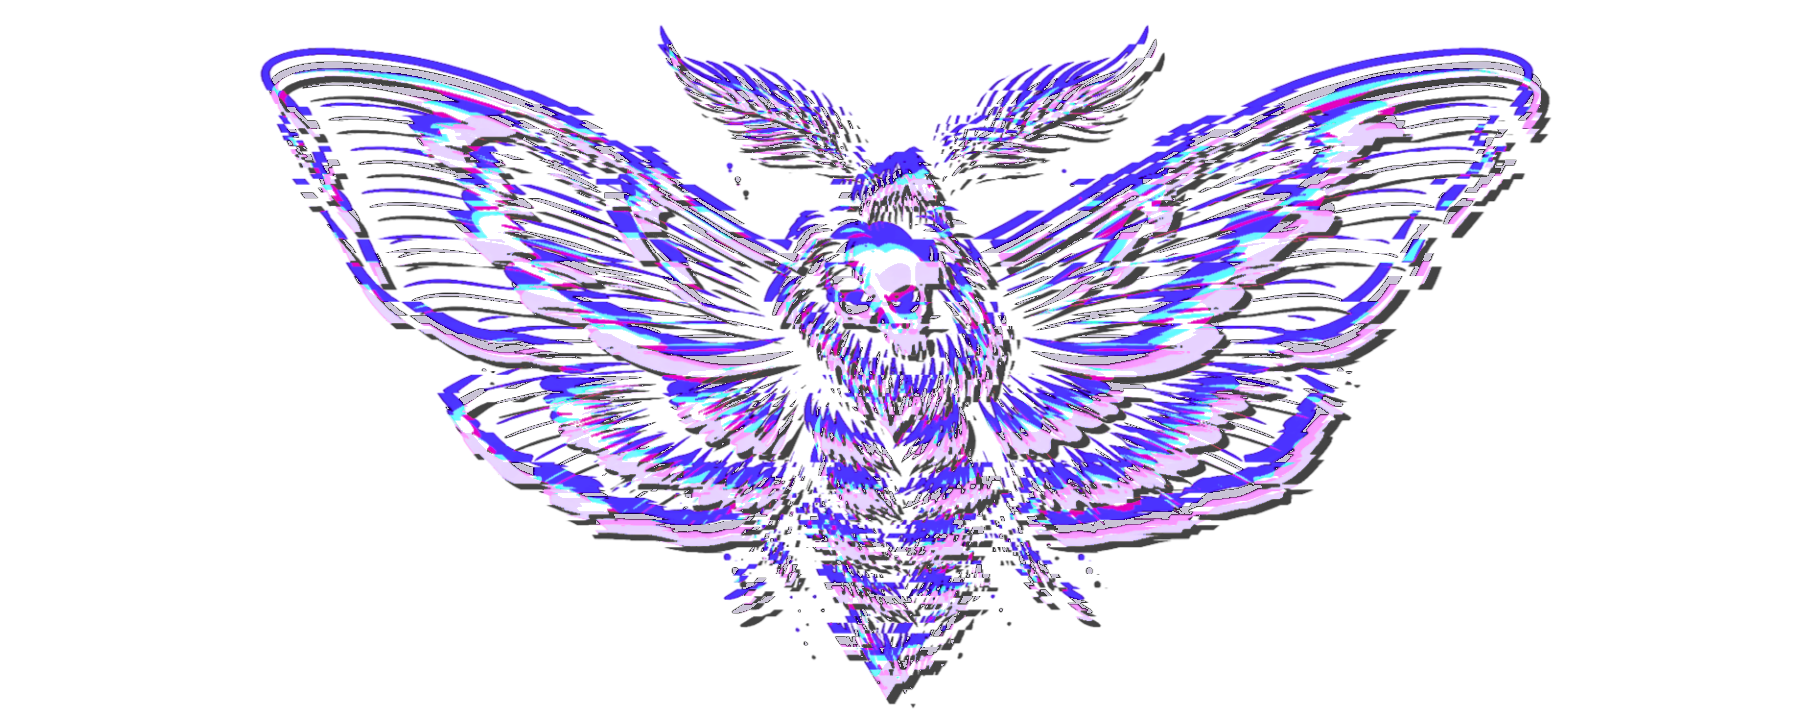
\includegraphics[width=#1]{assets/moth-cover.png}%
  }{%
    \PackageWarning{copy-fail}{assets/moth-cover.png not found; cover moth omitted}%
    \mbox{}%
  }%
}

% ============================================================
% COVER ART
% All coordinates below use millimetres inside a 210 x 297 mm panel.
% ============================================================

\tikzset{
  cover-small/.style={
    font=\displayfont\fontsize{7.2}{8.5}\selectfont,
    text=MoriGray
  },
  cover-key/.style={
    font=\displayfont\bfseries\fontsize{6.8}{8}\selectfont,
    text=MoriGray
  },
  cover-value/.style={
    font=\displayfont\bfseries\fontsize{8.2}{9.5}\selectfont,
    text=MoriPaper
  }
}

\newcommand{\DrawFrontPanel}{%
  \fill[MoriNight] (-3,-3) rectangle (213,300);

  % Fine dossier rule and outer-edge accent.
  \draw[MoriPurple,line width=0.65pt] (18,276) -- (192,276);
  \fill[MoriPurple] (205,0) rectangle (210,297);

  % Front cover: place the moth body at the binding edge (left), allowing
  % the wing to open outward across the front instead of being cut at trim.
  \node[anchor=north west,inner sep=0pt,opacity=0.50]
    at (-250,197) {\MothGraphic{500mm}};

  % Ghosted CVE number.
  \node[
    anchor=south east,
    inner sep=0pt,
    text=MoriPanel,
    font=\displayfont\bfseries\fontsize{42}{42}\selectfont
  ] at (192,5) {31431};

  % Header.
  \node[
    anchor=west,
    font=\displayfont\bfseries\fontsize{7.8}{9}\selectfont,
    text=MoriLavender
  ] at (18,263) {TECHNICAL SECURITY RESEARCH REPORT};
  \node[
    anchor=east,
    font=\ttfamily\bfseries\fontsize{8.4}{9}\selectfont,
    text=MoriPurple
  ] at (192,263) {CVE-2026-31431};

  % Main title.
  \node[
    anchor=west,
    inner sep=0pt,
    font=\displayfont\bfseries\fontsize{42}{44}\selectfont,
    text=MoriPaper
  ] at (18,221) {COPY \textcolor{MoriPurple}{FAIL}};

  \node[
    anchor=north west,
    inner sep=0pt,
    text width=154mm,
    align=left,
    font=\displayfont\fontsize{18}{21}\selectfont,
    text=MoriPaper
  ] at (18,207) {A Controlled Reproduction, Detection,\\
    and Mitigation of a Linux Kernel\\
    Local Privilege Escalation};

  \node[
    anchor=west,
    inner sep=0pt,
    font=\displayfont\bfseries\fontsize{7.1}{8}\selectfont,
    text=MoriGray
  ] at (18,151) {LINUX KERNEL\enspace
    \textcolor{MoriPurple}{\textbullet}\enspace
    LOCAL PRIVILEGE ESCALATION\enspace
    \textcolor{MoriPurple}{\textbullet}\enspace
    CONTROLLED LAB};

  % Front-cover evidence panel.
  \fill[MoriPanel,opacity=0.94] (18,25) rectangle (192,65);
  \draw[MoriMuted,line width=0.35pt] (18,25) rectangle (192,65);
  \fill[MoriPurple] (18,25) rectangle (19,65);

  \node[cover-key,anchor=north west] at (24,59) {AUTHOR};
  \node[cover-value,anchor=north west] at (24,53) {Denis Krüger};
  \node[cover-key,anchor=north west] at (83,59) {PROJECT};
  \node[cover-value,anchor=north west] at (83,53) {Copy Fail Security Lab};
  \node[cover-key,anchor=north west] at (146,59) {SEVERITY};
  \node[cover-value,anchor=north west] at (146,53) {High / CVSS 7.8};

  \node[cover-key,anchor=north west] at (24,43) {ENVIRONMENT};
  \node[cover-value,anchor=north west] at (24,37) {Isolated Proxmox Lab};
  \node[cover-key,anchor=north west] at (83,43) {FOCUS};
  \node[cover-value,anchor=north west] at (83,37) {Reproduce / Detect / Mitigate};
  \node[cover-key,anchor=north west] at (146,43) {REPORT DATE};
  \node[cover-value,anchor=north west] at (146,37) {\ReportDate};

  \node[cover-small,anchor=west] at (18,13)
    {Security research laboratory project};
  \node[cover-small,anchor=east] at (192,13)
    {controlled environment / documented evidence};
}

\newcommand{\DrawBackPanel}{%
  \fill[MoriNight] (-3,-3) rectangle (213,300);

  % Mirrored fore-edge accent and dossier rule.
  \fill[MoriPurple] (0,0) rectangle (5,297);
  \draw[MoriPurple,line width=0.65pt] (18,276) -- (192,276);

  % Back cover: mirror the artwork and place its body at the binding edge
  % (right), allowing the wing to open outward across the back.
  \node[anchor=north east,inner sep=0pt,opacity=0.50]
    at (460,197) {\reflectbox{\MothGraphic{500mm}}};

  % Small archive header.
  \node[
    anchor=west,
    font=\displayfont\bfseries\fontsize{7.8}{9}\selectfont,
    text=MoriLavender
  ] at (18,263) {CONTROLLED SECURITY RESEARCH};
  \node[
    anchor=east,
    font=\ttfamily\bfseries\fontsize{8.2}{9}\selectfont,
    text=MoriPurple
  ] at (192,263) {REPORT FROZEN // \ReportDateISO};

  % A single evidence-panel monologue, styled to match the metadata panel on
  % the front while leaving the lower moth wing visible around it.
  \fill[MoriPanel,opacity=0.90] (18,103) rectangle (192,247);
  \draw[MoriMuted,line width=0.35pt] (18,103) rectangle (192,247);
  \fill[MoriPurple] (18,103) rectangle (19,247);

  \node[
    anchor=north west,
    inner sep=0pt,
    font=\displayfont\bfseries\fontsize{13.4}{15}\selectfont,
    text=MoriPurple
  ] at (25,235) {SO, WHY DID I DECIDE TO DO THIS?};

  \node[
    anchor=north west,
    inner sep=0pt,
    text=MoriPaper
  ] at (25,218) {%
    \begin{minipage}{154mm}
      \displayfont\fontsize{10.7}{13.8}\selectfont
      \setlength{\parskip}{0.58em}
      \raggedright
      {\bfseries Honestly? Curiosity.}

      Reading ``Linux kernel local privilege escalation'' and thinking
      ``huh, interesting'' was apparently not where my brain intended to stop.

      I wanted to know whether I could reproduce \emph{Copy Fail} safely. Once
      I could, I wanted to understand what the system exposed while it happened.
      Then detect it. Then contain it. Then verify the vendor fix.

      Each answer produced another question, another test, and---somehow---another
      section.

      I did not start this project knowing exactly how every part would work. I
      started with an isolated Proxmox lab and the slightly unreasonable belief
      that, if I documented everything carefully enough, I could figure it out.

      Somewhere along the way, that became an eBPF monitor, a compensating
      control, a vendor-mitigation retest, and 146 pages of evidence.

      {\bfseries This report is what happened next.}
    \end{minipage}%
  };

  \draw[MoriMuted,line width=0.3pt] (25,124) -- (185,124);
  \node[
    anchor=west,
    inner sep=0pt,
    font=\displayfont\bfseries\fontsize{6.7}{8}\selectfont,
    text=MoriPurple
  ] at (25,114) {CURIOSITY // EVIDENCE // REPRODUCIBILITY};
  \node[
    anchor=east,
    inner sep=0pt,
    font=\ttfamily\bfseries\fontsize{6.7}{8}\selectfont,
    text=MoriLavender
  ] at (185,114) {REPORT FROZEN // \ReportDateISO};

  \draw[MoriPurple,line width=0.65pt] (18,18) -- (192,18);
  \node[cover-small,anchor=west] at (18,10)
    {DENIS KRÜGER // 0N1S3C};
  \node[cover-small,anchor=east] at (192,10)
    {146 PAGES // CVE-2026-31431};
}

% ------------------------------------------------------------
% A4 front and back pages used in normal report mode
% ------------------------------------------------------------

\newcommand{\MakeFrontCover}{%
  \begin{titlepage}
    \thispagestyle{empty}
    \begin{tikzpicture}[remember picture,overlay,x=1mm,y=1mm]
      \begin{scope}[shift={(current page.south west)}]
        \clip (0,0) rectangle (210,297);
        \DrawFrontPanel
      \end{scope}
    \end{tikzpicture}
    \null
  \end{titlepage}%
}

\newcommand{\MakeBackCover}{%
  \clearpage
  \thispagestyle{empty}
  \begin{tikzpicture}[remember picture,overlay,x=1mm,y=1mm]
    \begin{scope}[shift={(current page.south west)}]
      \clip (0,0) rectangle (210,297);
      \DrawBackPanel
    \end{scope}
  \end{tikzpicture}
  \null
  \clearpage
}

% ------------------------------------------------------------
% One-piece print wrap used in print-wrap mode
% ------------------------------------------------------------

\newcommand{\MakePrintWrap}{%
  \thispagestyle{empty}
  \begin{tikzpicture}[remember picture,overlay]
    % Continuous full-bleed field.
    \fill[MoriNight]
      (current page.south west) rectangle (current page.north east);

    % Back panel: includes top, bottom, and outer bleed but stops at spine.
    \begin{scope}[
      shift={([xshift=\CoverBleed,yshift=\CoverBleed]current page.south west)},
      x=1mm,
      y=1mm
    ]
      \clip (-3,-3) rectangle (210,300);
      \DrawBackPanel
    \end{scope}

    % Front panel: includes top, bottom, and outer bleed but stops at spine.
    \begin{scope}[
      shift={([xshift=\dimexpr\CoverBleed+\TrimWidth+\SpineWidth\relax,
               yshift=\CoverBleed]current page.south west)},
      x=1mm,
      y=1mm
    ]
      \clip (0,-3) rectangle (213,300);
      \DrawFrontPanel
    \end{scope}

    % Spine bounds derived from the trim and bleed values.
    \coordinate (SpineSW) at
      ([xshift=\dimexpr\CoverBleed+\TrimWidth\relax]current page.south west);
    \coordinate (SpineNE) at
      ([xshift=-\dimexpr\CoverBleed+\TrimWidth\relax]current page.north east);

    \shade[left color=MoriDeepPurple,right color=MoriElectric]
      (SpineSW) rectangle (SpineNE);
    \draw[MoriNight,line width=0.8pt]
      (SpineSW) -- ($(SpineSW)+(0,\WrapHeight)$);
    \draw[MoriNight,line width=0.8pt]
      (SpineNE) -- ($(SpineNE)+(0,-\WrapHeight)$);

    \node[
      rotate=-90,
      font=\displayfont\bfseries\fontsize{15}{16}\selectfont,
      text=MoriPaper
    ] at ($(SpineSW)!0.82!(SpineNE)$) {COPY \textcolor{MoriNight}{FAIL}};

    \node[
      rotate=-90,
      font=\displayfont\fontsize{9}{10}\selectfont,
      text=MoriPaper
    ] at ($(SpineSW)!0.50!(SpineNE)$) {CVE-2026-31431};

    \node[
      rotate=-90,
      font=\displayfont\bfseries\fontsize{9}{10}\selectfont,
      text=MoriPaper
    ] at ($(SpineSW)!0.18!(SpineNE)$) {DENIS KRÜGER};
  \end{tikzpicture}
  \null
  \clearpage
}

% ============================================================
% DOCUMENT
% ============================================================

\begin{document}

\ifPrintWrap

  % Print-wrap mode intentionally produces exactly one oversized page.
  \hypersetup{pageanchor=false}
  \pagestyle{empty}
  \MakePrintWrap

\else

  % ----------------------------------------------------------
  % Front cover
  % ----------------------------------------------------------

  \hypersetup{pageanchor=false}
  \MakeFrontCover
  \color{MoriInk}
  \hypersetup{pageanchor=true}

  % ----------------------------------------------------------
  % Front matter
  % ----------------------------------------------------------

  \pagenumbering{roman}

  \section*{Abstract}
  \addcontentsline{toc}{section}{Abstract}

  \begin{tcolorbox}[
    enhanced,
    breakable,
    sharp corners,
    frame hidden,
    colback=MoriPaper,
    borderline west={2.4pt}{0pt}{MoriPurple},
    left=4mm,
    right=2mm,
    top=1mm,
    bottom=1mm
  ]
  This report documents the controlled analysis, reproduction, detection,
  mitigation, and retesting of CVE-2026-31431, commonly referred to as
  \emph{Copy Fail}.

  The research is conducted within an isolated laboratory environment and
  focuses not only on demonstrating the vulnerability, but on understanding
  the affected Linux kernel functionality, identifying observable behaviour,
  developing a custom detection strategy, evaluating a compensating control,
  and comparing those results with vendor-provided mitigations and patches.

  Evidence is collected throughout the experiment and preserved separately
  from the analytical report. Raw evidence is retained privately, while
  sanitized artifacts intended for public release receive their own integrity
  verification before being added to the repository.
  \end{tcolorbox}

  \clearpage
  \markboth{Contents}{}
  \tableofcontents
  \clearpage

  % ----------------------------------------------------------
  % Main report
  % ----------------------------------------------------------

  \pagenumbering{arabic}

  \section{Introduction and Vulnerability Overview}

\subsection{Vulnerability Overview}

This report investigates CVE-2026-31431, commonly referred to as
\emph{Copy Fail}, a local privilege escalation vulnerability in the Linux
kernel. The goal is to reproduce the vulnerability in an isolated laboratory
environment, understand the underlying bug, and use the observed behaviour to
develop and test detection and mitigation approaches.

The vulnerability affects \code{algif\_aead}, the Linux kernel's userspace
interface for AEAD algorithms exposed through \code{AF\_ALG} sockets. The
vulnerable code incorrectly performs cryptographic operations in place even
though the source and destination originate from different mappings. Combined
with \code{splice()}, this can cause page-cache-backed data from a readable file
to become part of a writable cryptographic scatterlist. Under the right
conditions, an unprivileged process can therefore modify the cached contents
of a file without having write permission to the file itself
\cite{ubuntu-copyfail-cve,linux-copyfail-fix}.

The published Copy Fail research turns this behaviour into a deterministic,
attacker-controlled four-byte write into the page cache of a readable file.
By repeatedly applying this primitive to a suitable setuid-root executable,
an otherwise unprivileged local user can modify the cached executable image
and ultimately execute code with root privileges
\cite{copyfail-research}.

Canonical classifies CVE-2026-31431 as a High-severity vulnerability with a
CVSS 3.1 score of 7.8. Besides local privilege escalation on the host,
Canonical also notes that the vulnerability may facilitate container escape
scenarios in affected environments
\cite{ubuntu-copyfail-cve}.

For this project, however, the interesting part is not simply whether the
published exploit can produce a root shell. The more useful question is what
actually happens on the system while the vulnerability is being exploited,
which parts of that behaviour can be observed, and whether the exploitation
path can be detected or restricted before the vendor patch is applied.

\subsection{Technical Background and Vulnerability Mechanism}

To understand Copy Fail, it is important to distinguish between a file on disk
and the copy of its contents currently held in memory. Linux uses the page
cache to keep recently accessed file data in memory, allowing subsequent reads
and executions to use the cached pages instead of repeatedly accessing the
underlying storage. A process with read access to a file may therefore cause
its contents to enter the page cache, but this should not give that process the
ability to modify those contents.

Copy Fail breaks this assumption through an unexpected interaction between the
page cache and the Linux kernel crypto API. Linux exposes parts of this API to
userspace through \code{AF\_ALG} sockets. For authenticated encryption,
\code{algif\_aead} provides the corresponding AEAD interface. AEAD
(Authenticated Encryption with Associated Data) combines encryption with
integrity protection and allows additional authenticated data to be included
without encrypting it.

Internally, cryptographic operations use scatterlists to describe the different
regions of memory involved in an operation. In the vulnerable implementation,
\code{algif\_aead} performs AEAD operations in place, meaning that the source
and destination of the cryptographic request ultimately share the same
scatterlist. This becomes problematic because the input and output do not
necessarily originate from the same type of memory
\cite{copyfail-research,linux-copyfail-fix}.

The second important part of the vulnerability is \code{splice()}. This system
call can move data between file descriptors without first copying it through a
conventional userspace buffer. When data from a readable file is spliced through
a pipe into an \code{AF\_ALG} socket, references to the file's page-cache pages
can become part of the crypto input scatterlist. During AEAD decryption,
\code{algif\_aead} copies the associated data and ciphertext into the receive
buffer, but chains the authentication-tag region from the original input onto
the destination scatterlist. As a result, file-backed page-cache memory can
become reachable through a scatterlist that the cryptographic operation treats
as writable \cite{copyfail-research}.

This alone does not yet produce the controlled write used by Copy Fail. The
final piece is the \code{authencesn} AEAD template. During decryption,
\code{authencesn} temporarily rearranges IPsec Extended Sequence Number data
and uses the destination scatterlist as scratch space. As part of this process,
it performs a four-byte write beyond the legitimate AEAD output region. Under
normal circumstances this affects the operation's destination buffer. Combined
with the vulnerable in-place layout in \code{algif\_aead}, however, that write
can instead reach one of the chained page-cache pages
\cite{copyfail-research}.

The attacker can control both the position of this write and the four-byte
value being written. Even though the subsequent authentication check fails,
the modification is not rolled back. The affected page is also not marked
dirty for normal filesystem writeback, meaning the file on disk remains
unchanged while its cached in-memory representation has been modified. The
result is therefore a deterministic four-byte write into the page cache of a
file that the attacker only needs permission to read
\cite{copyfail-research}.

This limited primitive is the central building block of Copy Fail. It does not
grant root privileges by itself, but it creates something much more interesting
from an exploitation perspective: the ability to modify executable data in
memory without having normal write access to the underlying file. How this
primitive is turned into privilege escalation is discussed in the following
section.

\subsection{Security Impact}

At first glance, a controlled four-byte write may appear too limited to be useful
for privilege escalation. The important limitation, however, is only the amount
of data written during a single operation. Because the primitive is deterministic
and repeatable, an attacker can perform multiple writes at controlled offsets and
gradually modify a larger region of a cached file
\cite{copyfail-research}.

The published Copy Fail exploit demonstrates this by targeting
\code{/usr/bin/su}, a setuid-root executable commonly available on Linux systems.
Successive four-byte writes are used to modify executable code in the cached
image of the binary. The file itself remains owned by root and retains its setuid
permissions because neither its filesystem metadata nor its persistent contents
need to be changed.

When the modified executable is started, Linux uses the poisoned page-cache
contents while still applying the privileges associated with the original
setuid-root file. The injected code therefore executes in a privileged context,
allowing a local unprivileged user to obtain root privileges. In other words, the
attacker never needs legitimate write access to the executable. Read access,
combined with the vulnerable kernel path, is enough to cross the privilege
boundary \cite{copyfail-research}.

An additional characteristic of Copy Fail is that the corrupted page is not
marked dirty for normal filesystem writeback. The modification therefore exists
in memory while the corresponding data on persistent storage remains unchanged.
This makes the corruption temporary from the filesystem's perspective, but that
does not reduce its immediate impact: the attacker only needs the modified
executable to run once to turn the page-cache write into a root shell
\cite{copyfail-research}.

The impact is also not necessarily limited to processes running directly on the
host. Canonical notes that the same vulnerability may facilitate container escape
scenarios in affected environments, extending the security implications beyond
a conventional local privilege escalation
\cite{ubuntu-copyfail-cve}.

The significance of Copy Fail is therefore much larger than the size of the
individual write suggests. A four-byte primitive is enough to undermine the
integrity of privileged executable code and ultimately turn an unprivileged local
user into root.

\subsection{Vendor Response and Mitigation}

Following the public disclosure of Copy Fail, Canonical initially provided a
temporary mitigation that removed access to the vulnerable kernel path rather
than attempting to correct the underlying bug. An update to the \code{kmod}
package prevented the \code{algif\_aead} module from being loaded, making the
affected AF\_ALG AEAD interface unavailable through that module
\cite{ubuntu-copyfail-cve}.

If the module was already loaded, it additionally had to be unloaded or the
system rebooted for the mitigation to become effective. Canonical explicitly
treated this as a temporary measure. Applications that rely on the kernel AEAD
interface may fall back to userspace cryptographic implementations, but this
behaviour is not guaranteed and disabling the module may therefore cause
compatibility or functionality problems
\cite{ubuntu-copyfail-cve}.

The original Copy Fail research also proposes restricting the attack surface by
preventing creation of AF\_ALG sockets through mechanisms such as seccomp. Like
disabling \code{algif\_aead}, this can prevent the vulnerable path from being
reached, but it does not correct the vulnerability itself
\cite{copyfail-research}.

The central upstream fix instead addresses the underlying design problem in
\code{algif\_aead}. The kernel change titled
\emph{Revert to operating out-of-place} removes the problematic in-place
operation introduced by an earlier optimization. Because the source and
destination originate from different mappings, the kernel developers concluded
that there was no practical benefit in sharing the same buffers. Restoring
out-of-place operation keeps the cryptographic destination separate from the
file-backed input pages and removes the condition that allowed page-cache memory
to become writable through the AEAD operation
\cite{linux-copyfail-fix}.

Distribution kernel updates include this change together with related fixes in
the AF\_ALG and authentication code. Once a corrected kernel is installed and
the system has been rebooted into it, the temporary module-level mitigation is
no longer required. Canonical therefore recommends updating to a fixed kernel
instead of relying permanently on disabling \code{algif\_aead}
\cite{ubuntu-copyfail-cve}.

This distinction is important for the experimental part of this project.
Disabling the vulnerable interface can stop exploitation, but it does so by
removing functionality. The kernel patch instead removes the vulnerable
behaviour itself. Both approaches provide useful reference points when evaluating
whether additional detection or mitigation techniques can identify or interrupt
Copy Fail without simply disabling the affected subsystem.

\subsection{Research Objectives and Questions}

The objective of this project is not limited to successfully executing the
published Copy Fail proof of concept. Reproducing the privilege escalation is
treated as the starting point for a broader investigation into how the
vulnerability behaves, how that behaviour can be observed, and which defensive
measures can meaningfully interrupt the exploitation path.

The experimental workflow therefore follows the vulnerability through several
states: first understanding and reproducing it, then observing and detecting its
behaviour, applying a compensating control, comparing that control with the
vendor mitigation, and finally retesting against a patched kernel.

The investigation is guided by the following research questions:

\begin{description}

    \item[RQ1 Reproduction.]
    Can Copy Fail be reproduced reliably in the isolated laboratory environment
    by an ordinary, unprivileged local user?

    \item[RQ2 Observability.]
    Which system-level behaviours can be observed consistently while the
    vulnerability is being exploited, and which of these provide useful
    detection opportunities?

    \item[RQ3 Detection.]
    Can the exploitation technique be detected using behavioural indicators
    rather than artifacts that are specific to a particular proof of concept,
    such as its filename or executable hash?

    \item[RQ4 Compensating Control.]
    Can a defensive control interrupt the known exploitation path before the
    kernel is patched, and can it do so without unnecessarily removing benign
    functionality?

    \item[RQ5 Vendor Comparison.]
    How does the custom compensating control compare with Canonical's temporary
    mitigation, which prevents \code{algif\_aead} from being loaded?

    \item[RQ6 Patch Validation.]
    Does reproduction fail after installation of a corrected kernel, and do the
    observations from the final retest match the expected behaviour of the
    upstream fix?

\end{description}

Together, these questions turn the published exploit into an experimental
starting point rather than the final result. A successful root shell proves that
the vulnerability can be reproduced, but the more useful outcome is understanding
what distinguishes the vulnerable behaviour, how defenders can react to it, and
what changes once the underlying kernel flaw is actually removed.

\subsection{Scope and Safety}

All experimentation in this project is restricted to systems owned and
controlled for the purpose of the research and placed inside an isolated
laboratory environment. No third-party or internet-facing systems are included
in the test scope. The deliberately vulnerable reproduction target is kept
separate from the patched reference system so that a known-good comparison state
remains available throughout the project.

Reproduction is performed from a dedicated unprivileged local account. For the
purpose of this project, privilege escalation is considered successfully
demonstrated once that account can execute a process with UID 0 and the result
can be recorded using a minimal command such as \code{id}. No persistence,
credential theft, lateral movement, or unrelated post-exploitation activity is
required or performed.

The experimental scope is limited to the published Copy Fail exploitation path
involving the AF\_ALG AEAD interface and modification of file-backed page-cache
contents. Potential container escape is relevant to the vulnerability's overall
impact, but it is not reproduced as part of this project. Other Linux kernel
vulnerabilities and unrelated privilege-escalation techniques are likewise
outside the scope of the experiment.

System state is recorded before vulnerability-specific changes or exploit
execution. Snapshots and phase checkpoints are used so that an ambiguous or
modified system can be restored rather than treated as a clean reference.
Experimental evidence is collected separately from the analytical report. Raw
artifacts are preserved privately with integrity verification, while material
intended for public release is sanitized where necessary and receives separate
integrity verification after sanitization.

These boundaries keep the experiment focused on understanding, observing, and
defending against Copy Fail while ensuring that the reproduction remains
controlled, reversible, and limited to the behaviour required to answer the
research questions.
  \clearpage
  \section{Laboratory Setup and Methodology}
\label{sec:lab-setup}

% Support compilation either from report/ or from the repository root.
\graphicspath{{../evidence/}{evidence/}}

\subsection{Laboratory Purpose and Scope}

The laboratory was designed to support controlled comparison across the
different stages of the Copy Fail investigation. Its purpose was not merely to
provide a system on which the published proof of concept could be executed.
The environment also needed to preserve a trustworthy reference state, allow a
historically vulnerable state to be reconstructed deliberately, and support
later detection, mitigation, and patch-validation experiments under comparable
conditions.

The design followed four rules. First, all vulnerability-specific activity was
confined to an isolated, privately owned virtual network. Second, the patched
reference system and the vulnerable reproduction target were maintained as
separate virtual machines rather than as successive states of one machine.
Third, reproduction began from a dedicated local account without administrative
privileges, so a later UID~0 result could be compared with a documented
unprivileged starting state. Finally, each experimental phase was treated as a
separate checkpoint and preserved with the applicable combination of command
output, screenshots, configuration artifacts, and integrity manifests.

This design separates the system state used for comparison from the state
being modified during experimentation. It also allows observations from later
phases to be interpreted against documented preconditions instead of relying
on an increasingly mutated virtual machine. The following sections describe
the infrastructure, network isolation, virtual-machine roles, account
separation, experimental sequence, and evidence-handling process used to
maintain that distinction.

\subsection{Infrastructure and Network Isolation}

The laboratory was hosted on a Dell OptiPlex 5070 Micro running Proxmox
VE~9.2.5. The host provided an Intel Core i5-9500T processor and approximately
31~GiB of memory. These specifications establish the scale of the environment,
but the experiment did not depend on specialised hardware. Both Copy Fail test
systems were conventional x86-64 KVM/QEMU virtual machines.

\begin{table}[H]
    \centering
    \caption{Relevant laboratory infrastructure and network roles.}
    \label{tab:lab-infrastructure}
    \small
    \begin{tabularx}{\textwidth}{@{}>{\bfseries}p{0.27\textwidth}Y@{}}
        \toprule
        Component & Configuration and role \\
        \midrule
        Physical host &
        Dell OptiPlex 5070 Micro, Intel Core i5-9500T, approximately 31~GiB RAM \\

        Hypervisor &
        Proxmox VE~9.2.5 using KVM/QEMU virtualization \\

        Laboratory gateway &
        OPNsense virtual firewall separating the management-facing and internal
        laboratory segments \\

        Management bridge &
        \code{vmbr0}, connected to the ordinary management network and to the
        management-facing interface of OPNsense \\

        Internal bridge &
        \code{vmbr1}, providing the isolated Layer-2 segment used by the Copy
        Fail guest systems \\

        Guest attachment &
        A single virtual network interface on \code{vmbr1}; addressing and the
        default gateway were provided within the laboratory subnet \\
        \bottomrule
    \end{tabularx}
\end{table}

The logical network path is shown in \cref{fig:lab-topology}. Private IP
addresses, MAC addresses, and unrelated details of the surrounding home
network are intentionally omitted because they do not affect reproduction of
the experiment.

\begin{figure}[H]
    \centering
    \begin{tikzpicture}[
        infrastructure/.style={
            draw=MoriRule,
            fill=MoriCode,
            text=MoriInk,
            minimum width=6.2cm,
            minimum height=0.9cm,
            align=center,
            font=\displayfont\small
        },
        boundary/.style={
            draw=MoriPurple,
            fill=MoriMist,
            text=MoriInk,
            line width=0.8pt,
            minimum width=6.2cm,
            minimum height=0.95cm,
            align=center,
            font=\displayfont\small\bfseries
        },
        guest/.style={
            draw=MoriRule,
            fill=MoriPaper,
            text=MoriInk,
            minimum width=5.4cm,
            minimum height=1.05cm,
            align=center,
            font=\displayfont\small
        },
        path/.style={
            <->,
            line width=0.75pt,
            draw=MoriMuted
        },
        pathlabel/.style={
            fill=MoriPaper,
            inner sep=2pt,
            text=MoriDeepPurple,
            font=\ttfamily\scriptsize
        }
    ]
        \node[infrastructure] (management) at (0,0)
            {Home / management network};
        \node[boundary] (firewall) at (0,-1.8)
            {OPNsense firewall and laboratory gateway};
        \node[infrastructure] (laboratory) at (0,-3.6)
            {Isolated laboratory LAN};
        \node[guest] (reference) at (-3.15,-5.35)
            {VM 270\\Patched reference system};
        \node[guest] (vulnerable) at (3.15,-5.35)
            {VM 271\\Vulnerable reproduction target};

        \draw[path] (management) -- node[pathlabel] {vmbr0} (firewall);
        \draw[path] (firewall) -- node[pathlabel] {vmbr1} (laboratory);
        \draw[->,line width=0.75pt,draw=MoriMuted]
            (laboratory.south) -- ++(0,-0.45) -| (reference.north);
        \draw[->,line width=0.75pt,draw=MoriMuted]
            (laboratory.south) -- ++(0,-0.45) -| (vulnerable.north);
    \end{tikzpicture}
    \caption{Logical separation between the management network and the Copy
    Fail guest systems.}
    \label{fig:lab-topology}
\end{figure}

Neither Copy Fail guest was attached directly to \code{vmbr0}. Their only
virtual network interface was connected to \code{vmbr1}, so communication
between the laboratory segment and the ordinary management network crossed the
OPNsense policy boundary. This prevented the deliberately vulnerable systems
from sharing the ordinary network's Layer-2 segment while retaining controlled
administrative access when required. The vulnerability itself was exercised
locally inside VM~271; no third-party or internet-facing target formed part of
the test path.

\subsection{Virtual-Machine Roles and State Separation}

The two Copy Fail guests shared a controlled starting configuration. VM~270,
\code{copyfail01}, ran Ubuntu Server 24.04.2 LTS with two virtual CPUs, 4~GiB of
memory, a 32~GiB virtual disk, and one \code{vmbr1} network interface. Once it
had been established as a patched reference, VM~271, \code{copyfail-vuln}, was
created as a full clone. The clone retained the same operating-system lineage
and virtual-hardware profile, but its machine identity and SSH host keys were
regenerated so that the guests no longer shared host identity.

The guest baseline for VM~270 is preserved under
\path{evidence/00-baseline/}. The sanitized hypervisor supplement
\path{evidence-audit/vm270-proxmox-state-public.txt} records its virtual CPU,
memory, disk, \code{vmbr1} attachment, and snapshot ancestry without publishing
the original machine identifiers. The public package does not contain an
equivalent Proxmox configuration transcript for VM~271, so the clone procedure
is reported as laboratory methodology while later phase captures establish the
runtime state actually used for each experiment.

The virtual machines were assigned different roles before reconstruction.
VM~270 was preserved as the known-good comparison system and was not downgraded
or repeatedly reconfigured for exploit testing. VM~271 was the only guest
deliberately modified for vulnerable-kernel reconstruction, reproduction,
detection, mitigation, and validation. \Cref{tab:vm-roles} summarizes this
division.

\begin{table}[H]
    \centering
    \caption{Virtual-machine roles and permitted state changes.}
    \label{tab:vm-roles}
    \small
    \begin{tabularx}{\textwidth}{@{}>{\bfseries\raggedright\arraybackslash}p{0.20\textwidth}p{0.25\textwidth}Y@{}}
        \toprule
        Virtual machine & Experimental role & Permitted state changes \\
        \midrule
        VM 270 \code{copyfail01} &
        Patched reference &
        Preserved as the known-good comparison state; no deliberate
        vulnerable reconstruction \\

        VM 271 \code{copyfail-vuln} &
        Experimental target &
        Vulnerable reconstruction, reproduction, detection, mitigation, and
        validation activities \\
        \bottomrule
    \end{tabularx}
\end{table}

Although the guests were not independent experimental samples, cloning reduced
irrelevant starting differences and state separation protected the reference
from destructive work. Comparisons therefore used a preserved control rather
than an undocumented earlier state of the modified target.

\subsection{Account and Privilege Separation}

Privileged laboratory preparation and unprivileged test execution were assigned
to separate local accounts. The \code{researcher} account, with UID~1000 and
primary GID~1000, provided the administrative context required for kernel
management, package and service configuration, instrumentation, and evidence
collection. Its recorded memberships included the administrative groups
\code{adm}, \code{sudo}, and \code{lxd}. Root authority was used where these
tasks required it, but neither the administrative account nor an existing root
shell formed part of the attacker execution context.

The dedicated \code{labuser} account, with UID~1001 and primary GID~1001,
represented an attacker-controlled but initially unprivileged local foothold.
Its recorded supplementary membership was limited to the ordinary
\code{users} group (GID~100); it was not assigned membership in administrative
groups such as \code{sudo} or \code{lxd}. The threat model therefore assumed
that an attacker had already obtained command execution as this ordinary
account; the preceding compromise was not reproduced. The vulnerable-kernel
reproduction and MORI enforcement trials used this account as their attacker
context. The patched-kernel phase recorded the identity again for each retest
rather than assuming it was unchanged: notably, its Python retest used the
\code{researcher} account. That run can show that no automatic UID~0 transition
was observed in its recorded context, but it is not an identity-matched repeat
of the vulnerable \code{labuser} execution. \Cref{tab:account-roles} summarizes
the resulting separation of duties.

\begin{table}[H]
    \centering
    \caption{Account roles and privilege contexts used in the laboratory.}
    \label{tab:account-roles}
    \small
    \begin{tabularx}{\textwidth}{@{}>{\bfseries\raggedright\arraybackslash}p{0.20\textwidth}p{0.28\textwidth}Y@{}}
        \toprule
        Account & Starting context & Laboratory role \\
        \midrule
        \code{researcher} (UID 1000) &
        Administrative; member of \code{adm}, \code{sudo}, and \code{lxd} &
        Environment preparation, instrumentation, and privileged evidence
        collection \\

        \code{labuser} (UID 1001; GID 1001) &
        Unprivileged local user; supplementary membership limited to
        \code{users} (GID 100) &
        Primary attacker context for vulnerable-kernel reproduction and
        compensating-control tests \\
        \bottomrule
    \end{tabularx}
\end{table}

The \code{researcher} state is recorded under
\path{evidence/00-baseline/} in \path{command-output/id.txt}. The
\code{labuser} state is recorded under \path{evidence/02-reproduction/} in
\path{artifacts/01-pre-exploit-state.txt}. Later retests preserve their own
identity captures where the execution context differs.

\begin{figure}[H]
    \centering
    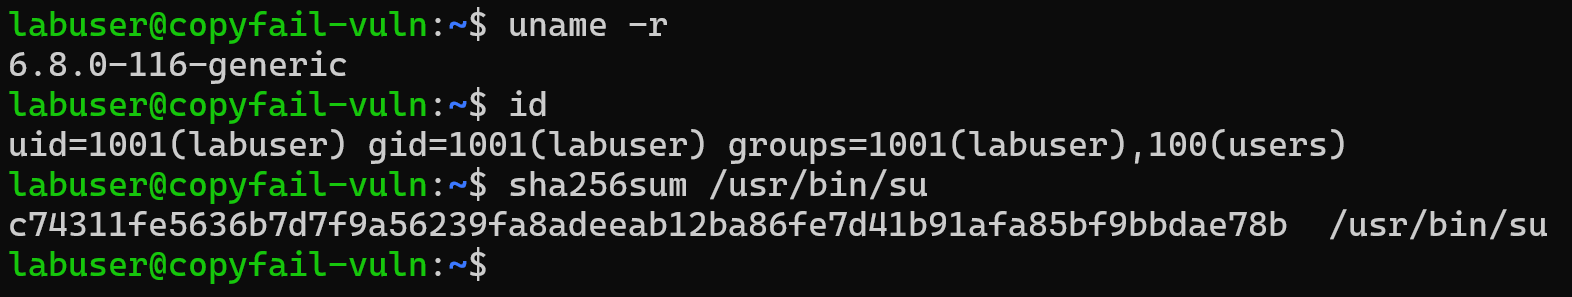
\includegraphics[
        width=\textwidth,
        height=0.36\textheight,
        keepaspectratio
    ]{02-reproduction/screenshots/01-pre-exploit-state.png}
    \caption{Recorded vulnerable-kernel starting state: kernel
    \code{6.8.0-116-generic}, \code{labuser} as UID~1001, its non-administrative
    group membership, and the baseline digest of \code{/usr/bin/su}.}
    \label{fig:labuser-pre-exploit-state}
\end{figure}

The screenshot in \cref{fig:labuser-pre-exploit-state} is the visual capture
paired with the machine-readable pre-exploit artifact. Together they establish
the starting privilege boundary used for the vulnerable-kernel reproduction.

Before each relevant trial, the active identity and privilege state were
recorded from the test account. Keeping preparation and execution contexts
separate prevents an inherited administrative session, a \code{sudo}-launched
process, or a pre-existing root shell from being mistaken for successful local
privilege escalation. Any later change in effective privilege could therefore
be evaluated against the identity recorded for that trial rather than being
confused with laboratory setup.

\subsection{Threat Model and Security Objectives}

The threat model begins after initial access has already occurred. The attacker
is assumed to control the local \code{labuser} account and therefore starts with
command execution as UID~1001 rather than with administrative authority. From
this foothold, the attacker may execute arbitrary local programs, invoke kernel
interfaces available to an ordinary user, and interact with readable privileged
executables. The attacker may also choose the proof-of-concept implementation,
create processes or threads, arrange relevant system calls, and introduce
delays under their control. The preceding compromise of \code{labuser} is an
assumed precondition and is not itself reproduced.

At the start of an attempt, the attacker does not possess UID~0, membership in
\code{sudo} or \code{lxd}, administrative credentials, or ordinary write access
to the targeted SUID executable. The relevant trust boundary is therefore the
transition from the unprivileged UID~1001 context to root authority. Copy Fail
threatens that boundary by combining the accessible AF\_ALG AEAD and
\code{splice()} paths with modification of file-backed page-cache contents
belonging to a readable privileged executable. The protected assets are both
the integrity of privileged executable code and the authority obtained when
that code is executed with UID~0.

The experiment evaluates the objectives in \cref{tab:security-objectives}.
These criteria distinguish observation from enforcement and separate a
compensating control from correction of the underlying kernel flaw.

\begin{table}[H]
    \centering
    \caption{Security objectives derived from the experimental threat model.}
    \label{tab:security-objectives}
    \small
    \begin{tabularx}{\textwidth}{@{}>{\bfseries\raggedright\arraybackslash}p{0.22\textwidth}Y@{}}
        \toprule
        Objective & Required property \\
        \midrule
        Privilege-boundary protection &
        Prevent an unauthorised transition from the documented UID~1001
        starting context to UID~0. \\

        Executable integrity &
        Preserve the contents and security-relevant state of the targeted
        privileged executable during a prevented attempt. \\

        Behavioural detection &
        Identify the exploitation behaviour without depending on a particular
        proof-of-concept filename, programming language, or executable hash. \\

        Selective correlation &
        Associate the relevant operations within the attacker-controlled
        execution context while avoiding attribution across unrelated
        processes and remaining robust against attacker-controlled timing. \\

        Compatibility &
        Preserve the specific benign interface operations selected for control
        testing and state clearly which wider functionality was not exercised. \\

        Patch independence &
        Verify that a corrected kernel prevents the tested escalation path
        without relying on the custom compensating control. \\
        \bottomrule
    \end{tabularx}
\end{table}

Observation alone does not satisfy the prevention objective. A mechanism is
treated as preventive only if it interrupts the attempted privilege escalation
and the protected target retains its integrity. Likewise, the custom
compensating control is expected to act on the correlated exploitation path
rather than on one known proof-of-concept artifact. Compatibility is evaluated
separately so that removing the vulnerable interface and selectively
restricting its dangerous use are not treated as equivalent defensive
properties. In this report, compatibility means only the operations exercised
by the documented controls; it is not a claim about every \code{AF\_ALG} or AEAD
workload.

The model excludes the means by which \code{labuser} was initially compromised,
remote exploitation, persistence, credential collection, reverse shells,
lateral movement, container escape, unrelated privilege-escalation techniques,
and post-root activity beyond the minimal evidence needed to establish the
privilege state. These exclusions keep the analysis focused on whether control
of an ordinary local account can be escalated through Copy Fail, and whether the
evaluated defences prevent that transition under the stated conditions.

\subsection{Experimental Sequence and State Transitions}

The investigation was organised as a sequence of controlled system states
rather than as one continuous session on an increasingly modified machine.
VM~270 remained the patched reference, while VM~271 was moved deliberately
through vulnerable reconstruction, reproduction, observation, mitigation, and
final patch-validation states. This separation provided a stable comparison
system and made the state-changing work on VM~271 explicit.

Each phase followed the same control cycle. A relevant snapshot or documented
checkpoint was first established or restored. The running kernel, required
interfaces, active account, defensive-control state, and protected target were
then checked as applicable to that phase. Evidence was collected around the
phase-specific activity, with pre-test and post-test captures used where they
were available and relevant. The resulting artifacts were preserved before
another kernel, configuration, or control change was introduced.
\Cref{tab:experimental-sequence} maps this procedure to the six public evidence
sets used by the report.

\begin{table}[H]
    \centering
    \caption{Controlled experimental sequence and state transitions.}
    \label{tab:experimental-sequence}
    \small
    \begin{tabularx}{\textwidth}{@{}>{\bfseries\raggedright\arraybackslash}p{0.16\textwidth}>{\raggedright\arraybackslash}p{0.29\textwidth}Y@{}}
        \toprule
        Evidence set & Established state & Methodological purpose \\
        \midrule
        Phase 00 &
        VM~270 preserved as the patched reference &
        Record a known-good comparison state that was not subjected to
        vulnerable reconstruction or exploit development. \\

        Phase 01 &
        VM~270 checked against the Copy Fail prerequisites and vendor state &
        Record which relevant interfaces, modules, package rules, and fixed
        kernel state were present before building the vulnerable target. \\

        Phase 02 &
        VM~271 booted into the selected historical kernel with the required
        Copy Fail interfaces available and no specific enforcement active &
        Verify the vulnerable preconditions, execute from the documented
        UID~1001 context, and record the privilege and target states. \\

        Phase 03 &
        Reproducible vulnerable state with monitoring introduced separately
        from enforcement &
        Identify observable behaviour, evaluate integrity-based monitoring,
        and compare behavioural evidence with artifact-specific detection. \\

        Phase 04 &
        Vulnerable kernel with broad restriction followed by successive MORI
        observation, correlation, shadow, and enforcement candidates &
        Compare interface removal with selective control, exercise positive and
        negative regression cases, and freeze the final vulnerable-kernel
        candidate. \\

        Phase 05 &
        VM~271 updated to the corrected kernel with MORI isolated from the
        active enforcement path &
        Record the identity used for each retest, exercise the tested interface
        operations, and repeat both proof-of-concept paths independently of the
        custom control. \\
        \bottomrule
    \end{tabularx}
\end{table}

The phase numbers correspond directly to the directories under
\path{evidence/}. Phase~04 contains several internal MORI checkpoints because
control development required more than one state transition, but those
checkpoints are engineering iterations rather than independent experimental
samples.

The order of these transitions was significant. Unmitigated reproduction was
completed before preventive mechanisms were introduced, ensuring that later
denials could be compared with a demonstrated vulnerable path. Monitoring was
introduced before selective enforcement so that candidate observables and
correlation rules could be examined without initially changing the tested
operation. Broad interface restriction showed the effect on the interface
operations selected for testing, whereas the later MORI stages progressively
narrowed the controlled behaviour through observation, correlation, shadow
evaluation, and active enforcement.

Regression testing was treated as part of control development rather than as a
single final exploit run. Trials varied the proof-of-concept implementation,
process or thread context, operation ordering, attacker-controlled delay, and
privileged target where the phase required it. Negative controls were retained
to distinguish the correlated Copy Fail path from isolated or unrelated uses of
the same system interfaces. A candidate was not treated as the current MORI
implementation until these phase-specific checks had been performed against a
documented build and system state.

Vendor remediation was applied only after the vulnerable-kernel experiments
and their checkpoints had been preserved. Isolation of MORI from the active
enforcement path was a required condition of the patched-kernel retest. The
evidence for its exact timing is not perfect: a screenshot shows the isolated
state in the retest sequence, while the timestamped machine-readable capture
was collected later. The patched result is therefore interpreted from the
combined state and execution records rather than from that timestamp alone.
The affected interface was checked separately at the \code{socket()},
\code{bind()}, and \code{accept()} stages. This confirms availability of those
tested operations, not a complete encrypt/decrypt round trip.

The phases form a dependent engineering and validation sequence rather than a
set of independent statistical samples. Their evidential value therefore rests
on the documented preconditions and adjacent pre-test and post-test captures.
Observations made after a state transition were not retroactively used to
characterise an earlier phase; where a later test exposed a new condition, that
condition was added as a prospective regression case and recorded in the state
in which it was actually exercised.

\subsection{Evidence Collection, Integrity, and Publication Workflow}

Evidence was collected alongside each experimental phase and kept separate
from the analytical report. Phase directories normally combined
machine-readable artifacts, screenshots, explanatory documentation, and an
integrity manifest. This structure allowed later claims to be traced to their
preconditions, execution, and post-test records without treating the report
narrative as primary evidence.

The evidence classes in \cref{tab:evidence-classes} served complementary
purposes; no single class was considered sufficient for every claim.

\begin{table}[H]
    \centering
    \caption{Evidence classes and their methodological roles.}
    \label{tab:evidence-classes}
    \small
    \begin{tabularx}{\textwidth}{@{}>{\bfseries\raggedright\arraybackslash}p{0.21\textwidth}>{\raggedright\arraybackslash}p{0.32\textwidth}Y@{}}
        \toprule
        Evidence class & Primary function & Inherent limitation \\
        \midrule
        Command output and logs &
        Preserve searchable kernel, identity, service, event, permission, and
        target state. &
        Only the requested commands are represented; collection can fail or
        omit context. \\

        Screenshots &
        Preserve visible terminal context, ordering, concurrent telemetry, and
        interactive outcomes. &
        Captures are selective and may omit timestamps or complete output. \\

        Configuration and source &
        Record relevant detectors, mitigations, services, policies, and test
        material. &
        Source does not establish which build was loaded or exercised. \\

        Build and provenance records &
        Associate source, generated objects, binaries, compiler context,
        revisions, and digests. &
        Provenance identifies a candidate but does not prove its runtime
        behaviour. \\

        Snapshots and checkpoints &
        Preserve recoverable system states and historical MORI implementations. &
        A checkpoint establishes recoverability, not an experimental claim
        without adjacent captures. \\
        \bottomrule
    \end{tabularx}
\end{table}

For state-changing trials, evidence was collected around the test rather than
only afterwards. Applicable pre-test captures identified the kernel, account,
interface or module state, defensive-control state, and privileged target.
Execution output and telemetry were followed by the resulting privilege and
target state. Where chronology was material, timestamps were included inside
the capture when practicable; file-system and archive modification times were
supporting metadata rather than the sole proof of event order.

Evidence numbering and phase maps preserved the recorded sequence. Missing or
removed items were not hidden by renumbering later objects. A supplemental
capture could clarify a retained state or artifact, but could not retroactively
establish an uncaptured precondition. It therefore required explicit labelling
rather than being presented as part of the original sequence. Filenames were
treated as navigation aids, not as proof of system state. If a filename and its
captured contents disagreed, the commands and output inside the capture governed
the interpretation.

Implementation provenance remained separate from runtime results. MORI
checkpoints preserved successive source, generated BPF objects, skeletons, and
userspace builds, while the validated candidate was placed under the distinct
\code{current/} path. Digests and provenance records associated the frozen
source and build artifacts with the candidate used for final regression.
Proof-of-concept provenance used available repository revisions, source and
binary hashes, compiler information, and execution captures without requiring
redistribution of the exploit implementation.

Integrity protection followed a two-stage workflow. Raw evidence was hashed
before the private original was preserved. Publication work then occurred on a
separate copy. After redaction, omission, renaming, or other sanitization, the
public package received its own SHA-256 manifest and was verified again after
assembly or transfer. Private and public digests were not interchangeable
because legitimate publication transformations change the affected bytes.

\begin{figure}[H]
    \centering
    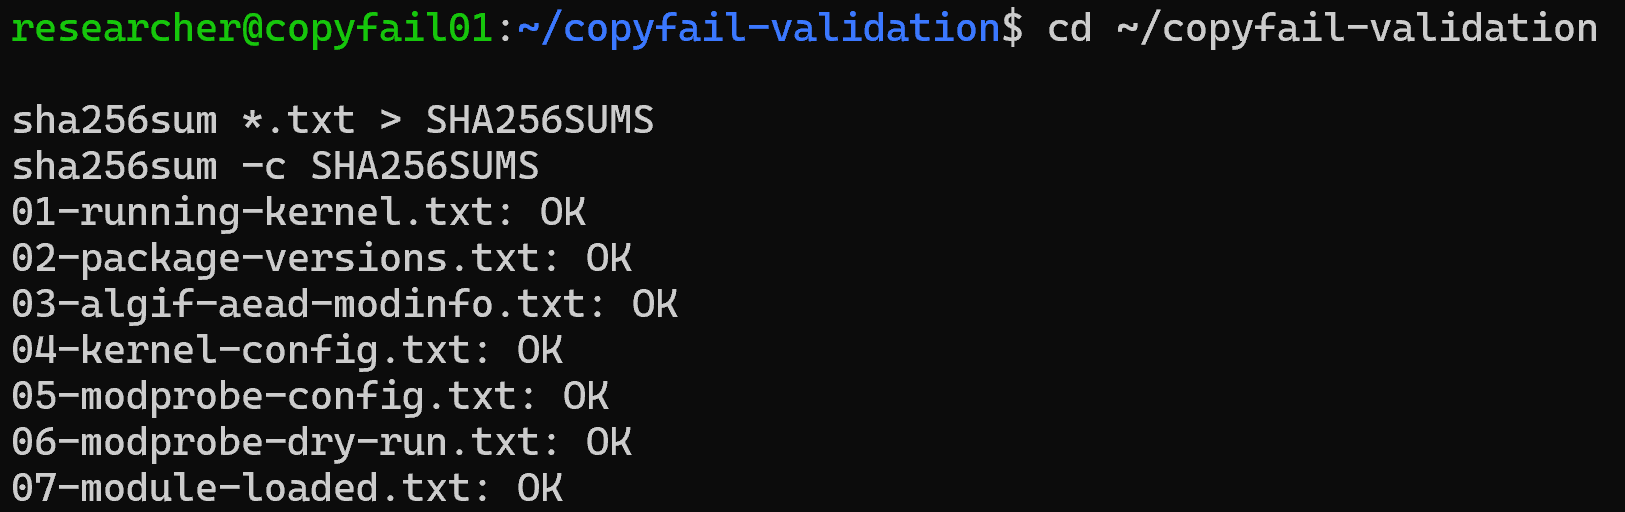
\includegraphics[
        width=\textwidth,
        height=0.46\textheight,
        keepaspectratio
    ]{01-vulnerability-validation/screenshots/01-validation-integrity-check.png}
    \caption{Phase~01 command-output files verified against their recorded
    SHA-256 list. This capture illustrates the integrity check used around the
    experimental evidence packages.}
    \label{fig:phase01-evidence-integrity-check}
\end{figure}

Manifest scope was defined per package. The manifest was excluded from its own
coverage, while editable documentation could be included or explicitly
excluded according to the phase. A file beside
\code{PUBLIC-SHA256SUMS.txt} was therefore not automatically covered;
verification used the manifest's enumerated paths. A filename or object change
after manifest generation invalidated that entry until the manifest was updated.
Verification results were therefore recorded entry by entry rather than
summarized from the mere presence of a manifest.

SHA-256 verification was a change-detection mechanism, not proof that a capture
was complete or correctly interpreted. A matching digest shows that the checked
bytes correspond to the listed version. It does not establish when a command
ran, whether it captured the intended property, whether a screenshot omitted
context, or whether documentation describes the artifact accurately. Content
review and cryptographic verification were separate publication gates.

The public copy was reviewed for credentials, tokens, internal network details,
machine identifiers, and unrelated environmental information. Exploit source
or other unnecessary material could be withheld while retaining hashes,
provenance, system state, and execution outcomes. Omissions were documented,
numbering gaps were preserved where useful, and publication edits did not
overwrite the unsanitized original.

Incomplete captures were retained and described according to their contents. A
failed text capture stayed failed even when a contemporaneous screenshot
preserved the missing result. The screenshot could supplement the record, but
it did not rewrite the status of the original artifact. Screenshot-only runs
also remained screenshot-only; no replacement transcript was created after the
fact.

This workflow supports internal traceability and change detection, but is not a
formal forensic acquisition with an independent trusted timestamp,
hardware-backed attestation, or external witness. Later claims are therefore
limited to the properties preserved by the cited artifacts and to the
controlled laboratory states in which they were collected.
  \clearpage
  \section{Clean Baseline}
\label{sec:clean-baseline}

\subsection{Purpose and Evidence Scope}

Before any Copy Fail-specific testing began, VM~270
\code{copyfail01} was recorded as the reference system. This was the state
against which later kernel, package, configuration, target-file, and privilege
changes could be compared. Preserving it separately also meant that the
vulnerable reconstruction on VM~271 did not overwrite the known starting
point.

Here, \emph{clean} describes a position in the experimental sequence. It means
that no vulnerability-specific configuration, proof-of-concept execution, or
exploitation had yet been introduced within the documented workflow. It does
not mean that every security property of the guest had already been tested, or
that the installed kernel could be classified as vulnerable or protected from
the baseline alone. Chapter~4 performs that narrower validation.

\begin{evidencebox}
The public guest-state evidence is stored under
\path{evidence/00-baseline/}. It contains 20 command-output artifacts, a
private-origin manifest, and a separate manifest for the sanitized public
copy. The reviewed Phase~00 screenshot directory contains no retained image,
so this chapter uses the machine-readable captures directly instead of
presenting a later-phase screenshot as baseline evidence.
\end{evidencebox}

The baseline covers the operating-system identity, active kernel, installed
packages, available upgrades, account state, network configuration, listening
sockets, and storage layout. A separate Proxmox transcript records the virtual
hardware and snapshot state. Together, the guest and hypervisor views establish
which machine was recorded and which checkpoint later experiments used as
their reference.

\subsection{Operating-System and Account State}

The guest identified itself as \code{copyfail01}, running Ubuntu 24.04.2 LTS
on x86-64 KVM/QEMU hardware. The relevant sanitized excerpt from
\path{command-output/hostnamectl.txt} is reproduced below.

\begin{lstlisting}
Static hostname: copyfail01
Chassis: vm
Virtualization: kvm
Operating System: Ubuntu 24.04.2 LTS
Kernel: Linux 6.8.0-137-generic
Architecture: x86-64
Hardware Vendor: QEMU
Hardware Model: Standard PC _Q35 + ICH9, 2009_
\end{lstlisting}

\Cref{tab:baseline-system-identity} combines that guest view with the
non-sensitive fields retained from the later hypervisor verification.

\begin{table}[H]
    \centering
    \caption{Recorded identity of the reference guest.}
    \label{tab:baseline-system-identity}
    \small
    \begin{tabularx}{0.92\textwidth}{@{}>{\bfseries}p{0.31\textwidth}Y@{}}
        \toprule
        Property & Recorded state \\
        \midrule
        Hypervisor object &
        Proxmox VM~270, configured as \code{copyfail01} \\

        Guest hostname &
        \code{copyfail01} \\

        Operating system &
        Ubuntu 24.04.2 LTS (Noble Numbat) \\

        Architecture &
        \code{x86-64} \\

        Virtual platform &
        KVM guest on QEMU Q35 hardware with UEFI firmware \\

        Administrative account &
        \code{researcher}, UID~1000 and GID~1000 \\
        \bottomrule
    \end{tabularx}
\end{table}

The matching hypervisor name and guest hostname link the command-output set to
the intended VM without depending on only one naming source. The
\code{id.txt} capture also records the baseline administrative account as
\code{researcher}, including membership in \code{adm}, \code{sudo}, and
\code{lxd}. This account was used for preparation and evidence collection; it
was not the unprivileged attacker identity used for the vulnerable
reproduction.

Machine and boot identifiers were redacted from the publication copy. Those
values are unnecessary for interpreting the experiment, while the hostname,
release, architecture, and virtualization fields retain the system identity
needed for comparison.

\subsection{Kernel and Package State}

Three runtime captures independently report the same active kernel release:
\path{kernel.txt}, \path{uname.txt}, and \path{proc-version.txt}. The package
database then links that active release to the installed Ubuntu image package.
This matters because an installed image does not prove which kernel is running,
and a runtime release string does not preserve the corresponding package
version.

\begin{lstlisting}
$ cat command-output/kernel.txt
6.8.0-137-generic

$ cat command-output/kernel-packages.txt
linux-image-6.8.0-137-generic    6.8.0-137.137
linux-image-generic              6.8.0-137.137

$ cat command-output/kernel-sha256.txt
76a7f2ef15fcbd2f5c25cd7e7b413f903b2078396063557f1dffb4a0b089a964  /boot/vmlinuz-6.8.0-137-generic
\end{lstlisting}

\begin{table}[H]
    \centering
    \caption{Recorded kernel state of VM~270.}
    \label{tab:baseline-kernel-state}
    \small
    \begin{tabularx}{\textwidth}{@{}>{\bfseries}p{0.29\textwidth}Y@{}}
        \toprule
        Property & Recorded state \\
        \midrule
        Running release &
        \code{6.8.0-137-generic} \\

        Kernel build &
        \code{\#137-Ubuntu SMP PREEMPT\_DYNAMIC}, built 17 July 2026 at
        20:28:23 UTC \\

        Installed image &
        \code{linux-image-6.8.0-137-generic}, version
        \code{6.8.0-137.137} \\

        Tracking package &
        \code{linux-image-generic}, version \code{6.8.0-137.137} \\

        Image architecture &
        \code{amd64} \\

        Recorded image digest &
        Captured in \path{command-output/kernel-sha256.txt} and reproduced
        in the evidence excerpt above \\
        \bottomrule
    \end{tabularx}
\end{table}

The digest identifies the kernel image that was present when the capture was
made. Because the image itself is not part of the public evidence set, the
digest cannot be recalculated from the repository alone. Manifest verification
confirms the integrity of the retained digest record, not the bytes of the
unpublished \code{vmlinuz} file.

The complete package inventory contains 680 package rows. The separate
\code{upgradable.txt} capture contains 77 package entries after excluding the
\code{apt} warning and heading lines. Those updates were recorded but not
applied before the baseline checkpoint.

\begin{table}[H]
    \centering
    \caption{Selected package facts relevant to later experimental work.}
    \label{tab:baseline-package-state}
    \small
    \begin{tabularx}{\textwidth}{@{}>{\bfseries\raggedright\arraybackslash}p{0.23\textwidth}>{\raggedright\arraybackslash}p{0.29\textwidth}Y@{}}
        \toprule
        Category & Recorded item & Baseline state \\
        \midrule
        Inventory scope &
        Installed packages &
        680 package rows with retained versions \\

        Pending changes &
        Upgradable packages &
        77 package rows; updates not applied before the checkpoint \\

        Kernel support &
        \code{kmod}; \code{initramfs-tools} &
        Versions \code{31+20240202-2ubuntu7.2} and
        \code{0.142ubuntu25.4} \\

        Existing observability &
        \code{bpfcc-tools}; \code{bpftrace}; \code{linux-tools-common} &
        Versions \code{0.29.1+ds-1ubuntu7},
        \code{0.20.2-1ubuntu4.3}, and \code{6.8.0-137.137} \\

        General tooling &
        \code{git}; \code{python3} &
        Versions \code{1:2.43.0-1ubuntu7.3} and
        \code{3.12.3-0ubuntu2.1} \\

        Exact build-tool entries &
        \code{build-essential}; \code{gcc}; \code{g++}; \code{clang};
        \code{make}; \code{bpftool}; \code{libbpf-dev} &
        No exact package row for these names in the captured inventory \\
        \bottomrule
    \end{tabularx}
\end{table}

The final row is intentionally narrow. Supporting components including
\code{gcc-14-base:amd64}, \code{libclang1-18}, and
\code{libclang-cpp18} were installed, so the evidence does not support the
broader claim that the system contained no GCC- or Clang-related packages. It
supports only the absence of the exact build-tool package names listed in the
table. Package presence also does not prove that a detector was executed, just
as package absence does not prove that no binary could have been transferred
to the guest.

\subsection{Network State}

The network baseline was recorded from both sides of the VM boundary. Proxmox
assigned VM~270 one VirtIO interface on \code{vmbr1} with firewall processing
enabled. Inside the guest, the corresponding interface appeared as
\code{enp6s18}; no second non-loopback interface appears in the captured address
state.

Netplan configured the interface for DHCP. The runtime route capture shows a
connected laboratory-subnet route and a default route through the laboratory
gateway. Concrete addresses and the MAC value were sanitized, while the
interface, addressing method, and routing role were retained.

\begin{lstlisting}
network:
  version: 2
  ethernets:
    enp6s18:
      dhcp4: true

default via <LAB_GATEWAY> dev enp6s18 proto dhcp src <LAB_VM_IP>
<LAB_SUBNET> dev enp6s18 proto kernel scope link src <LAB_VM_IP>
\end{lstlisting}

The listening-socket capture records SSH on TCP port~22 for IPv4 and IPv6,
plus the local \code{systemd-resolved} stub listeners on loopback port~53. No
other listener appears in that capture. This is a point-in-time result, not a
claim that the same listener set persisted through every later phase.

Together, the hypervisor and guest records match the topology from Chapter~2:
the Copy Fail guest used the isolated \code{vmbr1} segment and reached routed
destinations through the laboratory gateway rather than through a direct
management-network attachment.

\subsection{Storage State}

Proxmox presented a single 32~GiB virtual disk through VirtIO SCSI, with
discard, an I/O thread, and the virtual SSD flag enabled. The guest reported
the same capacity as \code{/dev/sda}. Its recorded layout is summarized in
\cref{tab:baseline-storage-state}.

\begin{table}[H]
    \centering
    \caption{Recorded storage layout and utilisation.}
    \label{tab:baseline-storage-state}
    \small
    \begin{tabularx}{\textwidth}{@{}>{\bfseries}p{0.27\textwidth}Y@{}}
        \toprule
        Component & Recorded state \\
        \midrule
        Virtual disk &
        One 32~GiB disk, visible inside the guest as \code{/dev/sda} \\

        EFI partition &
        \code{/dev/sda1}, 1~GiB VFAT, mounted at \code{/boot/efi} \\

        Boot partition &
        \code{/dev/sda2}, 2~GiB ext4, mounted at \code{/boot} \\

        LVM partition &
        \code{/dev/sda3}, 28.9~GiB, assigned to \code{ubuntu-vg} \\

        Root logical volume &
        \code{ubuntu-lv}, 14.47~GiB ext4, mounted at \code{/} \\

        Free LVM space &
        Approximately 14.47~GiB \\

        Root utilisation &
        15~GiB reported size, 5.6~GiB used, 7.9~GiB available,
        42\% utilisation \\
        \bottomrule
    \end{tabularx}
\end{table}

The storage capture establishes capacity and allocation before later
experiment-specific files were introduced. It does not imply that this layout
caused or prevented Copy Fail; it provides a fixed comparison point for later
file and filesystem observations.

\subsection{Integrity Verification}

The baseline uses separate SHA-256 manifests for two different byte sets. The
private manifest describes the original command output. The public manifest
describes the sanitized publication copy after machine and network identifiers
were removed. Reusing the private hashes for the modified public files would
have made legitimate redaction look like corruption, so the two states remain
explicitly separate.

An independent check of
\path{evidence/00-baseline/hashes/PUBLIC-SHA256SUMS} against the reviewed public
repository returned \code{OK} for all 20 enumerated files. The public command
output was also compared with the private-origin manifest to locate the effect
of sanitization. Seventeen files still matched; the expected mismatches were
\path{hostnamectl.txt}, \path{ip-addresses.txt}, and \path{routes.txt}.

\begin{table}[H]
    \centering
    \caption{Independent Phase~00 integrity results.}
    \label{tab:baseline-integrity-results}
    \small
    \begin{tabularx}{\textwidth}{@{}>{\bfseries\raggedright\arraybackslash}p{0.28\textwidth}>{\raggedright\arraybackslash}p{0.18\textwidth}Y@{}}
        \toprule
        Check & Result & Interpretation \\
        \midrule
        Public files against public manifest &
        20 of 20 matched &
        Every command-output object listed by the public manifest retained its
        recorded public bytes. \\

        Sanitized files against private-origin manifest &
        17 of 20 matched &
        The three mismatches correspond to the files changed by publication
        redaction. \\
        \bottomrule
    \end{tabularx}
\end{table}

The manifest scope matters. The 20 entries cover the command-output artifacts;
they do not cover the README, the manifests themselves, or every file beside
them. A successful check therefore detects changes to the listed bytes, but it
does not authenticate the origin of a command, prove that a capture was
complete, or settle a disagreement in documentation that lies outside the
manifest.

\subsection{Snapshot Verification and Baseline Result}

After the guest-state collection, Proxmox preserved VM~270 at the named
baseline checkpoint. Its exact snapshot name appears in the transcript below.
A later read-only capture, taken on 13 August 2026 at 21:53:07+02:00, found
the VM stopped and recorded both its parent field and its snapshot tree.

\begin{lstlisting}
status: stopped
cores: 2
memory: 4096
machine: q35
name: copyfail01
net0: virtio=<REDACTED_MAC>,bridge=vmbr1,firewall=1
parent: clean-baseline-00
scsi0: <REDACTED_STORAGE_ID>,discard=on,iothread=1,size=32G,ssd=1

`-> clean-baseline-00  2026-08-08 00:46:54
    Fresh Ubuntu 24.04.2 LTS Copy Fail research target.
 `-> current
\end{lstlisting}

The Phase~00 README calls the snapshot \code{00-clean-baseline}. That name does
not match the Proxmox evidence. Both the hypervisor parent field and the
snapshot listing use \code{clean-baseline-00}, so this chapter treats that as
the authoritative snapshot name. The README is not one of the 20 files covered
by the public command-output manifest, which is why the successful manifest
check does not resolve or conceal this documentation mismatch.

The snapshot listing records its creation time as 8 August 2026 at 00:46:54
and does not include a timezone. None is assigned here. The later transcript
does prove that the snapshot existed, that VM~270's then-current state descended
from it, and that the VM was stopped when the verification was collected. It
does not independently prove the content of an unexported virtual disk or every
historical action performed inside the guest.

At the end of this chapter, the experiment therefore has a concrete reference
state: Ubuntu 24.04.2 LTS on kernel \code{6.8.0-137-generic}, a documented
package and account inventory, one isolated laboratory interface, a recorded
storage layout, 20 publicly verifiable command-output artifacts, and a confirmed
Proxmox rollback point. That is enough to compare later state changes without
turning the word \emph{clean} into an unsupported security verdict.

Chapter~4 next checks \code{algif\_aead} availability, the effective loading
policy, and the kernel's patch state before VM~271 is modified.
  \clearpage
  \section{Vulnerability Analysis and Reference-System Validation}
\label{sec:reference-validation}

\graphicspath{{../evidence/}{evidence/}}

Chapter~3 established VM~270 \code{copyfail01} as the clean reference system.
That baseline answers what was installed and running, but it does not answer the
next question: could this exact state reproduce Copy Fail? A 6.8-series kernel,
the AF\_ALG subsystem, or an \code{algif\_aead} file on disk is not enough on
its own. The interface must be supported, reachable at runtime, and backed by a
kernel that still contains the vulnerable behaviour.

This chapter checks those conditions without running the proof of concept on
VM~270. That boundary is deliberate. If the reference system is already
protected, downgrading it or removing its mitigation would destroy the most
useful comparison state in the laboratory. The result of this analysis therefore
decides whether VM~270 can be used directly or whether the vulnerable state has
to be reconstructed on the separate experimental clone, VM~271.

\begin{evidencebox}
Phase~01 is stored under
\path{evidence/01-vulnerability-validation/}. The public set contains seven
text artifacts and seven screenshots. An independent check of
\path{PUBLIC-SHA256SUMS} verified all 14 listed objects with no failures. The
machine-readable captures remain the primary evidence; selected screenshots are
included here to make the decisive states visible in the report.
\end{evidencebox}

\subsection{Validation Question and Method}

The validation was organised around five separate questions:

\begin{enumerate}
    \item Does the installed kernel provide the \code{algif\_aead} module?
    \item Is the AF\_ALG AEAD userspace interface enabled in the running
          kernel's configuration?
    \item Was \code{algif\_aead} loaded when the evidence was collected?
    \item What does the ordinary \code{modprobe} path do when the module is
          requested?
    \item Is the active Ubuntu kernel before or after Canonical's published
          fixed-package boundary?
\end{enumerate}

Keeping these questions separate prevents several misleading shortcuts. A
module can exist without being loaded. Kernel support can be configured while a
distribution policy blocks normal loading. Even a reachable interface does not
establish vulnerability if the active implementation is already corrected.
Suitability for reproduction depends on the combined state, not on a single
command or version string.

The seven textual artifacts record the running kernel, relevant package
versions, module metadata, kernel configuration, effective loading policy, and
runtime module state. They are interpreted below in that order. No exploit was
executed on VM~270 during this phase, so the result is a prerequisite assessment
rather than an exploit-success or exploit-failure experiment.

\clearpage

\subsection{Module Object and Kernel Configuration}

The capture in \path{03-algif-aead-modinfo.txt} shows that the running kernel's
module tree contains \code{algif\_aead}:

\begin{lstlisting}
filename: /lib/modules/6.8.0-137-generic/kernel/crypto/algif_aead.ko.zst
description: AEAD kernel crypto API user space interface
depends: af_alg
intree: Y
name: algif_aead
vermagic: 6.8.0-137-generic SMP preempt mod_unload modversions
\end{lstlisting}

The filename and \code{vermagic} associate the object with the active
\code{6.8.0-137-generic} release. Its description identifies the AEAD
userspace interface relevant to Copy Fail, while the dependency on
\code{af\_alg} matches the AF\_ALG path described in Chapter~1.

The corresponding configuration capture in \path{04-kernel-config.txt}
contains:

\begin{lstlisting}
CONFIG_CRYPTO_USER_API=m
CONFIG_CRYPTO_USER_API_HASH=m
CONFIG_CRYPTO_USER_API_SKCIPHER=m
CONFIG_CRYPTO_USER_API_RNG=m
# CONFIG_CRYPTO_USER_API_RNG_CAVP is not set
CONFIG_CRYPTO_USER_API_AEAD=m
# CONFIG_CRYPTO_USER_API_ENABLE_OBSOLETE is not set
\end{lstlisting}

The decisive entry is \code{CONFIG\_CRYPTO\_USER\_API\_AEAD=m}. The value
\code{m} means that this userspace AEAD interface is available as a loadable
module rather than omitted or built directly into the kernel. This agrees with
the module object reported by \code{modinfo}.

\begin{figure}[H]
    \centering
    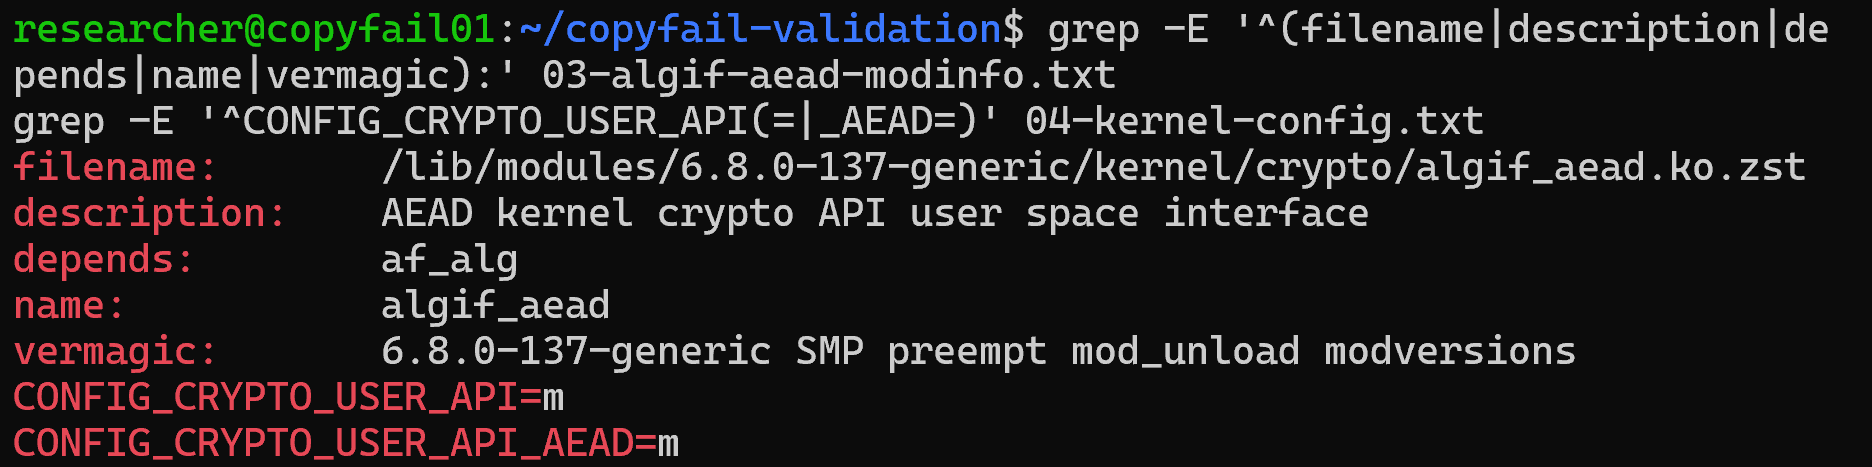
\includegraphics[
        width=\textwidth,
        height=0.31\textheight,
        keepaspectratio
    ]{01-vulnerability-validation/screenshots/04-algif-aead-module-and-kernel-config.png}
    \caption{Phase~01 capture linking the installed \code{algif\_aead} object
    to the active kernel and showing modular AEAD userspace support.}
    \label{fig:phase01-module-config}
\end{figure}

These observations establish installed capability only. Neither \code{modinfo}
nor the kernel configuration proves that the module was loaded, that the normal
loading path would permit it, or that its implementation remained vulnerable.
Those properties require the runtime, policy, and package checks that follow.

\subsection{Runtime Module State}

The loaded-module list was checked with an exact-name query:

\begin{lstlisting}
lsmod | grep '^algif_aead\b'
\end{lstlisting}

The command returned no output. For that reason,
\path{07-module-loaded.txt} is exactly zero bytes; it is not a missing capture.
Its manifest entry uses the standard SHA-256 digest of an empty file:

\begin{lstlisting}
e3b0c44298fc1c149afbf4c8996fb92427ae41e4649b934ca495991b7852b855  07-module-loaded.txt
\end{lstlisting}

The accompanying screenshot uses a human-readable conditional wrapper and
prints \code{algif\_aead is NOT currently loaded}. It presents the same point-in-
time result without replacing the machine-readable empty artifact.

\begin{figure}[H]
    \centering
    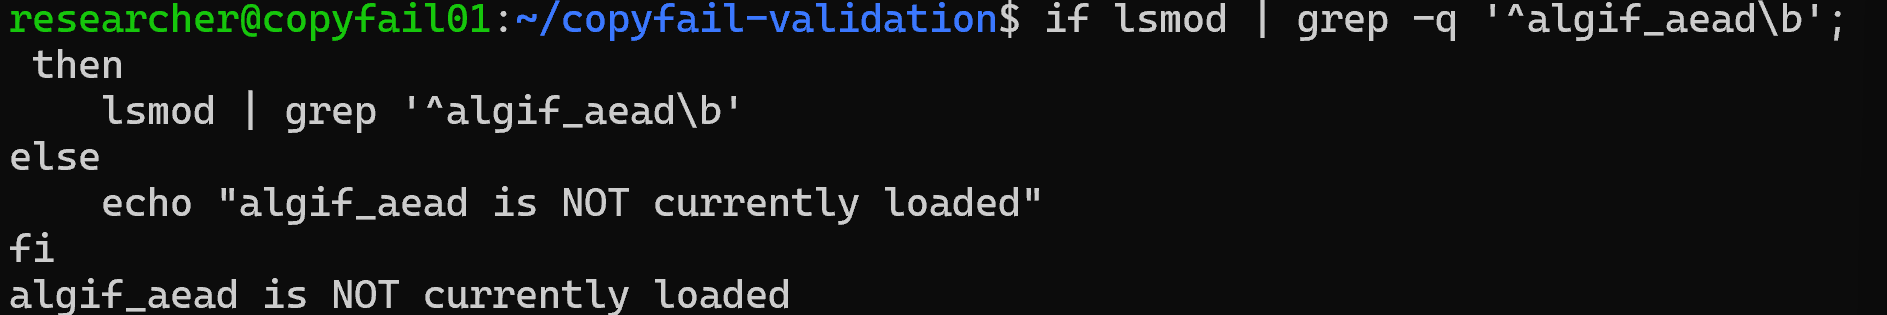
\includegraphics[
        width=\textwidth,
        height=0.29\textheight,
        keepaspectratio
    ]{01-vulnerability-validation/screenshots/05-algif-aead-not-loaded.png}
    \caption{Runtime check showing that \code{algif\_aead} was not loaded at
    the Phase~01 collection point.}
    \label{fig:phase01-module-unloaded}
\end{figure}

This result is intentionally narrow. It proves that the module did not appear
in the loaded-module list at that moment. By itself, it cannot distinguish a
module that had simply not been requested from one whose loading was actively
blocked. The effective policy check supplies that missing context.

\subsection{Effective Module-Loading Policy}

The capture in \path{05-modprobe-config.txt} found the following rule:

\begin{lstlisting}
/etc/modprobe.d/disable-algif_aead.conf:1:# Disable algif_aead module due to CVE-2026-31431 (AKA copy.fail)
/etc/modprobe.d/disable-algif_aead.conf:5:install algif_aead /bin/false
\end{lstlisting}

For \code{modprobe}, the \code{install} directive replaces normal insertion of
the named module with the specified command. Here, a request for
\code{algif\_aead} is redirected to \code{/bin/false}, which exits
unsuccessfully without inserting the module. Canonical documents the same
\code{kmod}-based rule as a temporary Copy Fail mitigation
\cite{ubuntu-copyfail-cve,ubuntu-copyfail-fixes}.

The configuration was not interpreted from the file alone. The effective path
was resolved with a dry run and preserved in
\path{06-modprobe-dry-run.txt}:

\begin{lstlisting}
insmod /lib/modules/6.8.0-137-generic/kernel/crypto/af_alg.ko.zst
install /bin/false
\end{lstlisting}

The first line resolves the \code{af\_alg} dependency. The second shows that
the requested \code{algif\_aead} insertion resolves to the replacement command
instead of an \code{insmod} operation.

\begin{figure}[H]
    \centering
    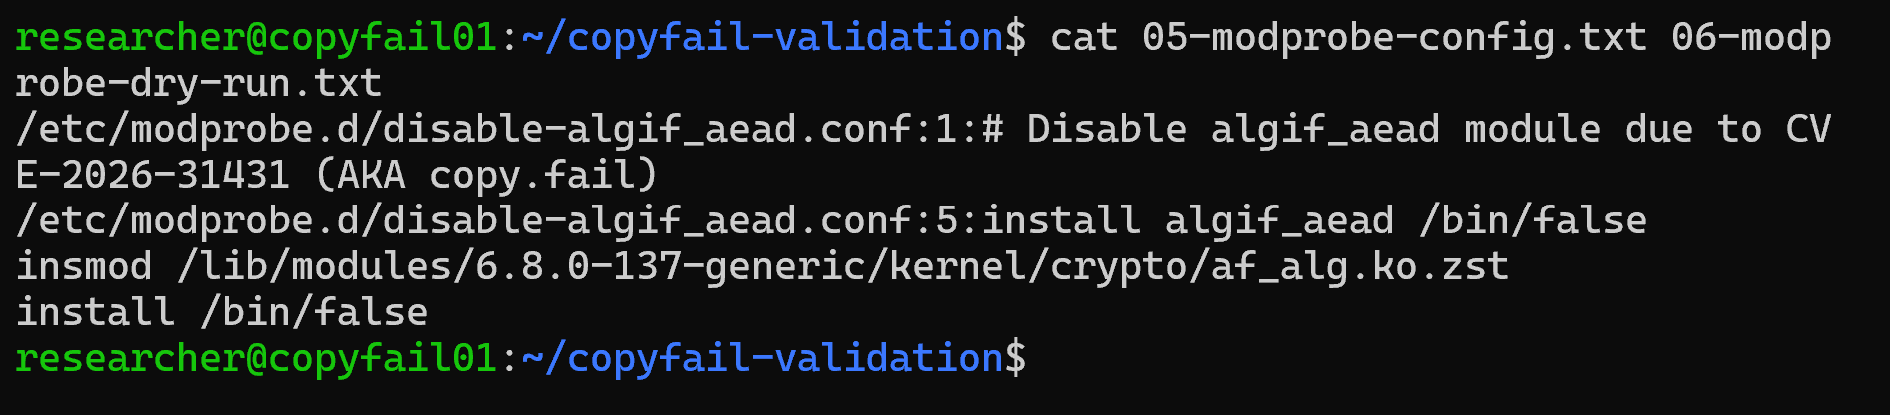
\includegraphics[
        width=\textwidth,
        height=0.31\textheight,
        keepaspectratio
    ]{01-vulnerability-validation/screenshots/03-algif-aead-mitigation-active.png}
    \caption{Configuration and dry-run output showing the active
    \code{algif\_aead} rule on the ordinary \code{modprobe} path.}
    \label{fig:phase01-mitigation-policy}
\end{figure}

Because \code{modprobe -n -v} is a dry run, it resolves the selected actions
without executing them. The evidence therefore establishes the behaviour of
the ordinary distribution loading path used by this laboratory procedure. It
does not claim that every possible low-level mechanism for introducing kernel
code was tested. The policy content and its resolution are stronger evidence
for this conclusion than the installed \code{kmod} version alone.

\subsection{Kernel and Package Boundary}

The runtime capture reports \code{6.8.0-137-generic}. The package capture links
that release to the installed Noble generic-kernel packages:

\begin{lstlisting}
kmod                              31+20240202-2ubuntu7.2
linux-image-6.8.0-137-generic     6.8.0-137.137
linux-image-generic               6.8.0-137.137
\end{lstlisting}

\begin{figure}[H]
    \centering
    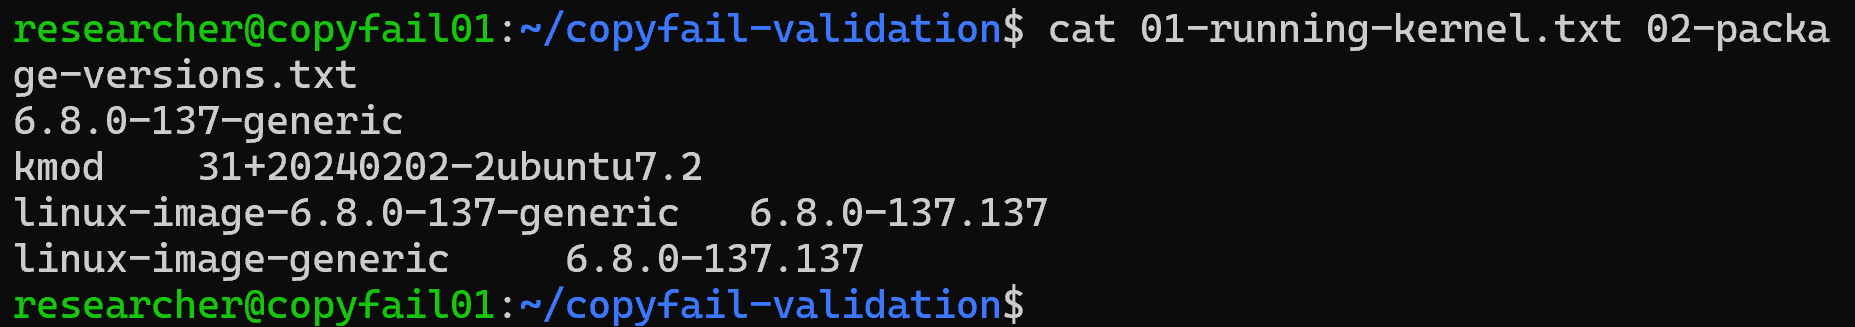
\includegraphics[
        width=\textwidth,
        height=0.29\textheight,
        keepaspectratio
    ]{01-vulnerability-validation/screenshots/02-patched-kernel-and-kmod.png}
    \caption{Running release and installed package versions recorded on
    VM~270 during Phase~01.}
    \label{fig:phase01-kernel-packages}
\end{figure}

Canonical identifies \code{6.8.0-117.117} as the first fixed version of the
Ubuntu 24.04 LTS Noble generic \code{linux} package
\cite{ubuntu-copyfail-cve}. The active \code{6.8.0-137.137} image is a later
update in that same maintained package series. VM~270 is therefore classified
as running a corrected vendor package.

This conclusion is based on the recorded runtime and package state together
with Canonical's published fixed-version boundary. It is not an independent
source-code review or binary comparison of the kernel image. That distinction
matters: the evidence supports a vendor-package classification, not a claim that
the patch was reimplemented or reverse engineered during this project.

\subsection{Combined Result}

The validation produces a layered result rather than a single yes-or-no module
check:

\begin{table}[H]
    \centering
    \caption{Copy Fail prerequisite assessment for VM~270.}
    \label{tab:reference-system-validation}
    \small
    \begin{tabularx}{\textwidth}{@{}>{\bfseries\raggedright\arraybackslash}p{0.29\textwidth}>{\raggedright\arraybackslash}p{0.17\textwidth}Y@{}}
        \toprule
        Property & Observation & What the evidence establishes \\
        \midrule
        Module object present &
        Yes &
        \code{algif\_aead.ko.zst} exists for the active release. \\

        AEAD userspace API configured &
        Yes, as a module &
        \code{CONFIG\_CRYPTO\_USER\_API\_AEAD=m} enables modular support. \\

        Module loaded at capture &
        No &
        The exact-name runtime query returned no row. \\

        Ordinary loading path permitted &
        No &
        \code{modprobe} resolves the requested insertion to
        \code{/bin/false}. \\

        Active kernel before fixed boundary &
        No &
        \code{6.8.0-137.137} is within the same Noble generic series and later
        than Canonical's fixed version, \code{6.8.0-117.117}. \\

        Suitable for direct reproduction &
        No &
        The captured reference state has both a module-loading control and a
        vendor-classified corrected kernel. \\
        \bottomrule
    \end{tabularx}
\end{table}

The module object and kernel support are present, but presence is not the same
as reachability or vulnerability. At collection time the module was unloaded,
the normal loading path was blocked, and the active kernel package was already
past the published correction boundary. VM~270 is therefore a protected
reference system, not a valid direct reproduction target.

No proof of concept was run on VM~270, so this chapter does not report an
observed exploit failure. Its conclusion is narrower and better supported: the
captured machine does not satisfy the prerequisites selected for the controlled
reproduction. Later protected-state retests remain separate experiments.

\subsection{Preserving the Reference System}

VM~270 was kept in its reference role instead of being downgraded or having its
module policy removed. Chapter~3 records the corresponding Proxmox state: the
machine was stopped and the current state descended from the
\code{clean-baseline-00} snapshot at the verification point. Preserving that
state keeps three later comparisons meaningful: vulnerable behaviour on
VM~271, behaviour under compensating controls, and behaviour after the vendor
kernel correction.

This also keeps experimental changes on the machine created for them. VM~271
\code{copyfail-vuln} is the clone on which the vulnerable kernel, necessary
module-policy change, proof of concept, detector, and compensating controls are
introduced. Its cloned machine identifiers and SSH host keys must be regenerated
before use, as specified in Chapter~2.

\subsection{Requirements for the Vulnerable Clone}

The reference-system result defines what must be shown on VM~271 before any
proof-of-concept execution:

\begin{table}[H]
    \centering
    \caption{Pre-reproduction acceptance criteria for VM~271.}
    \label{tab:vulnerable-clone-requirements}
    \small
    \begin{tabularx}{\textwidth}{@{}>{\bfseries\raggedright\arraybackslash}p{0.30\textwidth}Y@{}}
        \toprule
        Requirement & Evidence required before reproduction \\
        \midrule
        Candidate vulnerable kernel &
        Record the running release and exact installed image, module, and
        metapackage versions. \\

        Module mitigation absent or disabled &
        Capture the relevant \code{modprobe.d} content and the effective
        \code{modprobe -n -v algif\_aead} resolution. \\

        Affected interface reachable &
        Confirm that \code{algif\_aead} exists, can be loaded, and exposes the
        AF\_ALG AEAD path required by the reproduction. \\

        Unprivileged test identity &
        Record \code{labuser}, its UID and groups, and the absence of existing
        administrative privilege. \\

        Clean target state &
        Record the ownership, mode, size, and SHA-256 digest of the selected
        SUID target before execution. \\

        Isolation and identity separation &
        Keep the guest on the isolated laboratory network and regenerate the
        identifiers inherited during cloning. \\

        Recoverable checkpoint &
        Preserve a pre-PoC snapshot and its associated evidence before the
        exploit is introduced or executed. \\
        \bottomrule
    \end{tabularx}
\end{table}

Kernel package \code{6.8.0-116.116} was selected as the reconstruction
candidate because it immediately precedes Canonical's first fixed Noble generic
version, \code{6.8.0-117.117}. That ordering identifies a candidate package;
it does not by itself prove that the guest booted it, exposed the required
interface, or reproduced the vulnerability. Those points require direct runtime
and experimental evidence from VM~271.

Chapter~5 therefore begins by validating that reconstructed runtime and the
clean pre-exploitation state. Only after those checks can a privilege change be
attributed to the intended Copy Fail experiment rather than to an unknown
kernel, an already modified target, or an account with pre-existing privilege.
  \clearpage
  \section{Vulnerable Reconstruction and Controlled Reproduction}
\label{sec:controlled-reproduction}

\graphicspath{{../evidence/}{evidence/}}

Chapter~4 established that VM~270 was already protected and could not serve as
the direct reproduction target. The active kernel was beyond Canonical's fixed
package boundary, and the ordinary \code{modprobe} path for
\code{algif\_aead} was blocked. VM~270 therefore remained the reference
system. The vulnerable state was reconstructed on VM~271
\code{copyfail-vuln}, the separate experimental clone created for this phase.

The reconstruction used Ubuntu kernel \code{6.8.0-116-generic}, supplied by
package version \code{6.8.0-116.116}. Before the preserved execution, the
running kernel, package state, module-loading path, test identity, and selected
SUID target were recorded. The proof of concept was then launched from
\code{labuser}, UID~1001. Success was defined by the resulting process
reporting UID~0, not by a changed prompt or file digest alone.

A preliminary run had already been used to explore the behaviour of the target
file. Because that run changed the byte stream returned through the mounted
path, VM~271 was rebooted into the same vulnerable kernel before the preserved
sequence began. The final run therefore starts from a restored observable
target state instead of presenting an already modified system as clean.

No persistence, credential collection, lateral movement, reverse shell, or
unrelated post-exploitation activity was performed. The chapter follows the
experiment only as far as necessary to establish the UID transition, compare
the two observed file-access paths, and record recovery after reboot.

\begin{evidencebox}
Phase~02 is stored under \path{evidence/02-reproduction/}. Its manifest lists
12 objects: five text artifacts, six screenshots, and the phase README. All 11
experimental captures verify against \path{PUBLIC-SHA256SUMS}; only the listed
\path{README.md} digest is stale. The README is therefore used as supporting
documentation, not as an integrity-verified experimental object. Screenshot
ID~04 remains intentionally absent because it exposed the complete
proof-of-concept source.
\end{evidencebox}

\subsection{Experimental Boundary and Evidence Sequence}

The evidence set contains two related but distinct sequences. The preliminary
investigation is represented by
\path{artifacts/copyfail-confirmed-vulnerable-state.txt}. It records the
intended historical kernel and package versions, the required modules in the
loaded state, and a mounted-view target digest that had already changed. That
artifact is useful for confirming the reconstructed runtime, but it cannot be
used as the clean before-state for the final execution.

VM~271 was therefore rebooted before the preserved run. It returned to
\code{6.8.0-116-generic}, and the normal mounted path for
\code{/usr/bin/su} again produced the original comparison digest:

\begin{lstlisting}
c74311fe5636b7d7f9a56239fa8adeeab12ba86fe7d41b91afa85bf9bbdae78b  /usr/bin/su
\end{lstlisting}

Here, \emph{restored observable state} means that the same vulnerable kernel
was active and the selected target again matched its recorded metadata and
mounted-view digest. It does not claim that every byte or item of volatile VM
state was compared with the original clone.

The retained evidence then follows the order shown in
\cref{tab:phase02-sequence}.

\begin{table}[H]
    \centering
    \caption{Preserved Phase~02 evidence sequence.}
    \label{tab:phase02-sequence}
    \small
    \begin{tabularx}{\textwidth}{@{}>{\bfseries}p{0.07\textwidth}>{\raggedright\arraybackslash}p{0.25\textwidth}Y@{}}
        \toprule
        ID & Preserved form & Role in the experiment \\
        \midrule
        01 & Text and screenshot &
        Records the vulnerable kernel, UID~1001 test account, SUID target, and
        original target digest before execution. \\

        02 & Screenshot &
        Records \code{algif\_aead} and \code{af\_alg} in the loaded state
        used for the reproduction. \\

        03 & Screenshot &
        Records proof-of-concept execution, the UID~0 shell, and the changed
        digest returned through the mounted target path. \\

        04 & Intentionally omitted &
        The original screenshot exposed the complete proof-of-concept source
        and is not part of the public package. \\

        05 & Text and screenshot &
        Records the return to UID~1001 while the changed mounted-view digest
        remained observable. \\

        06 & Text and screenshot &
        Compares the mounted/VFS digest with a direct read from the backing
        ext4 filesystem. \\

        07 & Text and screenshot &
        Records the original mounted-view digest after rebooting into the same
        vulnerable kernel. \\
        \bottomrule
    \end{tabularx}
\end{table}

The absent ID~04 remains in the numbering so the public files still match the
original collection order. IDs~02 and~03 are screenshot-only records; the other
retained steps also have machine-readable text. That difference matters. The
manifest verifies the published screenshot bytes, but it cannot turn a terminal
image into independently executable output or recreate the omitted source.

\subsection{Reconstructed Runtime and Clean Starting State}

The preliminary runtime capture reports the following active release and
matching package versions:

\begin{lstlisting}
6.8.0-116-generic
linux-image-6.8.0-116-generic          6.8.0-116.116
linux-modules-6.8.0-116-generic        6.8.0-116.116
linux-modules-extra-6.8.0-116-generic  6.8.0-116.116
\end{lstlisting}

The agreement between the booted release and the installed image and module
packages shows that the historical kernel was not merely present beside a newer
runtime. It was the kernel active during the experiment. Version
\code{6.8.0-116.116} is immediately before Canonical's first corrected Noble
generic package, \code{6.8.0-117.117} \cite{ubuntu-copyfail-cve}. The later
execution provides the behavioural confirmation that this reconstructed state
remained exploitable under the laboratory conditions.

Evidence item~01 was captured at \code{2026-08-08 23:02:32 UTC}, after the
reboot and before the final proof-of-concept execution. It records:

\begin{table}[H]
    \centering
    \caption{Observable starting state of the preserved run.}
    \label{tab:phase02-pre-exploit-state}
    \small
    \begin{tabularx}{\textwidth}{@{}>{\bfseries\raggedright\arraybackslash}p{0.30\textwidth}Y@{}}
        \toprule
        Observation & Recorded value \\
        \midrule
        Running kernel & \code{6.8.0-116-generic} \\
        Test identity & \code{uid=1001(labuser)}, \code{gid=1001(labuser)} \\
        Supplementary group & \code{100(users)} \\
        Selected target & \code{/usr/bin/su} \\
        Target metadata & \code{-rwsr-xr-x root root 55680} \\
        Mounted-view digest &
        \texttt{c74311fe...bbdae78b} \\
        Loaded AF\_ALG modules & No matching rows returned \\
        \bottomrule
    \end{tabularx}
\end{table}

\begin{figure}[H]
    \centering
    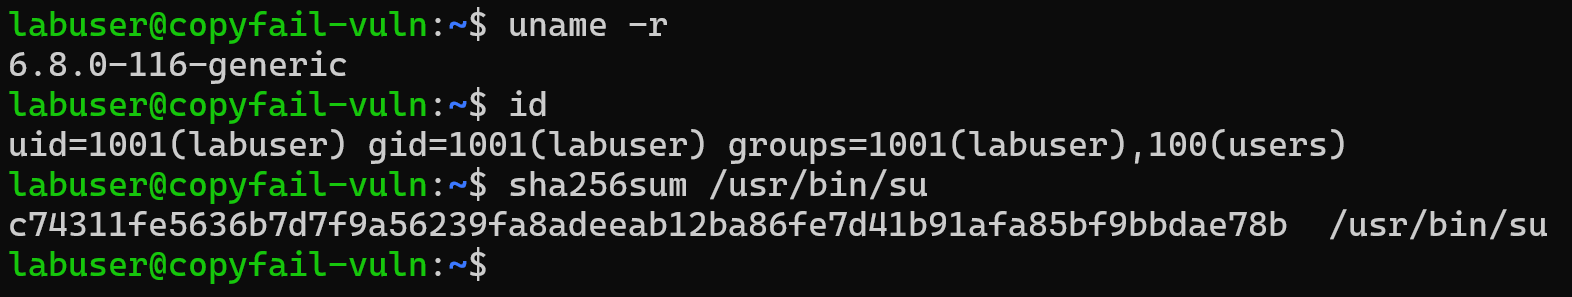
\includegraphics[
        width=\textwidth,
        height=0.25\textheight,
        keepaspectratio
    ]{02-reproduction/screenshots/01-pre-exploit-state.png}
    \caption{Interactive pre-exploitation capture showing the vulnerable
    kernel, UID~1001 test identity, and original mounted-view digest.}
    \label{fig:phase02-pre-exploit}
\end{figure}

The associated text artifact supplies the target metadata and collection time
that are not visible in the screenshot. It also records an empty exact-name
module query followed by the ordinary dry-run resolution:

\begin{lstlisting}
insmod /lib/modules/6.8.0-116-generic/kernel/crypto/af_alg.ko.zst
insmod /lib/modules/6.8.0-116-generic/kernel/crypto/algif_aead.ko.zst
\end{lstlisting}

Unlike VM~270, this path contains no \code{install /bin/false} replacement.
The empty runtime result therefore meant \emph{unloaded but normally loadable},
not absent or blocked through the tested \code{modprobe} path. The dry run did
not load either module. Evidence item~02 records the subsequent preparation
step performed by the administrative \code{researcher} account:

\begin{figure}[H]
    \centering
    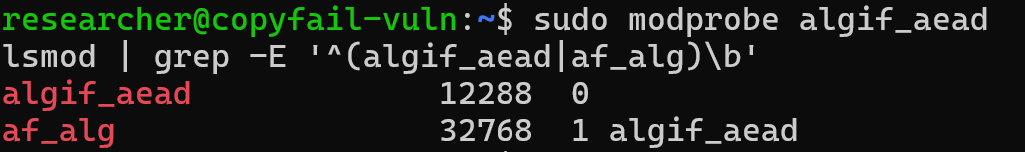
\includegraphics[
        width=\textwidth,
        height=0.20\textheight,
        keepaspectratio
    ]{02-reproduction/screenshots/02-algif-aead-loaded.png}
    \caption{Laboratory preparation step loading \code{algif\_aead} and
    recording its \code{af\_alg} dependency before exploitation.}
    \label{fig:phase02-modules-loaded}
\end{figure}

This administrative module load is not the privilege escalation. It establishes
the interface state required by the experiment, while the proof of concept was
launched separately from the \code{labuser} session. The screenshot proves the
loaded module state, not a complete AEAD encrypt/decrypt round trip.

\subsection{Proof-of-Concept Execution and UID~0 Transition}

Evidence item~03 begins at the ordinary-user prompt and records the decisive
execution sequence:

\begin{lstlisting}
labuser@copyfail-vuln:~$ python3 ~/copy_fail_exp.py
# id
uid=0(root) gid=1001(labuser) groups=1001(labuser),100(users)
# whoami
root
\end{lstlisting}

\begin{figure}[H]
    \centering
    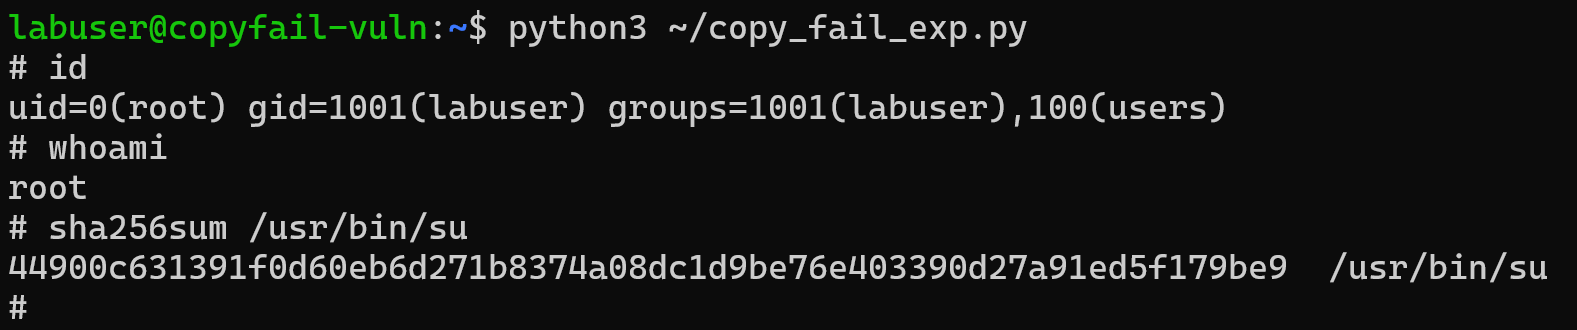
\includegraphics[
        width=\textwidth,
        height=0.28\textheight,
        keepaspectratio
    ]{02-reproduction/screenshots/03-privilege-escalation-success.png}
    \caption{Preserved execution showing the transition from the
    \code{labuser} prompt to a shell whose identity checks return UID~0 and
    \code{root}.}
    \label{fig:phase02-uid0-transition}
\end{figure}

The execution command is shown without \code{sudo}, \code{su}, or another
explicit privilege-granting wrapper. The change from a \code{\$} prompt to a
\code{\#} prompt is visually consistent with privilege, but it is not the
success criterion. The direct \code{id} and \code{whoami} results establish
the UID~0 process identity.

The process retained GID~1001 and the displayed group memberships of
\code{labuser}. The result is therefore described precisely as a transition to
UID~0, not as replacement of every credential field with the conventional root
account state. UID~0 is the trust-boundary crossing defined in Chapter~1 and is
sufficient to demonstrate local privilege escalation in this experiment.

The same screenshot records a changed SHA-256 digest for the mounted path:

\begin{lstlisting}
44900c631391f0d60eb6d271b8374a08dc1d9be76e403390d27a91ed5f179be9  /usr/bin/su
\end{lstlisting}

That changed digest is supporting behavioural evidence, not the proof of
privilege escalation. It shows that the bytes returned through the mounted path
differed from the before-state, but it does not identify the changed bytes or
prove a persistent replacement on disk.

The complete proof-of-concept source is not redistributed. Public evidence ID~04
was removed because it displayed the full source, while the numbering and
documentation retain the fact that the item existed. The Phase~02 documentation
records a 731-byte local representation and its SHA-256 digest, plus a
non-executed 732-byte trailing-newline variant. Because the README's manifest
entry is stale and item~03 does not hash the file immediately before launch,
those values are treated as documentation-level provenance rather than a
cryptographic binding between the screenshot and the exact executed bytes.

\subsection{State After Leaving the Root Shell}

Evidence item~05 was captured at \code{2026-08-08 23:24:57 UTC}, after the
UID~0 shell had been exited. The active session again reported
\code{uid=1001(labuser)} and \code{whoami} returned \code{labuser}. The target
still had the same size, owner, group, and SUID mode recorded before execution,
but its mounted-view digest remained changed.

\begin{figure}[H]
    \centering
    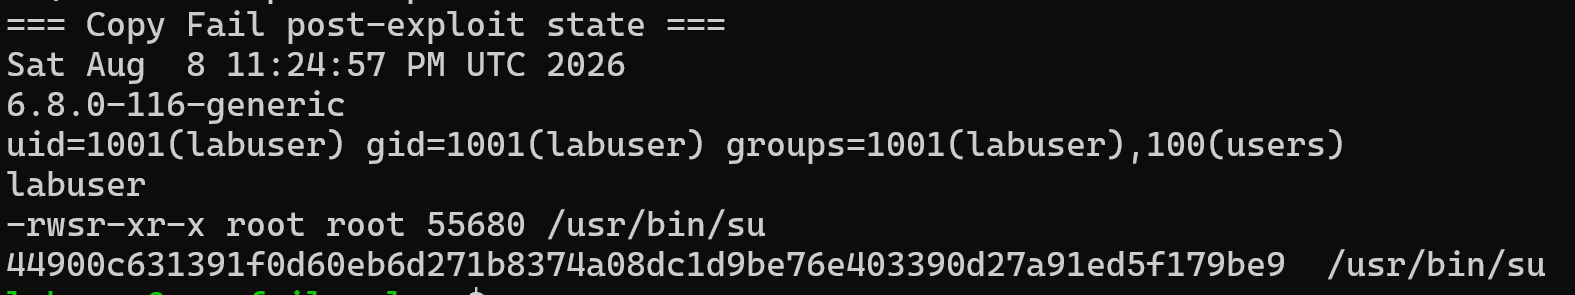
\includegraphics[
        width=\textwidth,
        height=0.26\textheight,
        keepaspectratio
    ]{02-reproduction/screenshots/05-post-exploit-state.png}
    \caption{Post-shell capture showing UID~1001 restored while the changed
    mounted-view digest remained observable.}
    \label{fig:phase02-post-exploit}
\end{figure}

Leaving the privileged shell therefore did not immediately restore the original
byte stream returned for \code{/usr/bin/su}. This does not establish persistence
in the usual security sense. No mechanism was installed to survive reboot,
retain privileged access, or automatically recreate the altered state. The
capture establishes only that the changed mounted view remained visible while
the system continued running.

The unchanged metadata also shows why a check limited to ownership, mode, and
size would not have detected the observed content difference. Conversely, a
changed digest cannot explain where the differing data resided or whether it
was ever written to persistent storage. The separate read-path comparison was
performed to answer that narrower question.

\subsection{Mounted View and Backing ext4 Read}

Evidence item~06 was captured at \code{2026-08-08 23:28:41 UTC}. The mounted
path was hashed again and compared with a direct read through \code{debugfs}
from the ext4 filesystem on the underlying logical volume:

\begin{lstlisting}
sudo debugfs -R 'cat /usr/bin/su' \
  /dev/mapper/ubuntu--vg-ubuntu--lv 2>/dev/null \
  | sha256sum
\end{lstlisting}

\begin{figure}[H]
    \centering
    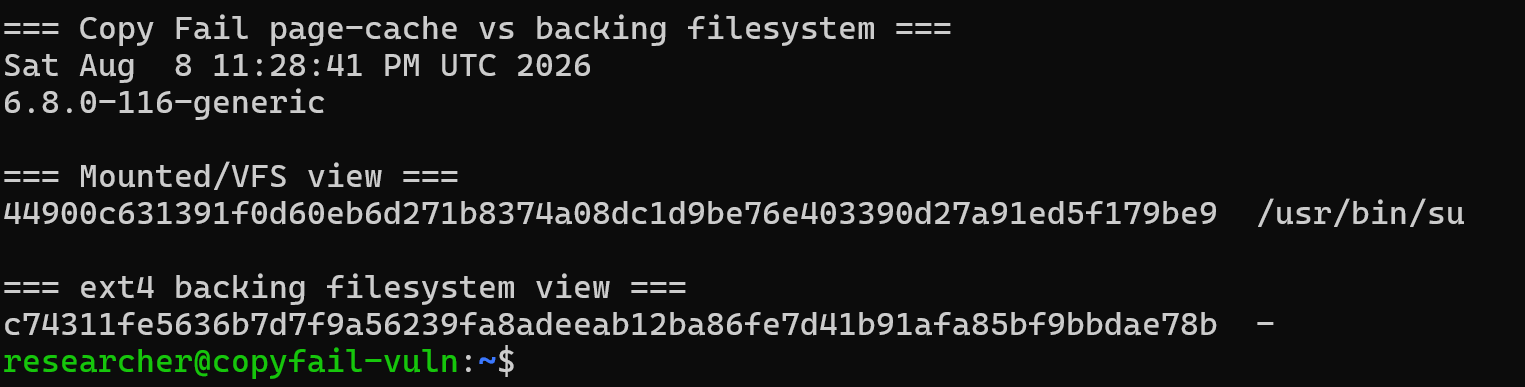
\includegraphics[
        width=\textwidth,
        height=0.31\textheight,
        keepaspectratio
    ]{02-reproduction/screenshots/06-page-cache-vs-backing-filesystem.png}
    \caption{Phase~02 comparison in which the mounted/VFS path returns the
    changed digest while the direct ext4 read returns the original digest.}
    \label{fig:phase02-view-divergence}
\end{figure}

The mounted/VFS read returned the changed digest recorded after exploitation,
while the ext4 read returned the original pre-exploitation digest. The two
access paths therefore produced different byte streams at the comparison point.
That observation is consistent with the published Copy Fail mechanism, where
file-backed cached data can be modified without the same change being written
back to the filesystem \cite{copyfail-research}.

The artifact proves the divergence, not the complete internal explanation. No
kernel instrumentation recorded page objects, dirty flags, scatterlists, or
writeback decisions during this step. The \code{debugfs} command was also a
live point-in-time read, not an offline forensic image. The strongest direct
conclusion is therefore that the mounted and backing-filesystem access paths
returned different content under the tested conditions.

\subsection{Recovery After Reboot}

The final phase recorded the target after rebooting into the same vulnerable
kernel. The screenshot captured at \code{2026-08-08 23:30:53 UTC} shows
\code{6.8.0-116-generic} still active and the mounted path once again returning
the original digest.

\begin{figure}[H]
    \centering
    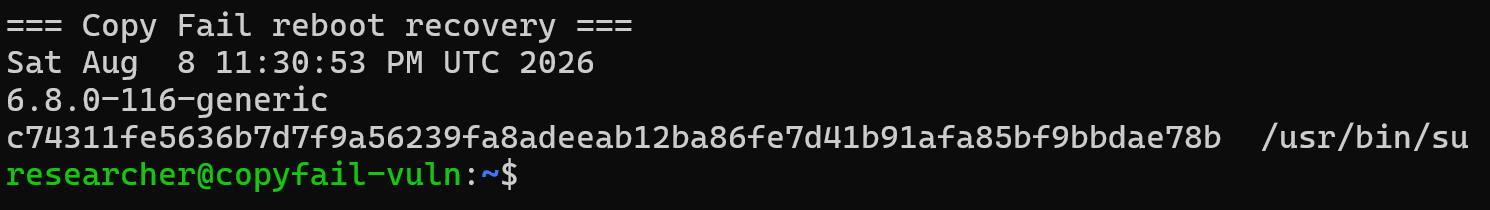
\includegraphics[
        width=\textwidth,
        height=0.22\textheight,
        keepaspectratio
    ]{02-reproduction/screenshots/07-reboot-restores-original-file.png}
    \caption{Post-reboot observation showing the original mounted-view digest
    on the same vulnerable kernel release.}
    \label{fig:phase02-reboot-recovery}
\end{figure}

A later text artifact, timestamped \code{2026-08-08 23:36:42 UTC}, records the
same release and digest and additionally confirms that the target had returned
to its original size, ownership, and SUID mode. These are two post-reboot
observations, not two representations of one simultaneous command.

Because the running release remained \code{6.8.0-116-generic}, the recovery did
not depend on installing a corrected kernel. Under the tested conditions, the
reboot cleared the previously visible mounted-view divergence while the
original backing content remained available.

Recovery is not remediation. The vulnerable kernel and normally loadable module
path were still present, so the prerequisites for another attempt could be
recreated. The recovery captures also do not include a boot identifier, uptime
comparison, or reboot-journal excerpt. They directly establish the recorded
post-reboot state; the reboot event itself is supplied by the documented
experimental sequence.

\subsection{Reproduction Result and Answer to RQ1}

The preserved sequence records a clear before, execution, and recovery path.
VM~271 began on the reconstructed \code{6.8.0-116-generic} runtime with
\code{labuser} at UID~1001 and the selected root-owned SUID target at its
original mounted-view digest. The separate laboratory operator loaded the
required modules. The proof of concept was then launched from the
\code{labuser} prompt, and the resulting shell returned UID~0 and
\code{root}.

\begin{table}[H]
    \centering
    \caption{Claim-to-evidence summary for the controlled reproduction.}
    \label{tab:phase02-findings}
    \small
    \begin{tabularx}{\textwidth}{@{}>{\bfseries\raggedright\arraybackslash}p{0.22\textwidth}>{\raggedright\arraybackslash}p{0.31\textwidth}Y@{}}
        \toprule
        Finding & Direct support & Boundary \\
        \midrule
        Vulnerable runtime active &
        Running release and matching \code{6.8.0-116.116} package records &
        The classification applies to the tested Ubuntu Noble configuration. \\

        Non-root starting identity &
        Item~01 records \code{labuser} at UID~1001 with the ordinary
        \code{users} group &
        The listing records the selected account state, not every possible
        privilege mechanism in the guest. \\

        UID~0 transition &
        Item~03 records \code{id} and \code{whoami} returning UID~0 and
        \code{root} &
        Screenshot-only evidence; the primary group remained GID~1001. \\

        Mounted view changed &
        Items~03 and~05 record the changed target digest &
        A changed digest does not identify the altered bytes or prove on-disk
        replacement. \\

        Read paths diverged &
        Item~06 records different mounted/VFS and ext4-read digests &
        Internal cache and writeback state were not instrumented directly. \\

        Original view recovered &
        Item~07 records the original digest on the same release after the
        declared reboot &
        Recovery does not correct the vulnerable kernel. \\
        \bottomrule
    \end{tabularx}
\end{table}

RQ1 asks whether Copy Fail can be reproduced in the isolated laboratory by an
ordinary, unprivileged local user. For the tested configuration, the answer is
yes. The preserved run starts from the dedicated UID~1001 account and records
the proof-of-concept command producing a UID~0 shell. That identity transition,
not the changed target digest, is the decisive result.

The scope remains deliberately narrow. The preliminary and preserved sequences
show operational repeatability on the same reconstructed VM, but the evidence
does not provide a multi-host trial matrix, a success-rate calculation, or a
statistical timing analysis. The result demonstrates the vulnerability under
the documented conditions; it does not quantify reliability across other
kernels, hardware, workloads, or timing states.

The digest sequence supplies the behavioural context needed for the next stage.
Chapter~6 examines which parts of this activity are observable, which signals
are specific enough to be useful, and how the experiment can move from a
successful reproduction to defensible detection logic.
  \clearpage
  \section{Behavioural Observation and Detection Engineering}
\label{sec:behavioural-detection}

Chapter~5 established the controlled reproduction result and separated the
decisive privilege transition from the accompanying filesystem observations.
The same separation is necessary for detection engineering. A detector may
observe a prerequisite, an action in the exploitation chain, a change to the
target, or the final privileged outcome; these signals occur at different
times and support different conclusions.

The most repeatable host-side effect in the laboratory was the changed content
returned when the selected SUID executable was read through the normal
mounted/VFS path. Its ownership, size, and permission bits remained unchanged,
but its SHA-256 digest differed from the value recorded before exploitation.
This made content integrity a useful detection point even though it did not
identify the proof-of-concept file or explain the internal kernel state that
caused the changed view.

To test that opportunity, a small integrity monitor named MORI was deployed on
VM~271 while it still ran the reconstructed vulnerable kernel. MORI compared a
protected known-good baseline with repeated reads of selected privileged
executables. During a further controlled Copy Fail execution, it reported a
digest mismatch for \code{/usr/bin/su}. The accompanying capture also showed
that the proof of concept obtained a UID~0 shell. The experiment therefore
demonstrated detection of the security-relevant effect, but not prevention of
the exploit.

A separate exact-sample YARA comparison was used to illustrate the difference
between identifying one known proof-of-concept artifact and observing a
host-side consequence. The comparison is deliberately narrow: it evaluates one
rule whose sole condition was the known sample's SHA-256 digest. It is not an
evaluation of YARA as a whole.

This chapter documents the detection model, candidate observables, protected
target baseline, monitor implementation, controlled result, exact-sample
comparison, and operational limitations. It then answers RQ2 and RQ3 within the
evidence actually preserved by the experiment.

\subsection{Detection Model and Evidential Boundary}

The detection question was framed around the privilege boundary rather than
around one exploit filename. The experimentally demonstrated target was
\code{/usr/bin/su}, but the asset being protected was the wider ability to
execute trusted code with elevated credentials. The observed path can be
summarised as:

\begin{lstlisting}
unprivileged local process
    -> vulnerable AF_ALG AEAD path
    -> changed mounted view of a privileged executable
    -> privileged executable launched
    -> UID 0 process
\end{lstlisting}

This representation combines evidence from the vulnerability analysis,
controlled reproduction, and detection phases. It does not mean that every
transition was captured by one telemetry source. In particular, the preserved
detection dataset does not contain a syscall trace, eBPF event stream, or
kernel trace proving the \code{AF\_ALG}, pipe, \code{splice}, and AEAD
operations during the monitored run. Those operations describe the analysed
Copy Fail mechanism and provide candidates for later correlation; the
integrity mismatch and UID~0 outcome are the events directly preserved for
this detection experiment.

The evidence package contains the following principal records:

\begin{table}[H]
    \centering
    \caption{Evidence used in the behavioural detection evaluation.}
    \label{tab:detection-evidence}
    \small
    \begin{tabularx}{\textwidth}{@{}>{\bfseries}p{0.08\textwidth}>{\raggedright\arraybackslash}p{0.31\textwidth}Y@{}}
        \toprule
        ID & Preserved form & Evidential role \\
        \midrule
        00--01 & Text artifacts and screenshots &
        Record the root-owned SUID inventory and which targets were readable
        and executable by \code{labuser}. \\

        02--03 & Baseline and deployment records &
        Preserve the expected target digests and the root-owned operational
        baseline used by the monitor. \\

        04 & Journal excerpt &
        Records MORI's alert for \code{/usr/bin/su}, including the expected
        and observed digests. \\

        07 & Service-status artifact &
        Records the running service, monitored-file count, configured interval,
        and retained alert in the journal. \\

        11--12 & Screenshots &
        Show the alert alongside proof-of-concept execution and, in the latter
        capture, the resulting UID~0 identity confirmation. \\

        YARA & Rule, scan output, and screenshots &
        Compare an exact-hash match for the original sample with a non-match
        after a one-byte, non-executed variation. \\
        \bottomrule
    \end{tabularx}
\end{table}

Screenshot number~08 is intentionally absent from the sequence because the
planned controlled-alert capture was not retained. The numbering is preserved
rather than revised retrospectively. Screenshots~11 and~12 provide useful
concurrent visual context, but the proof-of-concept launch shown in them has no
embedded timestamp. Consequently, the alert timestamp cannot be subtracted
from a verified execution timestamp to produce a measured detection latency.

The public SHA-256 manifests were also rechecked during report preparation.
All listed detector source, service, machine-readable artifacts, rules, and
screenshots used here matched their recorded digests. The two explanatory
\code{README.md} files---the main detection README and the YARA-comparison
README---did not match the digests listed for them. They are therefore treated
as supporting documentation, not as integrity-verified evidence. The
experimental claims below rely on the separately verified artifacts, source,
rule, and captures.

The term \emph{behavioural detection} is used in a host-centric sense in this
chapter: a decision is based on a security-relevant state transition produced
by the tested technique, rather than on the name or exact bytes of the program
that initiated it. MORI observes an effect of the behaviour, not the complete
causal chain. It can report that a protected executable no longer matches its
known-good mounted-view content, but that alert alone cannot attribute the
change specifically to Copy Fail.

\subsection{Observable Stages and Detection Value}

The reproduction exposed several possible observation points. Their defensive
value depends on whether they are direct evidence of exploitation, merely a
precondition, or an outcome that occurs after the security boundary has
already been crossed. \Cref{tab:detection-opportunities} distinguishes these
roles.

\begin{table}[H]
    \centering
    \caption{Candidate observables and their value in the tested attack path.}
    \label{tab:detection-opportunities}
    \small
    \begin{tabularx}{\textwidth}{@{}>{\bfseries\raggedright\arraybackslash}p{0.22\textwidth}>{\raggedright\arraybackslash}p{0.31\textwidth}Y@{}}
        \toprule
        Observable & Experimental status & Detection assessment \\
        \midrule
        Vulnerable kernel and loaded \code{algif\_aead} &
        Both states were recorded before controlled reproduction. &
        Useful exposure context, but neither state proves malicious activity
        and legitimate workloads may require the interface. \\

        AF\_ALG, pipe, \code{splice}, and AEAD sequence &
        Established by the analysed technique, but not directly traced during
        the integrity-monitor run. &
        Potentially useful for selective correlation; not validated as a
        runtime detector in this phase. \\

        Changed privileged-file content through the mounted view &
        Repeatedly observed for \code{/usr/bin/su} and captured by MORI. &
        Strong, sample-independent integrity signal for covered targets, but
        cause-agnostic and detected only after the changed view exists. \\

        Unchanged size, owner, and mode &
        Recorded alongside the changed digest in Chapter~5. &
        Demonstrates that metadata-only monitoring would miss the observed
        content change. \\

        Execution producing UID~0 &
        Directly shown by \code{id} and \code{whoami}. &
        High-confidence confirmation of impact, but too late to be a preventive
        signal in the demonstrated sequence. \\

        Mounted/backing-view divergence and reboot recovery &
        Preserved in the reproduction evidence. &
        Valuable diagnostic context for the transient effect; unsuitable as a
        lightweight continuous detector in the form tested. \\
        \bottomrule
    \end{tabularx}
\end{table}

The module and kernel observations are useful for exposure management. A host
running an affected kernel with \code{algif\_aead} available presents the
tested preconditions, whereas a corrected kernel or an effective module-loading
restriction changes that exposure. These are configuration findings rather
than exploit alerts: the interface may be loaded for legitimate cryptographic
use, and an affected kernel can remain idle indefinitely.

The syscall-level sequence is closer to attacker activity, but individual
operations are not necessarily unique to Copy Fail. A high-fidelity detector
would need to correlate operation type, ordering, process or thread context,
target relationship, and timing while retaining negative controls for benign
AF\_ALG and pipe use. The dataset in this phase does not perform that
correlation. Treating the analysed sequence as already validated telemetry
would therefore overstate the evidence.

The mounted-view digest deviation was the strongest directly tested detection
opportunity. It occurred on the protected side of the interaction, after the
untrusted process had influenced a privileged target but without requiring
knowledge of how the initiating script was named, encoded, or launched. The
same observation appeared in the preliminary investigation, the preserved
reproduction, and the monitored detection test. This supports repeatability on
the same reconstructed guest; it is not a statistical success-rate measurement
across hosts or workloads.

\subsection{Privileged Target Surface and Known-Good Baseline}

The initial target inventory identified 13 root-owned SUID files on the tested
filesystem. From the UID~1001 \code{labuser} account, 12 were recorded as both
readable and executable. The remaining file,
\code{/usr/lib/dbus-1.0/dbus-daemon-launch-helper}, was readable but not
executable in that account context. The experimentally demonstrated target was
\code{/usr/bin/su}; the other reachable SUID files were treated as candidate
privileged targets, not as individually proven Copy Fail targets.

Executables carrying Linux file capabilities were inventoried separately. They
were not added to this first MORI baseline. The distinction matters because the
inventory described a broader privileged-execution surface than the monitor
actually covered. A clean result from MORI therefore means only that the 12
listed SUID paths matched their expected content at the time of a scan.

The baseline stored one SHA-256 digest and one absolute path per monitored
file. For \code{/usr/bin/su}, the expected value was:

\begin{lstlisting}
c74311fe5636b7d7f9a56239fa8adeeab12ba86fe7d41b91afa85bf9bbdae78b
\end{lstlisting}

The complete baseline file had the following digest:

\begin{lstlisting}
c5ebe8afe16326aea860317b153981a43e57f3d462c3e1d03d3d1bbe5d951e74
\end{lstlisting}

Its operational copy was placed at
\code{/etc/copyfail-detector/suid-known-good.tsv}. The preserved deployment
record shows a root-owned directory and a baseline file with mode
\code{-rw-r--r--}, owner \code{root}, group \code{root}, and size
1,016~bytes. An accompanying screenshot records a \code{labuser} modification
attempt being denied. The machine-readable artifact establishes the ownership
and mode; the denied write is screenshot evidence rather than a separately
preserved command transcript.

Root ownership prevents the ordinary test account from silently replacing the
expected values under the recorded permissions, but it is not a complete trust
solution. The baseline must already be correct when generated, legitimate
package updates require controlled regeneration, and an attacker who has
obtained unrestricted root access may be able to alter the baseline, detector,
service definition, or retained logs. MORI's baseline is consequently a
laboratory known-good reference, not an externally attested measurement.

Content hashing was selected because Chapter~5 showed that the target's size,
ownership, and SUID mode remained at their original values while its
mounted-view digest changed. A metadata-only watch would therefore have
reported no relevant difference in that run. Conversely, a digest mismatch
establishes only that the bytes returned by the monitored read differ; it does
not identify the changed offsets, explain their semantics, or prove whether
the persistent backing data was replaced.

\subsection{MORI Integrity Monitor and Service Deployment}

The detector implementation was intentionally small so that its decision could
be traced directly. At start-up, it loads the protected TSV baseline. It then
opens each listed path through the ordinary filesystem interface, reads it in
65,536-byte chunks, calculates SHA-256, and compares the result with the
expected digest. The tested logic can be represented as:

\begin{lstlisting}
baseline = load protected path-to-hash mappings
repeat:
    for each protected path:
        observed = SHA256(read path through normal filesystem view)
        if a new mismatch is observed: emit ALERT
        if a previous mismatch has cleared: emit RECOVERED
    sleep 0.25 seconds
\end{lstlisting}

Reading through the normal filesystem path is central to this experiment. It
places the monitor on the same mounted/VFS view that returned the changed
digest during reproduction. MORI does not inspect the proof-of-concept process
or calculate the proof-of-concept's hash; it repeatedly measures the protected
target content instead.

The set of paths currently in alert state suppresses identical messages on
every scan and permits a later recovery message if a target again matches its
baseline. Missing or unreadable files enter a separate error path. The
implementation does not cryptographically protect its journal output, stop a
changed file from being executed, quarantine a process, or restore target
content. Its decision is a binary equality test against the configured
baseline.

MORI was deployed as a \code{systemd} service with output directed to the
system journal. The service used \code{DynamicUser=yes} and
\code{NoNewPrivileges=yes}, together with a strict read-only system view,
private temporary and device namespaces, kernel and control-group protection,
and \code{RestrictSUIDSGID=yes}. These settings reduce the monitor's own
privilege and writable surface while still allowing it to read the
world-readable protected executables. They do not make the service or journal
tamper-proof against an already privileged attacker.

The status artifact records the service as enabled and active, with the Python
monitor running under PID~3992. Its startup journal entries state:

\begin{lstlisting}
[2026-08-09T15:27:04.563102+00:00] Watching 12 privileged files
[2026-08-09T15:27:04.563133+00:00] Baseline: /etc/copyfail-detector/suid-known-good.tsv
[2026-08-09T15:27:04.563143+00:00] Check interval: 0.25 seconds
\end{lstlisting}

At the later status capture, the service had been active for approximately
1~hour 12~minutes and reported 6.0~MiB of memory, a 6.5~MiB peak, and
52.947~seconds of accumulated CPU time. These values show that the service was
operational for more than an immediate demonstration, but they are a single
status observation rather than a controlled performance benchmark. No disk-I/O
profile, workload comparison, or production-scale target count was measured.

The nominal 0.25-second sleep is likewise not a measured maximum alert delay.
Each scan also requires the time needed to open and hash all listed files, and
the scheduler may add further delay. A sufficiently short-lived mismatch could
occur entirely between observations. Event-driven monitoring or kernel-level
telemetry could reduce that polling limitation, but neither was evaluated by
this detector.

\subsection{Controlled Detection Result}

With the service running on VM~271, the Copy Fail proof of concept was executed
again from the unprivileged \code{labuser} account. Before the monitored
execution, \code{/usr/bin/su} matched the known-good digest. MORI subsequently
emitted the following journal record:

\begin{lstlisting}
[2026-08-09T15:32:31.501808+00:00] ALERT
path=/usr/bin/su
expected=c74311fe5636b7d7f9a56239fa8adeeab12ba86fe7d41b91afa85bf9bbdae78b
observed=44900c631391f0d60eb6d271b8374a08dc1d9be76e403390d27a91ed5f179be9
\end{lstlisting}

The expected value is the original digest recorded before exploitation. The
observed value is the same changed mounted-view digest documented in the
preserved reproduction. This agreement links the detector decision to the
previously characterised host-side effect without requiring the monitor to
recognise the initiating sample.

Screenshots~11 and~12 place the journal alert next to the
\code{labuser} execution terminal. Screenshot~11 shows the proof-of-concept
command returning a \code{\#} prompt; screenshot~12 adds the explicit identity
checks:

\begin{lstlisting}
# id
uid=0(root) gid=1001(labuser) groups=1001(labuser),100(users)
# whoami
root
\end{lstlisting}

As in Chapter~5, the prompt alone is not treated as proof of privilege. The
\code{id} and \code{whoami} output establish the UID~0 outcome. The journal
artifact independently preserves the mismatch event, while the screenshot
provides the concurrent visual relationship between alert and successful
exploitation.

\begin{table}[H]
    \centering
    \caption{Result of the monitored Copy Fail execution.}
    \label{tab:mori-detection-result}
    \small
    \begin{tabularx}{\textwidth}{@{}>{\bfseries\raggedright\arraybackslash}p{0.25\textwidth}>{\raggedright\arraybackslash}p{0.29\textwidth}Y@{}}
        \toprule
        Question & Direct result & Interpretation \\
        \midrule
        Was the protected target changed in the monitored view? &
        MORI reported the documented expected and changed digests for
        \code{/usr/bin/su}. &
        Yes, for the covered target and the tested execution. \\

        Did detection depend on the PoC filename or hash? &
        The detector read only its target baseline and protected paths. &
        No; its decision was independent of the initiating sample's identity. \\

        Was privilege escalation prevented? &
        The adjacent identity checks returned UID~0 and \code{root}. &
        No; the alert was visibility into a successful exploit. \\

        Was detection latency measured? &
        The alert has a journal timestamp, but the visible launch does not. &
        No defensible time-to-alert value can be calculated. \\
        \bottomrule
    \end{tabularx}
\end{table}

No false-positive rate can be derived from this single targeted experiment.
The clean-state captures show that the baseline could be loaded and monitored
without an immediate alert, and the later status record shows no additional
preserved mismatch beyond the \code{/usr/bin/su} event. They do not constitute
a representative benign workload trial. Legitimate package replacement,
administrative maintenance, or any other change to a covered executable would
also produce a digest mismatch until the baseline was reviewed and updated.

\subsection{Exact-Sample YARA Comparison}

The comparison experiment used YARA~4.5.0 on the same
\code{6.8.0-116-generic} environment. Its test rule imported YARA's
\code{hash} module and matched only when the complete scanned file had the
known proof-of-concept SHA-256 digest:

\begin{lstlisting}
d401e7d1c00605749d6c617ace73ab20a762b72e41c2e1590331596e38219a61
\end{lstlisting}

The original 731-byte laboratory sample was scanned without being executed.
At \code{2026-08-09 19:10:18 UTC}, the output recorded:

\begin{lstlisting}
CopyFail_Known_PoC_Exact_Hash /home/labuser/copy_fail_exp.py
yara exit=0
\end{lstlisting}

A private copy was then changed only by appending one trailing newline. Its
size became 732~bytes and its SHA-256 digest became:

\begin{lstlisting}
a567d09b15f6e4440e70c9f2aa8edec8ed59f53301952df05c719aa3911687f9
\end{lstlisting}

The modified file was not executed. At
\code{2026-08-09 19:14:21 UTC}, the exact-hash rule returned no match. The
experiment therefore proves that this particular exact-sample signature
identified the byte-for-byte sample for which it was written and failed after
a trivial byte-level change. It does not prove that the modified file remained
operational, evaded a more general rule, or would evade other static, semantic,
or behavioural detection methods.

This narrow result must not be generalised into a criticism of YARA itself.
YARA rules may use strings, byte patterns, structural properties, modules, and
compound conditions rather than a whole-file digest. The comparison isolates
the limitation of exact-sample identity: it answers whether the scanned bytes
are the one known artifact, not whether the host has experienced the
security-relevant effect associated with Copy Fail.

MORI makes the opposite trade-off. It does not identify the initiating program
at all. A renamed, re-encoded, or otherwise byte-different implementation would
remain outside the detector's concern if it produced no protected-target
change. If it did cause a covered SUID executable to differ from its
known-good mounted-view content for long enough to be scanned, MORI would make
the same comparison regardless of the initiating filename, language, or hash.
That generalisation across initiators is useful, while the loss of causal
specificity remains an operational limitation.

\subsection{Limitations and Answers to RQ2 and RQ3}

The detection result is affirmative but deliberately bounded. The principal
limitations are:

\begin{itemize}
    \item
    only \code{/usr/bin/su} was experimentally demonstrated as a Copy Fail
    target; the other baseline entries are coverage candidates rather than
    individually validated exploit targets;

    \item
    the baseline covered 12 readable and executable root-owned SUID files, not
    file-capability executables, every privileged program, or arbitrary target
    paths;

    \item
    polling can miss an integrity deviation that begins and ends between
    complete scans, and the 0.25-second sleep is not a measured alert latency;

    \item
    a digest mismatch is cause-agnostic and may also result from an authorised
    update, corruption, or another attack technique;

    \item
    the detector alerts after the changed target view exists and did not stop
    the demonstrated UID~0 transition;

    \item
    no syscall or kernel trace directly validated the proposed lower-level
    correlation signals during this monitored run;

    \item
    no representative benign-workload corpus, false-positive rate,
    multi-host trial matrix, or controlled performance benchmark was collected;
    and

    \item
    baseline, detector, and journal trust may be lost after unrestricted root
    compromise unless measurements and alerts are protected or exported
    independently.
\end{itemize}

Within those limits, RQ2 can be answered by separating consistently observed
effects from merely promising telemetry. On the tested VM, the changed
mounted-view content of \code{/usr/bin/su} was the most consistently reproduced
and directly useful system-level detection opportunity. It was visible in the
preliminary investigation, the preserved reproduction, and the monitored
detection run, while size, ownership, and permissions remained unchanged.
The resulting UID~0 identity was a reliable impact confirmation but occurred
too late to support prevention. Vulnerable-kernel and module state supplied
exposure context, whereas the lower-level AF\_ALG and \code{splice}
correlation remained a design candidate rather than a validated detector in
this phase.

RQ3 can also be answered affirmatively for the demonstrated target and
laboratory conditions. MORI detected the exploitation effect without matching
the proof-of-concept filename, programming language, executable hash, or exact
file contents. The one-byte YARA comparison reinforces why that distinction
matters: the exact-hash rule ceased to match after a trivial, non-executed
variation, whereas MORI's decision was anchored to the protected target's
deviation from known-good state.

The answer is not that MORI uniquely identifies Copy Fail. It detects a
security-relevant integrity violation consistent with the reproduced
technique. Attribution would require additional correlation, and timely
prevention requires a control placed earlier in the attack path. The next
chapter therefore moves from observing the changed privileged target to
evaluating a compensating control intended to interrupt the known exploitation
sequence before the privilege boundary is crossed.

  \clearpage
  \section{Custom Compensating Control: MORI}
\label{sec:compensating-control}

Chapter~6 demonstrated that the integrity monitor could recognise a changed
privileged target without identifying the proof-of-concept sample. That result
provided visibility, but it occurred after the protected file view had already
changed and did not prevent the resulting UID~0 transition. RQ4 therefore moves
the defensive decision earlier in the path: can a temporary control interrupt
the known exploitation sequence while the vulnerable kernel is still in use,
and can it avoid removing benign functionality that is not required to be
denied?

The experiment approached this question in two stages. MORI Guard v1 applied a
broad module-loading restriction to \code{algif\_aead}. It stopped the tested
proof of concept on kernel \code{6.8.0-116-generic}, but a benign unprivileged
AF\_ALG AEAD bind failed for the same reason. The result was useful as a safe
baseline: it showed that removing access to the complete interface interrupted
the path, while also making the compatibility cost directly visible.

MORI v2 was then developed as a more selective eBPF and Linux Security Module
(LSM) control. Rather than classifying any one syscall as malicious, it combined
AF\_ALG AEAD activity, a root-owned SUID-file-to-pipe splice, and the associated
privileged-file read in a shared process and thread context. The implementation
was introduced through observation-only checkpoints, negative controls, a
shadow policy, active denial, structured telemetry, adversarial regression
testing, and finally a lifecycle correction in MORI v2.7.

The final control returned \code{EPERM} at the privileged-file permission check
inside the correlated splice operation. The preserved final validation shows
the frozen v2.7 executable denying both the laboratory Python proof of concept
and an independently implemented C proof of concept. In both tests,
\code{labuser} remained UID~1001 and the SHA-256 digest of \code{/usr/bin/su}
remained equal to its known-good value. The result is deliberately narrower
than a claim of universal prevention: MORI v2.7 enforces an experimentally
derived policy for the tested same-process Copy Fail paths and remains a
compensating control rather than a correction to the kernel defect.

This chapter documents the control objective, evidential boundary, broad v1
baseline, incremental v2 development, final enforcement architecture,
lifecycle regression, compatibility controls, adversarial validation, and
remaining limitations. It concludes by answering RQ4 and establishing the
boundary for the vendor comparison in Chapter~8.

\subsection{Control Objective, Success Criteria, and Evidence Boundary}

The compensating-control objective was not merely to make the public Python
script terminate with an error. A useful result had to show where the
interruption occurred, preserve the unprivileged identity, protect the selected
SUID target, and distinguish selective prevention from wholesale interface
removal. The evaluation criteria are summarised in
\cref{tab:mori-success-criteria}.

\begin{table}[H]
    \centering
    \caption{Success criteria used for the custom compensating control.}
    \label{tab:mori-success-criteria}
    \small
    \begin{tabularx}{\textwidth}{@{}>{\bfseries\raggedright\arraybackslash}p{0.24\textwidth}>{\raggedright\arraybackslash}p{0.30\textwidth}Y@{}}
        \toprule
        Criterion & Required observation & Evidential meaning \\
        \midrule
        Known path interrupted &
        The tested proof of concept receives a denial before obtaining a
        privileged shell. &
        Demonstrates prevention for that execution path, not correction of the
        underlying vulnerability. \\

        Privilege boundary preserved &
        Post-test identity remains \code{uid=1001(labuser)}. &
        Excludes an apparent error followed by a successful UID~0 transition. \\

        Privileged target preserved &
        \code{/usr/bin/su} retains the known-good mounted-view SHA-256 digest. &
        Shows that the selected target did not enter the changed state observed
        in Chapter~5. \\

        Benign interface use retained &
        An unprivileged AF\_ALG AEAD control can still reach the tested
        socket, bind, or accept operation. &
        Distinguishes selective enforcement from disabling
        \code{algif\_aead}; it does not prove a complete cryptographic
        round trip. \\

        Individual signals remain permitted &
        AEAD-only, splice-only, and deliberately separated process activity do
        not reach the deny condition. &
        Tests whether the control enforces the correlation rather than treating
        every prerequisite as malicious. \\

        Reproduced defect is regression-tested &
        A test that bypasses an earlier policy version is retained and repeated
        against the corrected candidate. &
        Demonstrates that the final change addresses the observed lifecycle
        failure rather than only changing labels or telemetry. \\
        \bottomrule
    \end{tabularx}
\end{table}

The Phase~04 package contains several evidence classes. MORI Guard v1 is
preserved through machine-readable configuration, blocker source, deployment
state, compatibility output, final retest output, journal events, and
screenshots. MORI v2 preserves complete implementation checkpoints from
v2.2.0 through v2.6.2, screenshots for the earlier v2.1.x work, final v2.7
source and build objects, and the regression and proof-of-concept captures.
This progression is important because the failed designs and compatibility
results are part of the control evaluation rather than discarded development
noise.

The current MORI v2 public manifest contains 108 SHA-256 entries. It includes
the historical checkpoints, the v2.7 source and build set, the current
provenance records, and screenshots~00--57, with the two \code{37a} and
\code{37b} captures retained separately. The older inner
\code{mori-v2/README.md} still reports an 85-object inventory from the earlier
v2.6.2 package. It is therefore used for historical design notes rather than as
the final inventory. The manifest and the current Phase~04 index are the
authoritative package boundaries used in this chapter.

The frozen v2.7 executable is identified by:

\begin{lstlisting}
7fe7b609b90e164f3ae4a9c025363399a8a63bf2a4338db2ecc62cfd2682d039
\end{lstlisting}

That digest is visible before the final Python validation and is repeated in
the frozen artifact manifest and later provenance record. The associated
source files are preserved with the following digests:

\begin{lstlisting}
05e0a387ce084d2aef121351c9af7907f85696307d9f08ccdf6d9191f91a035d
    source/mori_observer.bpf.c
2ee01194b488e757dd4c1062a4123aec8aac5c5cbd74767ebc3a938f886939e6
    source/mori_observer.c
\end{lstlisting}

One chronology boundary must be kept explicit. The final artifact-provenance
record was captured later, when the host reported kernel
\code{6.8.0-137-generic}. It verifies the hashes of the transferred frozen
source and build set; it is not used as evidence of the earlier mitigation-test
kernel. The v1 machine-readable retest and v2.6.2 pre-test capture directly
record \code{6.8.0-116-generic}. The final v2.7 captures identify the tested
binary by hash and show the denial and post-test state, but do not repeat
\code{uname}. The project chronology places those captures in Phase~04 before
the separate vendor-remediation validation. This distinction prevents the
later provenance environment from being substituted for the actual test
sequence.

The evidence supports conclusions about the two tested proof-of-concept
implementations and the stated regression controls. It does not establish a
population-wide prevention rate, production compatibility, or protection
against every possible variation of the vulnerability.

\subsection{MORI Guard v1: Broad Interruption and Compatibility Cost}

MORI Guard v1 used the normal \code{modprobe} configuration mechanism to
redirect requests for \code{algif\_aead} to a root-owned blocker script:

\begin{lstlisting}
install algif_aead /usr/local/sbin/mori-block-algif-aead
\end{lstlisting}

The blocker wrote a structured journal entry, printed the presentation message
to the requesting process when possible, and exited with status~1. The
deployment record shows that \code{modprobe -n -v algif\_aead} resolved to the
custom command, that \code{algif\_aead} was not loaded, and that the existing
MORI integrity monitor remained active. This was an administrative loading
policy, not a change to the vulnerable kernel code.

The final v1 retest was performed by \code{labuser} on
\code{6.8.0-116-generic}. Before the attempt, the account was UID~1001 and
\code{/usr/bin/su} had its expected digest:

\begin{lstlisting}
c74311fe5636b7d7f9a56239fa8adeeab12ba86fe7d41b91afa85bf9bbdae78b
\end{lstlisting}

The proof of concept terminated with \code{FileNotFoundError}, returned exit
status~1, and did not produce a privileged shell. The post-attempt identity
remained \code{labuser}, the target digest was unchanged, and
\code{algif\_aead} remained blocked. The journal recorded the blocker decision,
while the integrity-monitor query returned no event because the protected
target did not change. Within the normal module-loading path exercised by the
test, v1 therefore interrupted the known exploit prerequisite before the
privilege boundary was crossed.

The same mechanism also exposed its compatibility cost. A separate unprivileged
control attempted to bind an AF\_ALG AEAD socket to \code{gcm(aes)}. With v1
active, it failed with \code{FileNotFoundError}, \code{errno=2}, and
\code{No such file or directory}. The failure was expected, but it established
that the control could not distinguish the Copy Fail sequence from a benign
consumer requesting the same kernel interface.

\begin{table}[H]
    \centering
    \caption{Security and compatibility result of MORI Guard v1.}
    \label{tab:mori-v1-result}
    \small
    \begin{tabularx}{\textwidth}{@{}>{\bfseries\raggedright\arraybackslash}p{0.27\textwidth}>{\raggedright\arraybackslash}p{0.25\textwidth}Y@{}}
        \toprule
        Test & Direct result & Interpretation \\
        \midrule
        Python Copy Fail retest &
        PoC failed; UID remained 1001; target hash unchanged. &
        The tested path was interrupted while the vulnerable kernel was
        retained. \\

        Benign \code{gcm(aes)} AEAD bind &
        Failed while the guard was active. &
        The protection was obtained by removing the tested interface from both
        malicious and benign callers. \\

        MORI integrity monitor &
        No target-mismatch event. &
        Consistent with prevention before the monitored target changed; not an
        independent proof of why the PoC failed. \\
        \bottomrule
    \end{tabularx}
\end{table}

The result answers only the first half of RQ4. MORI Guard v1 prevented the
known execution path, but it did so by imposing the exact broad functionality
loss that the second half of the question asks the project to avoid. It
therefore became the compatibility baseline and the motivation for MORI v2.

The scope of the v1 mechanism is also narrower than the phrase ``module
disabled'' may imply. The test validated normal \code{modprobe} resolution
while the module was unloaded. It did not show prevention of direct insertion
by an already privileged administrator, protection when the functionality is
built into the kernel, or resistance to a root user changing the configuration
and blocker script. Those are acceptable boundaries for the temporary
laboratory control, but they prevent it from being described as a kernel fix.

\subsection{From a False Positive to a Selective Policy}

MORI v2 did not begin as an enforcement engine. It was developed by first
observing each candidate signal, then testing whether state could be shared
between hooks, and only later converting the correlation into a denial. The
development sequence is summarised in
\cref{tab:mori-development-progression}.

\begin{table}[H]
    \centering
    \caption{MORI v2 development and the question answered at each checkpoint.}
    \label{tab:mori-development-progression}
    \scriptsize
    \begin{tabularx}{\textwidth}{@{}>{\bfseries}p{0.10\textwidth}>{\raggedright\arraybackslash}p{0.28\textwidth}Y@{}}
        \toprule
        Version & Change & Experimental lesson \\
        \midrule
        v2.1 & Observe non-root reads of root-owned SUID files through
        \code{lsm/file\_permission}. &
        MORI Monitor's legitimate periodic hashing immediately triggered the
        observer; a SUID read alone was too broad. \\

        v2.1.1 & Add a \code{trusted\_tgids} map populated from the monitor's
        service cgroup. &
        The known monitor could be suppressed, while an untrusted SUID read
        remained visible. Cgroup membership alone was still an incomplete
        trust decision. \\

        v2.1.2 & Authenticate the monitor path, file type, owner, permissions,
        SHA-256 digest, cgroup membership, and exact argv entry. &
        Tampering caused trust to be refused. MORI still attached with an empty
        exemption map, making the monitor observable rather than silently
        trusting it. \\

        v2.2 & Observe AF\_ALG \code{aead} bind attempts through
        \code{lsm/socket\_bind}. &
        The hook could see the candidate signal. With v1 disabled, an
        unprivileged \code{gcm(aes)} bind also succeeded, demonstrating that
        observation need not remove the interface. \\

        v2.3 & Record recent AEAD state by TGID and correlate it with a SUID
        read over an experimental ten-second interval. &
        Same-process temporal correlation worked and expired as designed, but
        time proximity did not establish malicious intent. \\

        v2.4 & Observe root-owned SUID-file-to-pipe operations at
        \code{fentry/do\_splice} and share state with the LSM program. &
        Cross-hook state was visible during the same operation; AEAD, splice,
        and SUID-read signals could be combined for one TGID. \\

        v2.5 & Emit \code{WOULD-DENY-}\allowbreak
        \code{AEAD-SPLICE-SUID} while preserving the original LSM return value. &
        The combined path reached the shadow decision, while AEAD-only and
        splice-only controls remained allowed. \\

        v2.6 & Return \code{-EPERM} for the validated correlation. &
        The benign AEAD bind succeeded, but the correlated SUID-to-pipe splice
        was denied with \code{errno=1}. \\

        v2.6.1 & Add a BPF ring buffer containing timestamp, TGID, UID, and
        event type. &
        Userspace received structured deny telemetry, while enforcement
        remained independent of successful event delivery. \\

        v2.6.2 & Add best-effort interactive-terminal notification and extend
        adversarial and target regression testing. &
        The presentation path was separated from the LSM decision. Later
        testing also exposed a same-TGID expiry weakness in the timed state. \\

        v2.7 & Replace the enforcement timer with socket-lifetime AEAD state and
        exact-invocation splice state. &
        The retained 12-second regression was denied, followed by final Python
        and independent C proof-of-concept validation. \\
        \bottomrule
    \end{tabularx}
\end{table}

The first false positive was valuable because it prevented the SUID-read signal
from becoming an unquestioned enforcement rule. The integrity monitor performed
exactly the same low-level action that the prototype observed: it read
root-owned SUID executables. Suppressing it by a hard-coded PID, process name,
or UID would have created a weak exemption. The final userspace loader instead
required a root-owned regular monitor file, no group or world write bit, the
expected SHA-256 digest, an exact command-line argument, and membership in the
dedicated service cgroup before populating the trusted map.

This trust mechanism is an exemption, not the source of the security decision.
If verification fails, MORI emits a warning, attaches its BPF programs, and
leaves the trust map empty. That behaviour favours continued observation over a
silent exemption. It can produce additional monitor noise, but it does not
disable the compensating control simply because the companion monitor could not
be authenticated.

The shadow-policy stage provided a second safety boundary. The combined rule
was allowed to reach a \code{WOULD-DENY} state before any operation was
rejected. AEAD-only and SUID-splice-only negative controls did not reach that
state, whereas the deliberately combined sequence did. Only after this policy
shape was visible did v2.6 change the LSM return value to \code{-EPERM}.
Consequently, active denial was based on a previously observed correlation
rather than introduced at the same time as the first multi-hook test.

\subsection{MORI v2.7 Enforcement Architecture}

The frozen v2.7 candidate consists of a userspace loader and a CO-RE BPF object.
The loader opens and loads the object, authenticates the optional MORI Monitor
exemption, attaches the BPF programs, and polls a ring buffer for deny events.
The kernel-side programs make the enforcement decision. The four principal
state maps are shown in \cref{tab:mori-v27-state}.

\begin{table}[H]
    \centering
    \caption{Kernel-side state used by MORI v2.7.}
    \label{tab:mori-v27-state}
    \small
    \begin{tabularx}{\textwidth}{@{}>{\bfseries\raggedright\arraybackslash}p{0.27\textwidth}>{\raggedright\arraybackslash}p{0.25\textwidth}Y@{}}
        \toprule
        Map & Key and value & Purpose \\
        \midrule
        \code{trusted\_tgids} & TGID $\rightarrow$ one-byte trust flag &
        Suppresses reads from the authenticated MORI integrity-monitor process. \\

        \code{aead\_socket\_state} & BPF socket-local storage $\rightarrow$
        owner TGID, state, and counted flag &
        Associates an observed AF\_ALG AEAD socket with the process that bound
        it and follows the tracked socket until release. \\

        \code{active\_aead\_tgids} & TGID $\rightarrow$ active-socket count &
        Allows enforcement to ask whether the current process owns at least one
        live tracked AEAD socket. \\

        \code{splice\_active\_tids} & TID $\rightarrow$ one-byte active flag &
        Exists only while that exact thread is inside a qualifying
        root-SUID-file-to-pipe \code{do\_splice} invocation. \\

        \code{events} & Ring-buffer records &
        Carries timestamp, TGID, UID, and deny type to userspace on a
        best-effort basis. \\
        \bottomrule
    \end{tabularx}
\end{table}

At \code{lsm/socket\_bind}, MORI first preserves any non-zero decision returned
by a previous LSM program. It then checks for address family~38 (AF\_ALG) and
an algorithm type whose fixed field begins with \code{aead}. The tracked socket
is associated with the current TGID, and the process's active-AEAD count is
incremented. A separate \code{lsm/socket\_accept} program reports an accept only
when the parent socket already carries MORI state. At
\code{fentry/\_\_sock\_release}, the active count is decremented and the
socket-local state is destroyed with the socket.

The implementation therefore makes the lifetime of the tracked socket, rather
than a fixed number of seconds, the relevant AEAD state. The accept event is
useful telemetry, but the frozen source activates and counts the state in the
bind hook. This distinction matters because \code{socket\_bind} observes the
attempt before userspace independently confirms successful completion; it is
retained as a limitation later in this chapter.

At \code{fentry/do\_splice}, the program checks that the caller is non-root,
the input inode is root-owned and carries the owner SUID bit, and the output
inode is a FIFO. If those conditions hold, the current TID is inserted into
\code{splice\_active\_tids}. The corresponding \code{fexit/do\_splice}
program deletes that entry. The state is thus scoped to the exact thread and
the exact invocation instead of remaining available for a grace period after
the operation.

The decision point is \code{lsm/file\_permission}. For a non-root read of a
root-owned SUID file, the program first checks the trusted-monitor exemption.
It then looks for both of the following:

\begin{lstlisting}
active_aead_tgids[current TGID] > 0
splice_active_tids[current TID] == 1
\end{lstlisting}

When both are present, MORI submits a ring-buffer event if space is available,
writes a trace message, and returns \code{-1}, corresponding to
\code{-EPERM}. If either condition is absent, the previous LSM result is
preserved. The policy interrupts the file read used inside the qualifying
splice; it does not wait for the later page-cache change or privileged-program
execution observed in Chapters~5 and~6.

The tested policy boundary is summarised in
\cref{tab:mori-v27-policy-boundary}.

\begin{table}[H]
    \centering
    \caption{Decision boundary implemented by the frozen MORI v2.7 source.}
    \label{tab:mori-v27-policy-boundary}
    \small
    \begin{tabularx}{\textwidth}{@{}>{\raggedright\arraybackslash}p{0.43\textwidth}>{\bfseries\raggedright\arraybackslash}p{0.16\textwidth}Y@{}}
        \toprule
        Observed condition & Decision & Reason \\
        \midrule
        Ordinary socket activity or non-AEAD AF\_ALG activity & Allowed &
        No tracked AEAD socket is created by the tested predicate. \\

        AF\_ALG AEAD activity without a qualifying splice & Allowed &
        The splice-invocation state is absent. \\

        Root-owned SUID file spliced to a pipe without same-process active AEAD
        state & Allowed &
        The active-AEAD count is absent or zero. \\

        AEAD activity in process A and SUID-to-pipe splice in process B &
        Allowed &
        AEAD state is isolated by TGID rather than correlated across processes. \\

        Live tracked AEAD socket in the same TGID, with the current TID inside
        the qualifying splice and reading the SUID input & Denied with EPERM &
        Both enforcement states are present at the protected read. \\

        Authenticated MORI Monitor read & Allowed &
        The trusted TGID exemption is evaluated before correlation. \\

        Root caller & Allowed by this policy &
        The control is designed to interrupt the pre-escalation non-root path,
        not constrain an already privileged process. \\
        \bottomrule
    \end{tabularx}
\end{table}

Structured telemetry is deliberately downstream of the decision. If the ring
buffer is full or the userspace process is unavailable, reservation can fail,
but the LSM program still returns \code{EPERM}. When userspace does receive the
event, it prints the TGID and UID and optionally searches
\code{/proc/<tgid>/fd/} for descriptors~2, 1, and~0. Each candidate is opened
independently and checked with \code{isatty()} before the cosmetic MORI message
is written. Failure to find or write a terminal changes neither the kernel
decision nor the denied process's return value.

\subsection{Regression-Driven Lifecycle Correction}

MORI v2.6.2 used timestamps keyed by TGID. AEAD state and splice state were
considered relevant only within an experimental ten-second interval. That
design passed the original short positive tests, but later adversarial testing
kept the same process and AEAD socket alive, waited 12~seconds, and then spliced
\code{/usr/bin/fusermount3} into a pipe. The trace showed the expected AEAD and
splice observations, yet userspace reported:

\begin{lstlisting}
same-TGID expiry test: tgid=8358
AEAD armed; waiting 12 seconds...
splice allowed after expiry: 32 bytes
\end{lstlisting}

This was a reproduced bypass of the selected v2.6.2 policy. It was not a
separate demonstration of UID~0 or target corruption, but it proved that the
timer could expire while the relevant socket and process remained active. The
control had therefore encoded elapsed time rather than the lifecycle of the
operation it was trying to constrain.

The first v2.7 lifecycle candidate was also retained rather than treated as a
successful fix. It recorded an \code{AEAD-CANDIDATE} and the later splice, but
the active state did not reach the permission decision; after the same
12-second delay, 32~bytes were still spliced. This intermediate failure showed
that merely adding socket-local state was insufficient unless the state
transition consulted by enforcement matched the AF\_ALG socket behaviour in
the test.

The frozen v2.7 source corrected the design in two ways:

\begin{enumerate}
    \item
    the AEAD association is counted for the lifetime of the tracked bound
    socket and released during socket teardown, with elapsed time retained only
    for event timestamps; and

    \item
    the splice flag is keyed by TID and exists only between
    \code{fentry/do\_splice} and \code{fexit/do\_splice} for that exact
    invocation.
\end{enumerate}

The retained regression again kept the AEAD operation socket open and waited
12~seconds before attempting the same SUID-to-pipe splice. This time the trace
contained \code{AEAD-ACTIVE}, \code{SPLICE-ARM}, and
\code{DENY-AEAD-SPLICE-SUID}; userspace received:

\begin{lstlisting}
v2.7 lifecycle regression: tgid=9531
AEAD socket active; waiting 12 seconds...
splice blocked: errno=1 (Operation not permitted)
\end{lstlisting}

The result addresses the specific expiry defect because the same delayed
sequence changed from allowed to denied after lifecycle state replaced the
timer. It does not prove that every socket-transfer, fork, exec, concurrency,
or teardown case is correct. Those cases were outside the preserved regression
matrix.

Cross-TGID isolation remained intentional. A v2.6.2 control held AEAD state in
one process while another process spliced the SUID target; the second process
successfully moved 32~bytes. The final v2.7 source retains process ownership for
AEAD state, so it does not create a host-wide correlation merely because two
unrelated processes perform the individual operations. This reduces broad
coupling between benign workloads, while also defining an evasion boundary if
an untested exploit implementation can distribute the required sequence across
processes.

\subsection{Adversarial Validation of the Frozen Candidate}

The final validation used the v2.7 executable whose digest begins
\code{7fe7b609}. The capture shows the userspace loader verifying the MORI
Monitor file, trusting TGID~702, attaching the enforcement engine, and
announcing that selective policy and structured telemetry were active. The
same executable remained running for the final Python and independent C tests;
the Phase~04 index records that it was not rebuilt between them.

\subsubsection{Python proof of concept}

The actual Python execution was performed after switching into the unprivileged
\code{labuser} account. A preliminary command in the same capture used an
incorrect home-directory expansion and failed before the test; it is not
counted as the security result. During the subsequent execution from
\code{/home/labuser}, the BPF trace recorded the following lifecycle for the
same TGID and TID:

\begin{lstlisting}
AEAD-ACTIVE
AEAD-ACCEPT-OBSERVED
SPLICE-ARM
DENY-AEAD-SPLICE-SUID
SPLICE-DISARM ret=-1
AEAD-RELEASE
\end{lstlisting}

The proof of concept was stopped by the LSM decision:

\begin{lstlisting}
PermissionError: [Errno 1] Operation not permitted
\end{lstlisting}

MORI userspace received the structured deny event for UID~1001 and delivered
the optional terminal notification. The security-relevant result is the LSM
\code{EPERM}; the message is presentation only.

Post-test validation recorded \code{labuser} as UID~1001 and returned the
known-good digest for \code{/usr/bin/su}:

\begin{lstlisting}
c74311fe5636b7d7f9a56239fa8adeeab12ba86fe7d41b91afa85bf9bbdae78b
\end{lstlisting}

The target therefore did not enter the changed mounted-view state used by MORI
Monitor in Chapter~6, and the test did not produce the UID~0 outcome seen during
the unmitigated reproduction.

\subsubsection{Independent C proof of concept}

The second validation used a separately implemented C proof of concept. Its
preserved provenance records the following identifiers:

\begin{lstlisting}
commit  ba3f503b1497350a2df3a89fab0427b4f868fe59
source  e1dec1348c0d43ab47d8f992d9a0336216fd37ff83e6fa1d9e39a80890fbd165
binary  3b2605dc5e820f40645f682385194469f9189cbb65ee99153b52aedf45be5706
\end{lstlisting}

Some provenance commands at the top of the combined validation capture were
run from the wrong directory and failed. They are not used for these values;
the separate provenance capture records the successful commit and hash output.

The C test reported that its first attempted write failed. The trace again
showed \code{AEAD-ACTIVE}, an observed accept, \code{SPLICE-ARM}, the v2.7
deny event, splice disarm with return value~$-1$, and AEAD release. After the
test, the account remained UID~1001 and \code{/usr/bin/su} retained the same
known-good digest. No privileged shell was observed.

\begin{table}[H]
    \centering
    \caption{Final adversarial results for the frozen MORI v2.7 candidate.}
    \label{tab:mori-v27-adversarial-results}
    \small
    \begin{tabularx}{\textwidth}{@{}>{\bfseries\raggedright\arraybackslash}p{0.20\textwidth}>{\raggedright\arraybackslash}p{0.24\textwidth}>{\raggedright\arraybackslash}p{0.23\textwidth}Y@{}}
        \toprule
        Test & Denial observation & Post-test identity and target & Conclusion \\
        \midrule
        Python PoC &
        Correlated splice returned \code{EPERM}; matching kernel and ring-buffer
        events were visible. &
        UID~1001; \code{/usr/bin/su} hash matched baseline. &
        Known Python path prevented. \\

        Independent C PoC &
        First attempted write failed after the matching v2.7 deny lifecycle. &
        UID~1001; \code{/usr/bin/su} hash matched baseline. &
        Second implementation path prevented. \\
        \bottomrule
    \end{tabularx}
\end{table}

The two implementations reduce dependence on one script's error handling or
layout. They do not make the sample size large and do not establish resistance
to all Copy Fail variants. The strongest supported statement is that the same
frozen v2.7 candidate interrupted both tested same-process paths before the
documented target change and privilege transition.

\subsection{Compatibility and Negative Controls}

Compatibility was evaluated incrementally rather than inferred from the final
denial alone. The most important contrast is between v1 and v2: v1 made even a
benign \code{gcm(aes)} bind unavailable, whereas the v2 series kept
\code{algif\_aead} loaded and allowed the tested benign AEAD operation before
selectively denying the correlated SUID splice.

The preserved controls are summarised in
\cref{tab:mori-compatibility-controls}. Version labels are retained because not
every earlier negative control was repeated in a separate capture against the
frozen v2.7 binary.

\begin{table}[H]
    \centering
    \caption{Compatibility, negative, and regression controls across MORI development.}
    \label{tab:mori-compatibility-controls}
    \scriptsize
    \begin{tabularx}{\textwidth}{@{}>{\bfseries}p{0.12\textwidth}>{\raggedright\arraybackslash}p{0.32\textwidth}>{\raggedright\arraybackslash}p{0.20\textwidth}Y@{}}
        \toprule
        Version & Control & Direct result & Meaning \\
        \midrule
        v1 & Unprivileged \code{gcm(aes)} AF\_ALG AEAD bind & Failed &
        Broad interface removal imposed a demonstrated compatibility cost. \\

        v2.2 & Same benign AEAD bind with v1 disabled & Succeeded and was
        observed &
        Observation did not itself require disabling AEAD. \\

        v2.5 & AEAD-only and SUID-splice-only shadow tests & Allowed; no
        \code{WOULD-DENY} &
        Neither individual signal was sufficient for the selected policy. \\

        v2.6 & Combined enforcement test & AEAD bind succeeded; correlated
        splice returned \code{EPERM} &
        The denial boundary could be placed after benign interface access. \\

        v2.6.2 & Cross-TGID AEAD and splice & Splice allowed &
        State was isolated by process rather than combined host-wide. \\

        v2.6.2 & SUID-target sweep & Attempts were denied; ten recorded target
        hashes remained unchanged &
        The predicate was not hard-coded only to \code{/usr/bin/su}; this was a
        v2.6.2 regression, not a universal target claim. \\

        v2.6.2 & Same-TGID operation after 12-second delay & Splice allowed &
        Reproduced a timer-based policy bypass. \\

        v2.7 & Same delayed lifecycle regression & Splice denied with
        \code{EPERM} &
        Socket-lifetime state addressed the reproduced expiry defect. \\

        v2.7 & Python and independent C PoCs & Both denied &
        The frozen candidate interrupted both final implementation paths. \\
        \bottomrule
    \end{tabularx}
\end{table}

The ten-target post-sweep capture lists \code{chfn}, \code{chsh},
\code{fusermount3}, \code{gpasswd}, \code{mount}, \code{newgrp},
\code{passwd}, \code{su}, \code{sudo}, and \code{umount} as unchanged. The
test demonstrates that the root-owner and SUID predicates could operate across
multiple recorded targets and that those targets retained their baseline
digests after the denied operations. It does not show that each program is an
independently exploitable Copy Fail target.

The benign AEAD evidence must also be interpreted narrowly. The v2.2 control
established a successful unprivileged \code{gcm(aes)} bind, and later controls
recorded bind and accept availability where stated. The dataset does not
preserve a complete encryption/decryption round trip or a representative
application workload. ``Benign functionality preserved'' therefore means that
MORI v2 did not remove the tested AF\_ALG AEAD interface operations and left
the isolated negative controls available. It does not mean that every legitimate
AEAD consumer was tested or that the control has zero compatibility impact.

\subsection{Operational and Security Limitations}

MORI v2.7 is an experimental, privileged, host-local compensating control. Its
result is useful because it is selective relative to v1, but several boundaries
prevent it from being treated as a general Linux exploit-prevention system.

\begin{itemize}
    \item
    \textbf{The vulnerable code remains present.} MORI denies an observed
    combination before the tested exploit reaches its target; it does not
    correct the \code{algif\_aead} implementation. Detaching the BPF programs,
    changing the loader, or booting without the required policy restores the
    underlying exposure.

    \item
    \textbf{The policy recognises behaviour, not intent.} AF\_ALG AEAD use and
    SUID-to-pipe splice activity can each be legitimate. A benign program that
    reproduces the complete same-process and same-thread combination may receive
    \code{EPERM}.

    \item
    \textbf{Process isolation creates an evasion boundary.} AEAD state is
    associated with an owner TGID. Cross-TGID activity is intentionally allowed.
    An untested implementation able to divide the required operations between
    processes, transfer descriptors, or otherwise change ownership semantics
    may fall outside the policy.

    \item
    \textbf{Bind observation precedes independent success confirmation.} The
    frozen source increments active state in \code{lsm/socket\_bind}. A later
    accept is separately observed, but enforcement consults the count created
    at bind. A failed bind whose socket remains open can therefore create
    conservative state until release. This was not evaluated across a corpus of
    failing benign applications.

    \item
    \textbf{Thread and lifecycle coverage is tested, not exhaustive.} TID-scoped
    splice state improves the precision of the permission decision, but fork,
    exec, descriptor passing, multithreaded races, abnormal teardown, and PID or
    TGID reuse were not subjected to a complete regression matrix.

    \item
    \textbf{Map-update failures allow the operation.} Source review shows that
    failure to allocate or update the active-AEAD or splice state is logged and
    the original operation is preserved. This avoids turning internal pressure
    into an uncontrolled system-wide denial, but it is fail-open for the
    compensating policy.

    \item
    \textbf{Monitor trust is local and start-up based.} The loader authenticates
    the monitor file and current service-cgroup processes before inserting TGIDs.
    The preserved source does not demonstrate continuous revalidation or removal
    of a trusted entry when the process lifecycle changes.

    \item
    \textbf{Telemetry is best-effort.} Ring-buffer exhaustion or userspace
    failure does not weaken a decision whose state was successfully created, but
    it can remove structured context and the optional TTY notification. Kernel
    trace output is also diagnostic rather than an independently protected audit
    trail.

    \item
    \textbf{Deployment depends on kernel facilities.} The tested design requires
    BPF LSM attachment, BTF/CO-RE information, the selected LSM and fentry hooks,
    and sufficient administrative privilege. The frozen provenance records
    clang~18.1.3 and libbpf~1.3.0, but no cross-distribution, cross-architecture,
    or production-kernel portability matrix was collected.

    \item
    \textbf{Performance and false-positive rates were not measured.} The
    experiment contains targeted positive and negative controls, not a sustained
    representative workload, controlled overhead benchmark, or statistical
    false-positive study.

    \item
    \textbf{The final evidence remains bounded.} Two proof-of-concept
    implementations, one principal target, an alternate target, and the stated
    regression suite improve confidence in the selected path. They do not prove
    protection against every algorithm, target, sequencing variation, or future
    exploitation technique.
\end{itemize}

The attacker-facing message deserves no separate security credit. It is useful
for demonstrating that the structured event reached userspace, but it also
reveals that a policy intervened and depends on access to an interactive
terminal. Removing it would not change the LSM result; losing it does not mean
the denial failed.

These limitations do not invalidate the experiment. They define what the
control achieved: a narrower temporary denial than complete interface removal,
with a documented policy, reproducible negative controls, a retained bypass,
and a regression-tested correction. They also explain why a vendor kernel fix
remains the preferred remediation.

\subsection{Answer to RQ4 and Transition to Vendor Comparison}

RQ4 asks whether a defensive control can interrupt the known exploitation path
before the kernel is patched and whether it can do so without unnecessarily
removing benign functionality. The experiments produce two different answers.

MORI Guard v1 answers the prevention part affirmatively but the compatibility
part negatively. On the vulnerable \code{6.8.0-116-generic} runtime, it kept
\code{algif\_aead} unavailable through the tested \code{modprobe} path, caused
the Python PoC to fail, preserved UID~1001, and kept \code{/usr/bin/su}
unchanged. The same restriction also caused the benign \code{gcm(aes)} bind to
fail. It interrupted the exploit by removing the complete tested interface.

The final MORI v2.7 result supports an affirmative but bounded answer to both
parts. The frozen candidate left AF\_ALG AEAD available in the exercised
controls and allowed individual or cross-process signals that did not satisfy
the policy. It denied the correlated SUID-to-pipe operation with \code{EPERM}
for both the Python and independent C proof-of-concept paths. After each test,
\code{labuser} remained UID~1001 and the selected privileged target retained
its known-good digest. The retained 12-second regression also shows that the
final lifecycle design corrected a specific bypass present in v2.6.2.

The qualifier is essential. MORI v2.7 preserves more benign functionality than
v1 because it does not remove the AEAD interface and does not deny every
individual prerequisite. It does not establish that all benign applications
remain unaffected, and process separation, state-allocation failure, lifecycle
edge cases, or a variant outside the selected correlation may evade it. The
appropriate conclusion is therefore:

\begin{lstlisting}
For the tested same-process Copy Fail paths in the Phase 04 laboratory,
MORI v2.7 interrupted exploitation before privilege escalation while
preserving the benign interface operations and negative controls that
were exercised. It is a selective compensating control, not a patch and
not proof of universal prevention.
\end{lstlisting}

This chapter deliberately stops short of answering RQ5. MORI Guard v1 and
Canonical's temporary mitigation both restrict \code{algif\_aead}, whereas
MORI v2.7 attempts a narrower behavioural decision inside the active interface.
Chapter~8 compares those approaches directly: what each blocks, what each
preserves, the trust and deployment assumptions each introduces, and why the
custom result does not replace vendor-supported remediation.
  \clearpage
  \section{Vendor Mitigation and Comparative Evaluation}
\label{sec:vendor-mitigation}

Chapter~7 showed that a custom compensating control could interrupt the tested
Copy Fail paths while the vulnerable kernel remained active. It also showed why
the word \emph{custom} matters. MORI Guard v1 achieved broad prevention by
removing access to \code{algif\_aead}, whereas MORI v2.7 preserved the tested
interface operations by enforcing a narrower behavioural correlation. RQ5 now
places those results beside Canonical's temporary response:

\begin{quote}
\textbf{RQ5 -- Vendor Comparison.} How does the custom compensating control
compare with Canonical's temporary mitigation, which prevents
\code{algif\_aead} from being loaded?
\end{quote}

The comparison is not a contest in which the most selective mechanism wins by
definition. A broad vendor mitigation may be preferable because it is simple,
packaged, supportable, and intentionally conservative. A selective research
control may preserve more functionality, but only within the behaviour and
environment that its policy actually recognises. The evaluation must therefore
consider prevention scope, compatibility, operational complexity, evidential
strength, telemetry, and the route back to an ordinary patched system.

The resulting answer is deliberately asymmetric. MORI Guard v1 belongs to the
same policy class as Canonical's temporary mitigation and offers no compatibility
advantage over it. MORI v2.7 demonstrates that the tested exploitation path can
be interrupted without removing the tested AF\_ALG AEAD operations, but it does
so with narrower assurance and substantially greater implementation and
deployment complexity. Neither custom control corrects the kernel defect, and
neither should displace the vendor kernel update as the final remediation.

\subsection{Comparison Objective and Evidence Boundary}

The comparison uses three evidence classes. First, Canonical's security notice
and technical guidance define the purpose, package version, deployment action,
compatibility warning, and intended lifetime of the temporary mitigation
\cite{ubuntu-copyfail-fixes,ubuntu-copyfail-cve}. Second, Phase~01 records the
policy as it appeared on the preserved Ubuntu reference guest. Third, Phase~04
contains the direct vulnerable-kernel experiments for MORI Guard v1 and MORI
v2.7.

These classes answer different questions. Vendor documentation states what the
distribution intended to deploy. Phase~01 shows the effective module-resolution
rule on the reference system. Phase~04 shows what happened when the laboratory's
custom controls were exercised on \code{6.8.0-116-generic}. None of these alone
creates a perfectly matched head-to-head trial.

In particular, the Canonical \code{kmod} policy was captured on a reference
guest whose running \code{6.8.0-137-generic} kernel was already corrected. A
Copy Fail execution on that combined state would have had two independent
reasons to fail: the ordinary module-loading path was restricted and the kernel
contained the vendor correction. The project therefore did not use that guest
as a causal exploit test for the temporary mitigation. By contrast, MORI Guard
v1 was directly tested on \code{6.8.0-116-generic}, and the Phase~04 chronology
places the final MORI v2.7 validation before vendor remediation. The final v2.7
captures identify the frozen binary and result but do not repeat \code{uname};
their kernel attribution is therefore sequence-based rather than a repeated
runtime capture.

The comparison criteria are summarised in \cref{tab:vendor-comparison-criteria}.

\begin{table}[H]
    \centering
    \caption{Criteria used for the vendor-mitigation comparison.}
    \label{tab:vendor-comparison-criteria}
    \small
    \begin{tabularx}{\textwidth}{@{}>{\bfseries\raggedright\arraybackslash}p{0.23\textwidth}>{\raggedright\arraybackslash}p{0.32\textwidth}Y@{}}
        \toprule
        Criterion & Question & Boundary \\
        \midrule
        Prevention scope &
        Which prerequisite or behaviour is denied? &
        Broader coverage can reduce evasion space while increasing collateral
        impact. \\

        Compatibility &
        Which benign operations remain available? &
        Only operations actually exercised by the preserved controls are
        credited. \\

        Evidential strength &
        Was the result directly tested on the vulnerable runtime or inferred
        from the mechanism and vendor record? &
        Mechanism-based confidence is kept separate from experimental causality. \\

        Operational burden &
        What must be installed, loaded, maintained, and recovered? &
        Laboratory feasibility does not establish production suitability. \\

        Observability &
        What security-relevant context accompanies a denial? &
        Telemetry is useful, but it does not compensate for an incomplete
        prevention boundary. \\

        Remediation lifecycle &
        How is the control retired after a fixed kernel is active? &
        A temporary control should have a clear and supportable exit path. \\
        \bottomrule
    \end{tabularx}
\end{table}

This boundary prevents two overstatements. The chapter does not claim that the
Canonical rule was independently proven as the sole cause of exploit failure
on the vulnerable laboratory kernel. It also does not treat the successful
MORI v2.7 controls as proof that every legitimate AF\_ALG workload remains
compatible or that every Copy Fail implementation is recognised.

\subsection{Canonical's Temporary \texttt{kmod} Mitigation}

Canonical published \code{kmod} updates on 30 April 2026 to block loading of
the affected \code{algif\_aead} module until kernel updates became available.
For Ubuntu 24.04 LTS Noble, the mitigation-bearing package version was
\code{31+20240202-2ubuntu7.2} \cite{ubuntu-copyfail-fixes}. Canonical's manual
equivalent writes the following \code{modprobe} install rule:

\begin{lstlisting}
install algif_aead /bin/false
\end{lstlisting}

An install rule substitutes the specified command for the module insertion
performed through normal \code{modprobe} resolution. Requests may still resolve
the dependency path, but the \code{algif\_aead} insertion itself is replaced by
\code{/bin/false}. The mechanism does not inspect the caller, target file,
splice activity, or intended cryptographic operation. It removes the affected
module from that ordinary loading path for every caller.

The rule is preventive only when the module is not already active. Canonical's
guidance therefore instructs administrators to unload \code{algif\_aead} when
possible or reboot when the module is in use. The same guidance warns that
applications may fall back to userspace cryptography, but that the fallback is
not guaranteed and already running applications may be affected
\cite{ubuntu-copyfail-fixes}. This is not an incidental weakness in the
mitigation; it is the explicit trade-off of removing an attack surface before a
corrected kernel can be deployed.

\subsubsection{Observed reference-system policy}

Phase~01 captured the following state on the Ubuntu reference guest:

\begin{lstlisting}
kmod                                  31+20240202-2ubuntu7.2
linux-image-6.8.0-137-generic         6.8.0-137.137

/etc/modprobe.d/disable-algif_aead.conf:
install algif_aead /bin/false
\end{lstlisting}

The corresponding dry run resolved to insertion of the dependency
\code{af\_alg} followed by \code{install /bin/false}; the module-state capture
contained no loaded \code{algif\_aead} entry. The installed kernel configuration
also recorded \code{CONFIG\_CRYPTO\_USER\_API\_AEAD=m}, so the affected
interface was a loadable module on this system rather than compiled directly
into the kernel.

This evidence confirms the effective policy and its suitability for the
captured Ubuntu configuration. It does not establish resistance to an
administrator deliberately changing the configuration, nor does it test every
low-level way privileged code might be introduced. Those cases fall outside the
unprivileged local-attacker model used by the project. More importantly for RQ5,
the capture proves policy presence and resolution behaviour, not a standalone
vulnerable-kernel exploit result.

\subsubsection{Intended lifetime}

Canonical described the \code{kmod} change as temporary and recommended
upgrading to a fixed kernel and rebooting. Its published Noble generic-kernel
boundary identifies \code{6.8.0-117.117} as fixed
\cite{ubuntu-copyfail-cve}. Once a corrected kernel is active, the loading rule
is no longer required and may itself become an unnecessary compatibility
restriction. Canonical's guidance consequently includes a documented route for
disabling the mitigation after the kernel update
\cite{ubuntu-copyfail-fixes}.

This lifecycle is a significant operational advantage. The mitigation is
distributed through the ordinary package channel, tied to a vendor advisory,
and explicitly superseded by a kernel update. Its purpose is emergency risk
reduction, not permanent replacement of AF\_ALG AEAD.

\subsection{Relationship to MORI Guard v1}

MORI Guard v1 used the same system mechanism but redirected the module request
to a laboratory blocker:

\begin{lstlisting}
install algif_aead /usr/local/sbin/mori-block-algif-aead
\end{lstlisting}

The blocker returned failure, wrote a structured journal event, and attempted
to present the MORI message to the requesting process. On
\code{6.8.0-116-generic}, the Python proof of concept failed, \code{labuser}
remained UID~1001, and \code{/usr/bin/su} retained its known-good digest. A
separate unprivileged \code{gcm(aes)} bind also failed while the guard was
active.

At the policy level, Canonical's mitigation and MORI Guard v1 are therefore
equivalent in breadth for the tested Ubuntu module configuration: both replace
ordinary loading of \code{algif\_aead} with a failing command. The custom script
changes the presentation and evidence available to the laboratory, not the
fundamental compatibility boundary. Both deny malicious and benign callers
before either can use the module.

There are nevertheless operational differences:

\begin{itemize}
    \item Canonical's rule arrives in a signed distribution package and is
    documented as part of the vendor response. MORI Guard v1 is a locally
    authored configuration and script whose review, deployment, and removal
    remain the operator's responsibility.

    \item MORI Guard v1 emits a dedicated journal record and a recognisable
    presentation message. Canonical's rule provides a generic command failure;
    the vendor guidance does not define equivalent structured Copy Fail deny
    telemetry.

    \item MORI Guard v1 was directly exercised against the vulnerable kernel in
    the laboratory. The captured Canonical rule was validated on the already
    patched reference guest and is supported by the vendor's stated mechanism,
    not by an otherwise identical laboratory exploit trial.

    \item Both depend on the module being absent when enforcement begins. A
    loading rule does not retroactively detach an active module, so operational
    validation must include module state or a reboot.
\end{itemize}

For an ordinary Ubuntu deployment awaiting a kernel update, MORI Guard v1 does
not offer a security or compatibility reason to replace the vendor package. Its
additional value is limited to the research environment, where the custom
blocker made the control decision visible and provided a locally controlled
comparison baseline.

\subsection{Relationship to MORI v2.7}

MORI v2.7 begins from the opposite compatibility decision. It leaves
\code{algif\_aead} available and denies only when the tested same-process
correlation reaches the protected privileged-file read. The frozen candidate
combines live AEAD socket state, exact-invocation SUID-file-to-pipe splice
state, a non-root read of the selected class of root-owned SUID file, and an
authenticated monitor exemption.

This design produced two useful differences from the module-level controls:

\begin{enumerate}
    \item The unprivileged \code{gcm(aes)} socket, bind, and later recorded
    accept operations remained available where tested. AEAD-only and
    splice-only negative controls did not reach the deny decision.

    \item A matched decision produced \code{EPERM} together with kernel trace
    output and a structured ring-buffer event containing the TGID, UID,
    timestamp, and deny type. The telemetry exposed why the policy intervened
    rather than only reporting that module insertion failed.
\end{enumerate}

The selectivity is real within the preserved test matrix, but it changes the
assurance model. Canonical's mitigation prevents the complete module-dependent
path through ordinary module resolution. MORI v2.7 must correctly observe and
correlate the exploit's behaviour. A variant that separates work across
processes, changes ownership semantics, avoids a monitored hook, or falls
outside the selected SUID-to-pipe sequence may evade the policy. Conversely, a
legitimate program that reproduces the full correlation may receive
\code{EPERM}.

MORI v2.7 also introduces dependencies that the \code{kmod} rule does not have:
BPF LSM support, BTF and CO-RE information, the selected LSM and tracing hooks,
a privileged userspace loader, map allocation, state lifecycle correctness,
and optional monitor authentication. The Phase~04 source review further shows
that state-map update failures preserve the original operation. That choice
avoids turning allocation pressure into an uncontrolled denial of service, but
it is fail-open for the compensating policy.

The appropriate conclusion is therefore not that selective correlation is
strictly better than broad removal. MORI v2.7 trades some breadth and
operational simplicity for retained tested functionality and richer decision
context. Whether that exchange is acceptable depends on the system's workload,
kernel facilities, risk tolerance, and the length of time for which the
vulnerable kernel must remain in service.

\subsection{Security Coverage and Failure Modes}

The three controls can be ordered by where they intervene, but not by a single
universal measure of strength. \Cref{tab:vendor-security-comparison} separates
the supported security claims.

\begin{table}[H]
    \centering
    \caption{Security boundary of the temporary controls.}
    \label{tab:vendor-security-comparison}
    \scriptsize
    \begin{tabularx}{\textwidth}{@{}>{\bfseries\raggedright\arraybackslash}p{0.16\textwidth}>{\raggedright\arraybackslash}p{0.25\textwidth}>{\raggedright\arraybackslash}p{0.25\textwidth}Y@{}}
        \toprule
        Dimension & Canonical \code{kmod} mitigation & MORI Guard v1 & MORI v2.7 \\
        \midrule
        Intervention point &
        Normal \code{modprobe} resolution for \code{algif\_aead}. &
        Same resolution path, redirected to a custom blocker. &
        Correlated privileged-file read inside a qualifying splice operation. \\

        Protected scope &
        All callers that require the blocked module through the captured loading
        path. &
        Same broad module dependency for the tested laboratory path. &
        Tested same-process AEAD, SUID-to-pipe splice, and privileged-read
        sequence. \\

        Vulnerable code removed &
        No. Access is restricted while the vulnerable kernel may remain. &
        No. The vulnerable kernel is deliberately retained. &
        No. The policy denies selected behaviour before the target changes. \\

        Direct vulnerable-kernel PoC evidence &
        Not isolated as the sole variable in this laboratory. &
        Python path blocked on \code{6.8.0-116-generic}. &
        Python and independent C paths denied in Phase~04 before vendor
        remediation; the final captures do not repeat \code{uname}. \\

        Principal bypass boundary &
        Module already active or loading outside the validated ordinary path. &
        Same, plus local script and configuration integrity. &
        Behaviour outside the selected hooks, state, process ownership, or
        lifecycle model. \\

        False-positive surface &
        Any benign caller requiring the module. &
        Any benign caller requiring the module. &
        A benign caller reproducing the full correlated sequence. \\
        \bottomrule
    \end{tabularx}
\end{table}

For the public proof of concept's known dependency, module-level removal has a
simple advantage: the exploit cannot reach \code{algif\_aead} through the
validated loading route. There is no correlation window, per-process state, or
target predicate to evade. The cost is equally simple: neither can a benign
caller reach that module through the same route.

MORI v2.7 narrows both the denial and the supported prevention statement. Its
two final proof-of-concept results, negative controls, target sweep, and retained
lifecycle regression increase confidence in the tested path. They do not equal
the coverage obtained by removing the prerequisite interface. This distinction
matters most during emergency response, where predictable containment may be
more valuable than preserving a specialised interface for a short period.

\subsection{Compatibility, Operations, and Telemetry}

Compatibility evidence is intentionally graded rather than binary. Canonical
warned that applications should fall back to userspace cryptography but may not
implement that fallback. The project did not infer successful application
behaviour from the word \emph{should}. MORI Guard v1 directly demonstrated the
loss of one benign unprivileged \code{gcm(aes)} bind. MORI v2.7 preserved the
tested socket, bind, and accept operations, but the preserved Phase~04 controls
do not contain a complete encryption and decryption round trip or a
representative application workload.

The result is a bounded compatibility ordering:

\begin{lstlisting}
Canonical kmod mitigation / MORI Guard v1
    tested interface removed through normal module resolution

MORI v2.7
    tested socket, bind, and accept operations retained
    complete application compatibility not established
\end{lstlisting}

Operational characteristics are compared in
\cref{tab:vendor-operational-comparison}.

\begin{table}[H]
    \centering
    \caption{Operational comparison of the temporary controls.}
    \label{tab:vendor-operational-comparison}
    \scriptsize
    \begin{tabularx}{\textwidth}{@{}>{\bfseries\raggedright\arraybackslash}p{0.16\textwidth}>{\raggedright\arraybackslash}p{0.25\textwidth}>{\raggedright\arraybackslash}p{0.25\textwidth}Y@{}}
        \toprule
        Dimension & Canonical \code{kmod} mitigation & MORI Guard v1 & MORI v2.7 \\
        \midrule
        Delivery &
        Ubuntu package and vendor advisory. &
        Local configuration plus root-owned blocker script. &
        Local BPF build, privileged loader, service integration, and policy
        state. \\

        Initial activation &
        Package update plus unload or reboot where required. &
        Deploy rule and script, confirm module absence, then validate. &
        Verify kernel facilities and monitor trust, load BPF object, attach
        programs, and keep loader active. \\

        Decision telemetry &
        Generic module-load failure; no dedicated structured deny event is
        defined by the captured rule. &
        Journal event and optional presentation message. &
        Trace event, structured ring-buffer record, and optional TTY message. \\

        Maintenance &
        Vendor tracks package lifecycle and superseding kernel update. &
        Operator owns script, configuration, and local rollback. &
        Operator owns source, build chain, hooks, maps, trust model, regressions,
        and portability. \\

        Failure tendency &
        Conservative and broad: unavailable interface. &
        Conservative and broad, with an additional local script dependency. &
        Selective but potentially fail-open on state-allocation failure or
        out-of-model behaviour. \\

        Retirement &
        Documented after installation of a fixed kernel. &
        Remove local rule and blocker after patch validation. &
        Detach programs, stop loader, remove service state, and repeat benign
        and adversarial validation on the patched kernel. \\
        \bottomrule
    \end{tabularx}
\end{table}

MORI's richer telemetry is useful for research and incident reconstruction. It
can distinguish a matched behavioural policy from a generic module-loading
failure and can preserve the identity associated with a denial. That advantage
does not make it a stronger emergency mitigation by itself. A simpler control
with less context may still be preferable when its broader denial boundary is
acceptable and its deployment path is substantially easier to support.

The same reasoning applies to vendor status. Packaging and vendor support do not
prove that a control has no defects, but they materially change who maintains
the response, how updates are distributed, and how an administrator determines
when the workaround should be removed. MORI v2.7 has no equivalent portability,
performance, or long-term maintenance programme.

\subsection{Decision Analysis}

The comparison produces three practical decisions rather than one unconditional
winner.

\subsubsection{Emergency containment before a patch}

Where applications do not require the affected interface, or where temporary
loss is acceptable, Canonical's packaged mitigation is the preferred emergency
control. It removes the known module prerequisite through a standard Ubuntu
update and has a documented activation and retirement process. MORI Guard v1
does not improve that compatibility boundary and adds locally maintained code.

\subsubsection{Temporary retention of tested interface operations}

Where the vulnerable kernel must temporarily remain and the tested AF\_ALG AEAD
operations cannot be removed, MORI v2.7 demonstrates a narrower experimental
option. The decision should be conditioned on the actual workload matching the
tested environment, acceptance of the identified bypass and false-positive
boundaries, availability of the required kernel facilities, and active
ownership of the control's maintenance.

This is a research result, not a general deployment recommendation. A production
operator would need additional application compatibility testing, sustained
performance measurement, concurrency and lifecycle regression, fail-open and
fail-closed analysis, independent code review, and a supported deployment and
rollback process.

\subsubsection{Long-term remediation}

Neither form of temporary denial should remain the target state. The correct
long-term action is installation of a fixed vendor kernel and removal of the
workaround after reboot and validation. This restores ordinary interface
availability while addressing the in-place AEAD behaviour in the kernel rather
than predicting or preventing one exploitation sequence.

\subsection{Answer to RQ5}

RQ5 asks how the custom compensating control compares with Canonical's temporary
module-loading mitigation. The answer depends on which MORI generation is being
compared.

MORI Guard v1 is functionally similar to Canonical's mitigation for the tested
Ubuntu module configuration. Both prevent normal loading of
\code{algif\_aead}, interrupt the known module-dependent exploitation path, and
remove benign access to the same interface. MORI Guard v1 adds laboratory
journalling and presentation, but it is locally maintained and provides no
compatibility advantage. Canonical's packaged rule is therefore the stronger
operational choice for broad temporary containment.

MORI v2.7 offers a different trade-off. It preserved the tested AF\_ALG AEAD
socket, bind, and accept operations and denied the correlated Python and
independent C proof-of-concept paths in the pre-remediation Phase~04 sequence.
It also supplied structured decision telemetry. Those advantages are balanced by a narrower
behavioural coverage claim, more complex privileged deployment, kernel-feature
dependencies, possible false positives for a benign matching sequence, and
explicit evasion and fail-open boundaries.

The supported conclusion is therefore:

\begin{lstlisting}
Canonical's kmod mitigation is the preferable vendor-supported
emergency containment when broad module removal is acceptable.

MORI v2.7 demonstrates that narrower prevention with greater
tested interface availability is possible, but only as an
experimental compensating control with bounded assurance.

Neither custom control replaces the fixed vendor kernel.
\end{lstlisting}

The laboratory does not claim that MORI v2.7 is universally safer, more secure,
or more compatible than Canonical's response. It demonstrates a defensible
engineering alternative for the tested path and makes the cost of selectivity
visible.

\subsection{Transition to Patched-Kernel Validation}

RQ5 ends at the temporary-control decision. RQ6 asks a different question:
whether the reproduced behaviour disappears after installation of a corrected
kernel and whether the final observations match the expected upstream change.
Canonical identifies \code{6.8.0-117.117} as the first fixed Noble generic
kernel; the Phase~05 guest ran the later \code{6.8.0-137.137} package
\cite{ubuntu-copyfail-cve}.

That transition must isolate the kernel correction from both custom and
module-level denial. The patched retest therefore needs to show that MORI is not
making the decision, that the Canonical loading rule is disabled for the test,
that \code{algif\_aead} can load, and that the benign AF\_ALG control reaches
the operations exercised by the laboratory. Only then can a failed proof of
concept be attributed to the patched execution path rather than to continued
interface removal.

The Phase~05 package also contains three provenance imperfections that Chapter~9
must preserve rather than silently repair:

\begin{itemize}
    \item The file named \code{phase05-pre-patch.txt} already records
    \code{6.8.0-137-generic}. It is a patched pre-retest baseline, not evidence
    of a pre-patch runtime.

    \item The machine-readable C provenance capture contains permission errors
    instead of the claimed source and binary hashes. The successful values are
    preserved in screenshot~10 and must be attributed to that visual evidence.

    \item The timestamped machine-readable MORI-isolation capture was produced
    later than the timestamped C provenance capture. Screenshot~02 records the
    isolation state but has no embedded terminal time, so strict pre-test causal
    ordering is not established by timestamps alone.
\end{itemize}

These caveats do not change the RQ5 comparison, which rests on the Phase~01
vendor-policy capture, the Phase~04 control experiments, and Canonical's
published response. They do constrain the wording of the final patch-validation
claim. Chapter~9 therefore treats the Phase~05 result as a bounded empirical
retest, distinguishes successful screenshots from failed text captures, and
separates observed state from inferred chronology.
  \clearpage
  \section{Patched-Kernel Validation}
\label{sec:patched-kernel-validation}

Chapter~8 established that both Canonical's temporary module-loading rule and
the custom MORI controls are transitional measures. The stronger end state is
not a more elaborate denial policy, but a corrected kernel that permits the
affected interface to remain available without reproducing the page-cache
manipulation observed on the vulnerable runtime. Phase~05 therefore removes the
temporary controls from the intended decision path and returns to the original
proof-of-concept question:

\begin{quote}
\textbf{RQ6 -- Patch Validation.} Does reproduction fail after installation of
a corrected kernel, and do the observations from the final retest match the
expected behaviour of the upstream fix?
\end{quote}

The final retest used Ubuntu kernel \code{6.8.0-137-generic}, supplied by
package version \code{6.8.0-137.137}. Canonical identifies
\code{6.8.0-117.117} as the first fixed Noble generic-kernel version, placing
the tested package beyond the published correction boundary
\cite{ubuntu-copyfail-cve}. The ordinary \code{algif\_aead} loading path was
restored, the module was successfully loaded, and the tested benign AF\_ALG
AEAD operations remained available.

Against that state, the same Python sample hash that produced a UID~0 shell on
\code{6.8.0-116-generic} instead reached the normal \code{/usr/bin/su}
authentication boundary. An independently compiled C implementation produced
the same patched-side outcome in two recorded executions. The mounted view of
\code{/usr/bin/su} retained its known-good digest and the expected root-owned
SUID metadata throughout the captured validation.

These observations support a positive but bounded answer to RQ6. Reproduction
failed for the two tested implementations, and the combination of retained
interface availability with no captured privileged-file change is consistent
with the upstream return to out-of-place AEAD processing. The evidence does not
constitute a binary-level proof that a particular commit executed internally,
nor is the Phase~05 sequence a perfectly matched controlled trial. This chapter
therefore documents both the result and the provenance imperfections that limit
its causal strength.

\subsection{Validation Logic and Evidence Boundary}

Patch validation requires more than observing that a proof of concept prints
an error or fails to open a root shell. The same visible outcome could be
produced by a disabled module, a still-active compensating control, an altered
test sample, a different target state, or an unrelated execution failure. The
Phase~05 design consequently uses a chain of controls rather than treating the
proof-of-concept output as a self-sufficient result.

The required observations are summarised in
\cref{tab:patch-validation-criteria}.

\begin{table}[H]
    \centering
    \caption{Success criteria for the patched-kernel validation.}
    \label{tab:patch-validation-criteria}
    \small
    \begin{tabularx}{\textwidth}{@{}>{\bfseries\raggedright\arraybackslash}p{0.23\textwidth}>{\raggedright\arraybackslash}p{0.31\textwidth}Y@{}}
        \toprule
        Criterion & Required observation & Evidential meaning \\
        \midrule
        Corrected runtime identified &
        Running kernel and installed package are recorded at or beyond the
        vendor's fixed-version boundary. &
        Connects the retest to a vendor-remediated release rather than merely
        to a newer-looking version string. \\

        Alternative controls removed &
        No active MORI enforcement path is observed, and normal module
        resolution is restored. &
        Reduces the risk of attributing a custom or module-level denial to the
        kernel correction. \\

        Interface retained &
        \code{algif\_aead} can load and an unprivileged control reaches the
        tested AF\_ALG AEAD operations. &
        Distinguishes correction of the vulnerable behaviour from removal of
        the complete interface. \\

        Reproduction absent &
        The proof of concept does not produce the previously observed UID~0
        transition. &
        Demonstrates regression for the tested execution path. \\

        Target preserved &
        The mounted target retains its known-good digest, ownership, size, and
        SUID mode after the retests. &
        Excludes the successful changed-view state documented in Chapter~5 at
        the time of the post-test captures. \\

        Implementation diversity &
        A separately implemented and hashed C path is also exercised. &
        Reduces dependence on behaviour unique to the Python wrapper, without
        proving every exploit variant. \\
        \bottomrule
    \end{tabularx}
\end{table}

The frozen public package contains five text artifacts and thirteen
screenshots. Its \code{PUBLIC-SHA256SUMS.txt} manifest covers all eighteen
objects, and all entries re-verify against the preserved repository copy. The
README remains outside that manifest so that documentation can change without
being confused with captured experimental evidence. Conclusions in this
chapter are therefore grounded in the manifested objects rather than in the
README's descriptions alone.

The evidence classes are not interchangeable. Machine-readable artifacts
provide exact captured text and timestamps where present. Screenshots preserve
interactive executions that were not also recorded as raw transcripts. The
vendor record establishes the fixed package boundary. The upstream change
describes the expected implementation-level correction. No single class proves
the whole causal claim; the conclusion depends on their agreement.

\subsubsection{Known imperfections carried forward}

Four boundaries materially affect the evaluation:

\begin{enumerate}
    \item The Phase~05 baseline artifact carrying the \emph{pre-patch} label is
    misnamed. Its own contents identify \code{6.8.0-137-generic}; it is a
    patched pre-retest baseline, not a capture from before installation of the
    fix.

    \item The text artifact named
    \code{phase05-independent-c-poc-provenance.txt} contains permission errors
    where source and binary hashes were intended. The successful hash values
    exist in screenshot~10 and are attributed only to that screenshot.

    \item The machine-readable MORI-isolation record is timestamped after the
    timestamp visible in the C provenance screenshot. Screenshot~02 shows the
    required isolation state but contains no terminal timestamp. The filename
    sequence and surrounding documentation support the intended order, but
    timestamps alone do not establish strict pre-test causality.

    \item The Python comparison changes the executing account. The vulnerable
    run used \code{labuser} at UID~1001, while the patched screenshot records
    \code{researcher} at UID~1000. The sample hash is matched, but the complete
    execution context is not.
\end{enumerate}

These imperfections do not erase the observed patched-side result. They do
prevent the chapter from claiming a laboratory-perfect single-variable trial.

\subsection{Expected Behaviour of the Kernel Correction}

The upstream correction is titled \emph{crypto: algif\_aead -- Revert to
operating out-of-place}. It largely reverts the earlier in-place implementation
while retaining explicit copying of the associated data. The commit explains
that the source and destination originate from different mappings and changes
the AEAD request so that the transmitted scatter-gather list is used as the
cryptographic source while the receive scatter-gather list remains the
destination \cite{linux-copyfail-fix}.

For this laboratory, that change leads to three observable expectations:

\begin{enumerate}
    \item \textbf{The interface should remain present.} The correction changes
    buffer handling; it is not the temporary policy that prevents
    \code{algif\_aead} from loading.

    \item \textbf{Benign operations should remain reachable.} An unprivileged
    process should still be able to create, bind, and accept the tested AEAD
    socket when the ordinary module path is available.

    \item \textbf{The exploit's shared-page effect should disappear.} The
    tested attempt should no longer provide the changed privileged-file view
    that previously allowed the SUID execution path to produce UID~0.
\end{enumerate}

The third expectation is phrased at the observation level. Phase~05 did not
instrument the internal scatter-gather lists or trace the precise source and
destination pages used by the corrected request. Agreement between the
published patch mechanism and the external result is therefore consistency
evidence, not a direct runtime trace of the upstream code path.

Canonical's Noble record supplies the distribution boundary needed for that
comparison. Generic kernel \code{6.8.0-117.117} is listed as fixed, while the
laboratory ran the later \code{6.8.0-137.137} package
\cite{ubuntu-copyfail-cve}. Version ordering supports the presence of the
correction in the vendor build; the project did not independently extract and
compare the running kernel's machine code with upstream commit
\code{a664bf3d603dc3bdcf9ae47cc21e0daec706d7a5}.

\subsection{Patched Baseline and Control Isolation}

The first Phase~05 capture records the following environment:

\begin{lstlisting}
Operating System: Ubuntu 24.04.2 LTS
Kernel:           Linux 6.8.0-137-generic

linux-image-6.8.0-137-generic          6.8.0-137.137
linux-image-generic                    6.8.0-137.137

/usr/bin/su:
-rwsr-xr-x 1 root root 55680
c74311fe5636b7d7f9a56239fa8adeeab12ba86fe7d41b91afa85bf9bbdae78b
\end{lstlisting}

The older \code{6.8.0-116.116} packages remained installed, but
\code{uname} identified \code{6.8.0-137-generic} as the running release. This
distinction matters because installed packages do not establish which kernel
is executing.

The baseline also shows that both module-loading rules had been renamed with
disabled suffixes:

\begin{lstlisting}
disable-algif_aead.conf.disabled
mori-copyfail-guard.conf.disabled-v2-2-test
\end{lstlisting}

Screenshot~02 confirms the effective resolution rather than relying only on
those filenames. A dry run selected the normal \code{af\_alg.ko.zst} and
\code{algif\_aead.ko.zst} insertion paths. The same screenshot contains no MORI
process and no MORI BPF pin, and reports the integrity service as inactive. A
later machine-readable isolation record reports the service as both inactive
and disabled.

One distinction is necessary here. The earliest patched baseline still lists
the legacy \code{mori\_integrity\_watch.py} process and an enabled integrity
service. That component observes the protected target; it is not the MORI v2.7
BPF enforcement path. Nevertheless, the intended experiment removed even that
observer before the active retests so that its output could not be mistaken for
the kernel's decision. The later captures document the resulting inactive
state, subject to the timestamp limitation already stated.

\begin{table}[H]
    \centering
    \caption{State used to reduce alternative explanations in Phase~05.}
    \label{tab:phase05-isolation-state}
    \small
    \begin{tabularx}{\textwidth}{@{}>{\bfseries\raggedright\arraybackslash}p{0.25\textwidth}>{\raggedright\arraybackslash}p{0.31\textwidth}Y@{}}
        \toprule
        State question & Captured observation & Interpretation \\
        \midrule
        Which kernel ran? &
        \code{uname} and package capture identify
        \code{6.8.0-137-generic} / \code{6.8.0-137.137}. &
        Retest executed beyond Canonical's first fixed Noble version. \\

        Was vendor module denial active? &
        Rule stored under a disabled filename; dry run resolves to ordinary
        module insertion. &
        The temporary \code{/bin/false} policy was not the observed failure
        mechanism. \\

        Was MORI v2.7 active? &
        No MORI process or BPF pin appears in the isolation screenshot or the
        later text capture. &
        No captured custom enforcement path explains the patched result. \\

        Was \code{algif\_aead} available? &
        Normal resolution was restored and the module later appears loaded. &
        Result was not produced by wholesale interface removal. \\

        Is ordering airtight? &
        No; the untimestamped screenshot and later raw isolation capture do not
        prove the entire order from timestamps alone. &
        Causal attribution remains bounded rather than absolute. \\
        \bottomrule
    \end{tabularx}
\end{table}

\subsection{Benign AF\_ALG Regression Control}

Before evaluating proof-of-concept outcomes, Phase~05 tested whether an
ordinary unprivileged caller could still reach the affected interface. The
machine-readable control identifies \code{labuser} as UID~1001 and records:

\begin{lstlisting}
socket(AF_ALG):                  OK
bind(("aead", "gcm(aes)")):     OK
accept():                       OK

algif_aead             12288  0
af_alg                 32768  1 algif_aead
\end{lstlisting}

The target digest immediately following the control remained:

\begin{lstlisting}
c74311fe5636b7d7f9a56239fa8adeeab12ba86fe7d41b91afa85bf9bbdae78b
\end{lstlisting}

This control closes an important alternative explanation. A failed exploit on
a system where \code{algif\_aead} cannot load would reproduce the broad
temporary-mitigation result from Chapter~8, not demonstrate corrected in-kernel
behaviour. Here, the module was loaded and the three exercised operations were
available to the same unprivileged account class used by the original
reproduction.

The control is still limited. It does not perform a complete encryption and
decryption round trip, verify ciphertext or authentication-tag correctness,
measure performance, or exercise concurrent application workloads. Its
supported claim is \emph{tested interface availability}: socket creation, AEAD
binding to \code{gcm(aes)}, and \code{accept()} succeeded. The README's broader
phrase \emph{benign AEAD lifecycle} is interpreted only within those recorded
operations.

\subsection{Python Proof-of-Concept Differential Retest}

The Python path provides the strongest direct before-and-after comparison
because the sample digest is shared with the successful vulnerable-kernel run.

\subsubsection{Sample identity and execution-context difference}

Screenshot~07 records the patched-side source as a 731-byte Python file with
SHA-256:

\begin{lstlisting}
d401e7d1c00605749d6c617ace73ab20a762b72e41c2e1590331596e38219a61
\end{lstlisting}

Chapter~5 records the same digest for the Python proof of concept that produced
a UID~0 shell on \code{6.8.0-116-generic}. Matching the sample removes source
drift as an obvious explanation for the changed result.

The user context was not matched. The successful vulnerable run was executed by
\code{labuser}, UID~1001. The patched screenshot places the file under
\code{/home/researcher} and records the post-test process as
\code{researcher}, UID~1000. That account belongs to the local \code{sudo} and
\code{lxd} groups. The record does not show a \code{sudo} invocation and the
final identity remained UID~1000, but those supplementary memberships prevent
treating the account as equivalent to the deliberately restricted
\code{labuser} threat-model subject. This is a non-root result, not an
identity-perfect replay of Chapter~5.

\subsubsection{Observed result}

On the vulnerable kernel, the matched Python sample previously produced:

\begin{lstlisting}
uid=0(root) gid=1001(labuser) groups=1001(labuser),100(users)
root
\end{lstlisting}

On \code{6.8.0-137-generic}, the recorded execution instead reached:

\begin{lstlisting}
Password:
su: Authentication failure

uid=1000(researcher) gid=1000(researcher) ...
\end{lstlisting}

The authentication message is significant because the proof of concept
continued far enough to execute \code{/usr/bin/su}; the expected unauthorised
modification simply did not provide the prior bypass. It is not an explicit
kernel security-policy denial, and the chapter does not label it as one. The
patched observation is ordinary application behaviour after the attempted
manipulation failed to create the previously effective target view.

Screenshot~08 then records \code{/usr/bin/su} as a 55,680-byte root-owned file
with mode \code{4755} and the known-good digest. No changed mounted view was
captured after the Python attempt.

\subsection{Independent C Implementation Retest}

The second path was a separately compiled C implementation. It reduces the
chance that the patched-side observation is merely a Python runtime or wrapper
failure, but it does not provide a second matched vulnerable-versus-patched
pair: the preserved project record does not show this C binary succeeding on
the vulnerable kernel without MORI enforcement.

\subsubsection{Provenance evidence}

Screenshot~10 records the following source and binary identities:

\begin{lstlisting}
source  e1dec1348c0d43ab47d8f992d9a0336216fd37ff83e6fa1d9e39a80890fbd165
binary  3b2605dc5e820f40645f682385194469f9189cbb65ee99153b52aedf45be5706

gcc (Ubuntu 13.3.0-6ubuntu2~24.04.1) 13.3.0
\end{lstlisting}

The source and binary were owned by \code{labuser}. Screenshot~11 repeats the
binary hash immediately before the recorded executions and again between them.
This creates a useful visual provenance chain for the tested executable.

The raw artifact with the corresponding provenance filename does not contain
these values. Its \code{realpath}, \code{ls}, and \code{sha256sum} operations
all failed with \code{Permission denied}; only the compiler version succeeded.
The chapter therefore does not describe that text file as a successful hash
capture. The hashes above are supported by screenshots~10 and~11.

\subsubsection{Observed result}

The C implementation identified the selected \code{/usr/bin/su} offset,
reported ten attempted writes, and then executed the target. In both recorded
runs, the result was:

\begin{lstlisting}
[+] Executing /usr/bin/su
Password:
su: Authentication failure
\end{lstlisting}

The prompt returned to \code{labuser} after each execution. The program's own
line stating that it is ``Patching page cache'' describes its intended action;
it is not accepted as evidence that the privileged file view actually changed.
The independent evidence of effect is the target state and execution outcome,
both of which remained inconsistent with successful exploitation.

Screenshot~09 records the known-good target digest and metadata before the C
test. Screenshot~12 and the final machine-readable artifact later record the
same digest, root ownership, 55,680-byte size, and mode \code{4755}. A direct
invocation of \code{/usr/bin/su} also reached normal authentication and rejected
the unauthorised attempt.

\subsection{Differential Evaluation Against the Vulnerable State}

The most useful interpretation comes from comparing Phase~02 and Phase~05
rather than considering the patched screenshots in isolation. The differential
is summarised in \cref{tab:vulnerable-patched-differential}.

\begin{table}[H]
    \centering
    \caption{Observed vulnerable and patched states.}
    \label{tab:vulnerable-patched-differential}
    \scriptsize
    \begin{tabularx}{\textwidth}{@{}>{\bfseries\raggedright\arraybackslash}p{0.18\textwidth}>{\raggedright\arraybackslash}p{0.34\textwidth}Y@{}}
        \toprule
        Dimension & Vulnerable Phase~02 & Patched Phase~05 \\
        \midrule
        Running kernel &
        \code{6.8.0-116-generic}, package \code{6.8.0-116.116}. &
        \code{6.8.0-137-generic}, package \code{6.8.0-137.137}. \\

        Python sample &
        SHA-256 \code{d401e7d1...19a61}. &
        Same SHA-256 \code{d401e7d1...19a61}. \\

        Executing identity &
        \code{labuser}, UID~1001. &
        \code{researcher}, UID~1000; administrative supplementary groups; no
        \code{sudo} invocation captured. \\

        Module path &
        Normal \code{algif\_aead} insertion available and module loaded. &
        Vendor and MORI rules disabled; normal insertion restored; module
        loaded. \\

        Python outcome &
        UID~0 shell and username \code{root}. &
        Normal \code{su} authentication failure; identity remained UID~1000. \\

        Mounted target view &
        Digest changed to \code{44900c63...79be9} after exploitation. &
        Known-good digest \code{c74311fe...dae78b} retained in post-test
        captures. \\

        Backing-filesystem comparison &
        Direct ext4 read retained the known-good digest while the mounted view
        differed. &
        No equivalent direct backing-filesystem read was captured in Phase~05. \\

        Independent C path &
        No preserved unmitigated success trial for this binary. &
        Two executions reached normal authentication; final target state
        remained intact. \\
        \bottomrule
    \end{tabularx}
\end{table}

The paired Python result is the central regression evidence: the sample hash,
target path, operating-system family, module-dependent interface, and broad
execution objective remain the same, while the running kernel crosses the
vendor fix boundary and the privilege transition disappears. The different
account and incomplete timestamp chain mean the kernel version is not the only
changed recorded variable. The C result and benign control add converging
evidence, but they do not turn the sequence into a formally isolated causal
experiment.

The stable final target also needs careful interpretation. It demonstrates
that the altered mounted view found during the vulnerable experiment was not
present when the post-test hashes were captured. It does not exclude an
extremely short-lived intermediate change between measurements, because
Phase~05 did not continuously hash the file or trace every page-cache state.
The immediate normal \code{su} behaviour makes such an unobserved transient
insufficient for the tested privilege transition, but not logically impossible.

\subsection{Alignment with the Expected Upstream Behaviour}

RQ6 asks not only whether exploitation failed, but whether the result resembles
the expected consequence of the upstream change. The comparison is shown in
\cref{tab:upstream-observation-alignment}.

\begin{table}[H]
    \centering
    \caption{Alignment between patch expectations and laboratory observations.}
    \label{tab:upstream-observation-alignment}
    \scriptsize
    \begin{tabularx}{\textwidth}{@{}>{\bfseries\raggedright\arraybackslash}p{0.25\textwidth}>{\raggedright\arraybackslash}p{0.31\textwidth}Y@{}}
        \toprule
        Patch-level expectation & Laboratory observation & Strength of match \\
        \midrule
        AEAD source and destination handled out-of-place &
        The exploit no longer produced the effective changed target view used
        for UID~0. &
        Mechanistically consistent, but internal buffers were not traced. \\

        Associated data still copied and interface retained &
        \code{algif\_aead} loaded; socket, bind, and accept controls succeeded. &
        Direct support for tested interface availability, not complete crypto
        correctness. \\

        Kernel fix replaces need for module denial &
        Ordinary module resolution was restored while both PoC paths failed to
        produce elevated access. &
        Strong within the tested configuration, subject to MORI chronology
        caveat. \\

        Privileged target should remain unmodified by the exploit path &
        Mounted-view hash, ownership, size, and SUID mode matched the baseline
        after both retests. &
        Direct post-test evidence; no continuous or backing-device capture. \\
        \bottomrule
    \end{tabularx}
\end{table}

The observed pattern is more informative than a generic program failure. If
the temporary mitigation had remained active, AF\_ALG AEAD would have been
unavailable. If MORI v2.7 had made the decision, the expected result would have
been an explicit policy denial and associated MORI telemetry. Instead, the
tested interface remained reachable and the attempted exploit progressed to
ordinary \code{su} authentication without producing the prior target effect.
That pattern matches the external consequence expected from repairing the
in-place AEAD handling.

The wording remains \emph{matches the expected behaviour}, not \emph{proves the
upstream commit}. The installed package version, Canonical's fixed-status
record, and the matching external behaviour jointly support attribution to the
vendor kernel. Exact commit provenance inside the Ubuntu build and direct
runtime observation of the corrected scatter-gather path were not independently
captured.

\subsection{Limitations and Alternative Explanations}

The final claim is constrained by the following limitations:

\begin{itemize}
    \item \textbf{No single-variable snapshot pair.} The patched test followed
    several earlier experimental phases and was not produced by changing only
    the kernel inside one continuously recorded session.

    \item \textbf{Different Python user.} The same Python sample hash was used,
    but the vulnerable and patched runs used UID~1001 and UID~1000
    respectively.

    \item \textbf{Isolation chronology.} The state showing no MORI process or
    BPF pins is preserved, but its strict ordering relative to every test is not
    established by embedded timestamps alone.

    \item \textbf{Interactive-only execution evidence.} The successful Python
    and C patched retests are recorded in screenshots rather than complete raw
    terminal transcripts. No transcript was reconstructed retrospectively.

    \item \textbf{Failed machine-readable C provenance.} The text artifact
    contains permission errors; successful source and binary hashes are visual
    evidence from screenshot~10.

    \item \textbf{Limited benign control.} Socket creation, bind, and accept
    were tested. Encryption, decryption, authentication-tag verification,
    concurrency, and application-level compatibility were not.

    \item \textbf{No patched backing-device comparison.} Phase~05 did not
    repeat the direct ext4 read used in Chapter~5, so the differential relies on
    the mounted target state and execution outcome.

    \item \textbf{No universal exploit coverage.} Two implementations were
    exercised. The result does not prove that every variant, target, kernel
    flavour, or container-escape scenario is fixed in every deployment.

    \item \textbf{Version-based commit attribution.} The project relies on
    Canonical's version status and observed behaviour rather than an independent
    binary audit of the Ubuntu kernel package.
\end{itemize}

Several of these could be improved by a future evidence supplement: rename or
supersede the mislabelled baseline without deleting the original, repeat both
PoCs as the same dedicated unprivileged identity, capture timestamped isolation
immediately before each execution, record raw transcripts, repeat the backing
filesystem comparison, and perform a real AEAD encrypt/decrypt regression. Such
work would strengthen provenance and compatibility claims; it is not required
to rewrite the outcome already observed.

\subsection{Answer to RQ6}

RQ6 asks whether reproduction fails on a corrected kernel and whether the
observations match the upstream fix. For the tested environment and the two
preserved implementations, the answer is yes.

The same Python proof-of-concept hash that produced a UID~0 shell on Ubuntu
kernel \code{6.8.0-116-generic} did not reproduce that transition on
\code{6.8.0-137-generic}. It reached ordinary \code{/usr/bin/su}
authentication and the executing identity remained UID~1000. The independent C
binary likewise reached normal authentication in two recorded executions and
returned to the \code{labuser} prompt. After the retests, the mounted target
retained its known-good digest, root ownership, SUID mode, and normal
authentication behaviour.

The failure cannot be explained by simple removal of the tested interface:
\code{algif\_aead} loaded normally and the unprivileged socket, bind, and accept
control succeeded. No active MORI enforcement path appears in the isolation
state. The combination of retained interface availability and absent
privileged-file effect is consistent with the upstream correction's return to
out-of-place AEAD processing.

The supported conclusion is therefore:

\begin{lstlisting}
On Ubuntu 24.04.2 LTS with kernel 6.8.0-137.137, the tested
Python and independent C Copy Fail paths did not reproduce the
previous unauthorised privilege transition.

The tested AF_ALG AEAD interface operations remained available,
and /usr/bin/su retained its known-good captured state.

This outcome matches the expected external behaviour of the
upstream out-of-place correction, within the stated provenance
and experimental limitations.
\end{lstlisting}

This result closes the experimental arc: the vulnerable kernel reproduced the
effect, detection observed its consequence, temporary controls interrupted the
known path with different compatibility costs, and the corrected kernel removed
the reproduced behaviour without requiring continued module denial. The fixed
vendor kernel is therefore the appropriate final remediation for the tested
system.

\subsection{Transition to Final Synthesis}

The six research questions have now been answered individually. Chapter~10
draws them together rather than introducing another exploit experiment. It
separates what the laboratory demonstrated from what remains inferred,
evaluates the strengths and weaknesses of the evidence workflow, extracts the
defensive lessons from MORI's iterations, and identifies the work required
before any custom control could be considered outside a research setting.

The final synthesis must preserve the asymmetry visible throughout the report:
reproduction is specific, detection is behavioural but not uniquely
attributive, selective prevention is possible only within a bounded model, and
vendor remediation carries the strongest operational conclusion. Treating
those statements as equally broad would erase the most important lesson of the
project---assurance depends not only on whether a test passed, but on exactly
what the evidence was capable of testing.

  \clearpage
  \section{Evaluation and Conclusion}
\label{sec:evaluation-conclusion}

\graphicspath{{../evidence/}{evidence/}}

Chapter~9 closed the experimental sequence by showing that the two tested Copy
Fail implementations no longer produced the unauthorised privilege transition
on the corrected Ubuntu kernel. This final chapter does not introduce another
exploit run or another defensive prototype. Its purpose is to evaluate the
complete chain of evidence, draw the six research-question answers together,
and state exactly what the project demonstrated.

The investigation moved through five materially different security states. It
first established a vulnerable runtime and reproduced the UID~0 transition.
It then observed and detected the resulting privileged-file view, evaluated two
generations of a custom compensating control, compared those controls with
Canonical's temporary module-loading mitigation, and finally retested after the
vendor kernel correction. Treating these phases as one sequence matters because
the same visible outcome can have different meanings. A failed proof of concept
may indicate a policy denial, a missing interface, a broken sample, or a repaired
kernel. The controls surrounding each phase determine which conclusion the
evidence can support.

The overall result is positive, but intentionally asymmetric. Reproduction was
demonstrated for a specific reconstructed Ubuntu environment. Detection used a
behavioural integrity signal whose decision did not depend on the proof-of-
concept identity, but that signal did not uniquely attribute Copy Fail. MORI
v2.7 selectively denied the two tested same-process exploitation paths while
preserving the exercised interface operations, but it retained explicit bypass,
lifecycle, and fail-open boundaries. The corrected vendor kernel produced the
strongest operational result because it removed the reproduced behaviour while
leaving the tested AF\_ALG interface operations available.

\begin{evidencebox}
The final synthesis is anchored to the evidence already evaluated in the
experimental chapters. The decisive checkpoints are the vulnerable UID~0
transition and read-path divergence
(\cref{fig:phase02-uid0-transition,fig:phase02-view-divergence}), MORI's
behavioural alert (\cref{fig:phase03-mori-detection-root}), selective denial of
the Python and independent C paths
(\cref{fig:phase04-v27-python-denied,fig:phase04-v27-c-denied}), the vendor and
custom module-policy captures
(\cref{fig:phase01-vendor-kmod-reference,fig:phase04-v1-guard-config-comparison}),
and the patched-runtime regression results
(\cref{fig:phase05-python-poc-regression,fig:phase05-c-poc-regression,fig:phase05-final-target-integrity}).
No new experimental evidence is introduced in this chapter.
\end{evidencebox}

\subsection{Consolidated Findings}

The six research questions form a dependency chain rather than six unrelated
pass or fail checks. RQ1 establishes that there is a real laboratory effect to
study. RQ2 and RQ3 ask what can be observed without depending on one published
sample. RQ4 and RQ5 move from observation to temporary interruption and compare
the cost of selective and broad controls. RQ6 then tests the intended final
state: a corrected kernel without continued denial of the affected interface.

\Cref{tab:final-rq-synthesis} summarises the supported answer to each question
and the boundary that must remain attached to it.

\begin{table}[H]
    \centering
    \caption{Consolidated answers to the six research questions.}
    \label{tab:final-rq-synthesis}
    \scriptsize
    \begin{tabularx}{\textwidth}{@{}>{\bfseries\raggedright\arraybackslash}p{0.09\textwidth}>{\raggedright\arraybackslash}p{0.44\textwidth}Y@{}}
        \toprule
        Question & Supported answer & Principal boundary \\
        \midrule
        RQ1 &
        Yes. On Ubuntu kernel \code{6.8.0-116-generic}, a command launched from
        the recorded UID~1001 \code{labuser} context produced a UID~0 shell. &
        Operational repeatability was observed on one reconstructed VM. The
        preserved vulnerable launch has no immediate pre-launch sample hash,
        and no cross-host or statistical trial matrix was collected. \\

        RQ2 &
        The changed mounted view of \code{/usr/bin/su} was the most consistent
        directly observed detection opportunity; kernel and module state added
        exposure context, while UID~0 confirmed impact. &
        No complete syscall, eBPF, page-cache, or writeback trace validated the
        entire lower-level exploit chain. \\

        RQ3 &
        Yes. MORI detected deviation from a known-good privileged target using
        logic that did not match the proof-of-concept filename, language, or
        exact sample hash. &
        The digest mismatch was cause-agnostic, target-bounded, and observed
        after the changed view existed. It did not uniquely identify Copy Fail
        or measure time to alert. \\

        RQ4 &
        Yes, within the tested model. MORI v2.7 denied the preserved Python and
        independent C same-process paths before privilege escalation while the
        exercised benign interface operations remained available. &
        The result does not cover every process split, lifecycle edge case,
        allocation failure, target, workload, or future exploit variation. \\

        RQ5 &
        Canonical's \code{kmod} rule is the stronger broad emergency measure
        when interface removal is acceptable. MORI v2.7 demonstrated narrower
        experimental prevention where tested interface availability mattered. &
        MORI adds privileged local code, maintenance, kernel dependencies, and
        assurance obligations that the packaged vendor mitigation avoids. \\

        RQ6 &
        Yes, within the captured retest. On kernel
        \code{6.8.0-137-generic}, the Python path no longer produced its prior
        UID~0 outcome, the independent C path also remained unprivileged, and
        the exercised AF\_ALG operations remained reachable. &
        The identities differed between the vulnerable and patched Python runs,
        the C path lacks a preserved successful unmitigated vulnerable run, and
        the benign control did not perform encryption or decryption. \\
        \bottomrule
    \end{tabularx}
\end{table}

Taken together, these answers establish more than a successful exploit and a
subsequent failed retest. The vulnerable-side evidence records an ordinary-user
starting state, the direct UID~0 result, the altered mounted view, the divergent
backing-filesystem read, and recovery after reboot
(\cref{fig:phase02-pre-exploit,fig:phase02-uid0-transition,fig:phase02-view-divergence,fig:phase02-reboot-recovery}).
The defensive phases then show three distinct responses to that path: observing
its consequence, denying selected prerequisites or correlations, and removing
the underlying vulnerable behaviour through the kernel correction.

The differences between those responses are security-relevant. Detection can
support investigation without preventing impact. A broad temporary mitigation
can prevent the known path by removing functionality. A selective compensating
control can preserve more functionality, but only by accepting more policy
complexity and a narrower assurance claim. A fixed kernel addresses the defect
at its source and therefore remains the appropriate end state.

\subsection{Detection Limitations}

The detection work produced a useful behavioural result, but not a universal
Copy Fail signature. MORI's integrity monitor compared protected privileged
targets with a known-good baseline and detected the changed mounted view of
\code{/usr/bin/su}. Its decision logic did not inspect the proof-of-concept
filename, language, or sample hash. The exact-hash YARA comparison, by contrast,
stopped matching after a harmless one-byte variation
(\cref{fig:phase03-yara-known-match,fig:phase03-yara-variant-no-match}). This
supports the architectural distinction between behavioural and exact-sample
detection. It does not demonstrate equal detection coverage for every possible
implementation.

It did not generalise to unique vulnerability attribution. A changed digest can
also be caused by an authorised package update, corruption, an administrative
action, or a different attack technique. The detector answered that a protected
object no longer matched its baseline; it did not prove why the mismatch
occurred. The vulnerable kernel version, loaded-module state, execution context,
and UID transition can strengthen an investigation, but the project did not
validate one complete real-time correlation joining all of those signals.

The timing boundary is equally important. The monitored integrity deviation was
visible after the changed target view existed. The later UID~0 result confirmed
impact, but an alert produced after privilege escalation cannot be presented as
prevention. Polling also creates a sampling boundary: a deviation that appears
and disappears between complete scans may not be observed. The configured
sleep interval was an implementation setting, not a measured end-to-end alert
latency, and the experiment therefore reports no time-to-alert metric.

The detection evaluation was further limited by coverage and trust:

\begin{itemize}
    \item only \code{/usr/bin/su} was experimentally demonstrated as the Copy
    Fail target; the remaining baseline entries were coverage candidates;

    \item the baseline did not include every privileged executable, file
    capability, arbitrary target path, or container host boundary;

    \item no representative benign-workload corpus, false-positive rate,
    sustained performance benchmark, or multi-host deployment was measured;

    \item the monitor, baseline, and local journal could all become untrustworthy
    after unrestricted root compromise unless measurements are protected or
    exported independently; and

    \item the proposed lower-level AF\_ALG and \code{splice} signals became
    inputs to the later prevention design, but were not independently preserved
    as a complete detection trace during the original monitored exploit run.
\end{itemize}

The practical role of the detector is therefore bounded but still valuable. It
can reveal a security-relevant privileged-target deviation and supply evidence
for response, especially when combined with exposure and identity context. It
should not be marketed as proof of Copy Fail, as a guarantee of timely alerting,
or as a substitute for prevention and remediation.

\subsection{Mitigation Limitations}

The mitigation phases show that successful blocking is not a complete security
evaluation. MORI Guard v1 and Canonical's temporary mitigation both interrupted
the known module-dependent path by making \code{algif\_aead} unavailable through
the tested loading route. That simplicity provides a broad containment boundary,
but it also removes benign access to the affected interface. MORI Guard v1 added
local telemetry without improving that compatibility trade-off, which left the
vendor-packaged rule as the stronger operational choice for emergency use.

MORI v2.7 pursued a different goal. It retained the exercised AF\_ALG socket,
bind, and accept operations and denied the correlated SUID-to-pipe operation for
the Python and independent C paths. The same suite also showed that individual
signals, an alternate target, a cross-TGID sequence, and the monitor's own
expected reads were not indiscriminately denied. This demonstrated selectivity
relative to v1, not universal compatibility
(\cref{fig:phase04-v27-python-denied,fig:phase04-v27-python-post-state,fig:phase04-v27-c-denied,fig:phase04-v22-benign-bind}).

The price of that selectivity is a larger assumption surface. The policy depends
on BPF LSM and BTF/CO-RE support, privileged deployment, correct process and
thread lifecycle tracking, successful state-map updates, and continued trust in
the loader and monitor. Process separation was intentionally allowed and remains
an evasion boundary. Matching benign software may be denied, state-allocation
failure is fail-open, and fork, exec, descriptor transfer, PID reuse,
multithreaded races, and abnormal teardown were not exhaustively evaluated.
The targeted regression suite improves confidence in the frozen candidate but
does not remove those architectural limits.

The four defensive states can therefore be ordered by purpose rather than by a
single claim that one control is always better:

\begin{table}[H]
    \centering
    \caption{Operational interpretation of the evaluated defensive states.}
    \label{tab:final-control-interpretation}
    \small
    \begin{tabularx}{\textwidth}{@{}>{\bfseries\raggedright\arraybackslash}p{0.22\textwidth}>{\raggedright\arraybackslash}p{0.31\textwidth}Y@{}}
        \toprule
        State & Appropriate interpretation & Required caution \\
        \midrule
        MORI detection &
        Host-local observation and evidence of privileged-target deviation. &
        Alerts after the effect and does not uniquely attribute the cause. \\

        MORI Guard v1 / Canonical rule &
        Broad temporary containment by removing the module prerequisite. &
        Benign interface access is also removed; the vendor rule is easier to
        support operationally. \\

        MORI v2.7 &
        Selective experimental denial for the tested behavioural correlation. &
        Narrow assurance, custom privileged code, explicit evasion and
        fail-open boundaries, and no production workload validation. \\

        Corrected vendor kernel &
        Long-term remediation of the reproduced vulnerable behaviour while
        retaining the tested interface operations. &
        Deployment still requires reboot, version verification, and a bounded
        regression test; one laboratory cannot prove every variant or platform. \\
        \bottomrule
    \end{tabularx}
\end{table}

Canonical identifies \code{6.8.0-117.117} as the first corrected Noble generic
kernel, and the laboratory's final \code{6.8.0-137.137} runtime was beyond that
boundary \cite{ubuntu-copyfail-cve}. Its observed behaviour also matched the
expected consequence of the upstream return to out-of-place AEAD processing
\cite{linux-copyfail-fix}. That evidence supports the fixed kernel as the final
remediation without turning the laboratory result into a claim about every
distribution, kernel flavour, target, or exploit implementation.

\subsection{Lessons Learned and Future Work}

The most useful lessons came from the places where the initial interpretation
or control was not good enough. A changed privileged-file digest was important,
but the direct UID~0 identity check was what proved successful exploitation.
An exact-sample rule was easy to build, but a one-byte variation showed how
little assurance it provided. MORI Guard v1 blocked the proof of concept, but
the benign control exposed its compatibility cost. The first selective designs
then produced their own false positives and lifecycle bypasses, forcing the
policy to be evaluated as software rather than celebrated as soon as one attack
failed.

\subsubsection{Evidence quality determines claim strength}

The evidence workflow was strongest where independent observations converged.
Examples include the ordinary-user baseline followed by direct UID~0 output,
the mounted-view and backing-filesystem digest comparison, the paired positive
and negative MORI controls, and the patched-side combination of interface
availability with absent privilege transition. Captured sample hashes add
provenance where they exist, while the missing immediate vulnerable-side Python
hash and the failed machine-readable C capture remain explicit gaps. Phase
separation, VM snapshots, manifests, and target-state checks made it possible to
relate those observations without treating every screenshot as self-sufficient
proof.

The workflow was weaker where provenance depended on filenames, documentation,
or inferred chronology. The misnamed Phase~05 baseline, failed machine-readable
C provenance capture, missing embedded timestamps, changed Python execution
identity, and screenshot-only retests do not invalidate the observations they
contain. They do limit causal precision. Preserving those imperfections in the
report is more useful than silently repairing the narrative, because it keeps
the conclusion aligned with what the artifacts can actually establish.

This leads to a general methodological lesson: evidence collection is part of
the experiment, not administrative work performed after it. Commands that show
identity, version, control isolation, sample provenance, execution, and final
target state should be captured in one planned sequence wherever possible.
When that sequence breaks, the appropriate response is to narrow the claim or
collect a clearly labelled supplement, not to reconstruct missing proof from
memory.

\subsubsection{Regression testing is part of defensive policy design}

MORI's development history shows why one successful denial is not enough. The
broad first control prevented exploitation and also removed benign
functionality. A later monitor-read false positive showed that a detector can
interfere with its own observation path. The retained 12-second regression then
demonstrated that policy state which looks correct during a short test may fail
after a lifecycle transition. Each failure changed the design and became part
of the final assurance boundary.

The positive exploit tests were therefore only half of the evaluation. The
negative controls, alternate target, cross-process case, trusted-monitor check,
state-expiry regression, and post-test target validation determined whether the
control was selective and whether denial actually preserved the security
objective. Future work on any similar behavioural control should begin with
that regression mindset rather than adding it after the first bypass appears.

\subsubsection{Priorities for future work}

The next useful experiments are those that close a specific evidence or
assurance gap:

\begin{enumerate}
    \item \textbf{Produce a matched evidence supplement.} Repeat vulnerable and
    patched tests with the same dedicated unprivileged account, timestamped
    isolation immediately before execution, machine-readable sample provenance,
    raw transcripts, boot identifiers, and matched mounted and backing-device
    checks. Retain the original imperfect artifacts rather than replacing them.

    \item \textbf{Expand the benign AF\_ALG control.} Perform real encrypt,
    decrypt, authentication-tag verification, concurrency, and application-level
    tests. The current control establishes tested interface availability, not a
    complete cryptographic compatibility result.

    \item \textbf{Stress the MORI state model.} Evaluate fork and exec paths,
    descriptor passing, process separation, multithreaded races, abnormal
    teardown, PID and TGID reuse, map pressure, allocation failure, and monitor
    lifecycle changes. Compare fail-open and fail-closed choices explicitly.

    \item \textbf{Measure operational cost.} Use representative benign
    workloads to quantify false positives, event loss, CPU and memory overhead,
    and decision latency across supported kernels, distributions, and
    architectures. Export telemetry to a separately trusted system before
    evaluating incident-response value.

    \item \textbf{Broaden without overgeneralising.} Test additional privileged
    targets, file-capability executables, kernel flavours, and hardware. A
    container-escape claim would require a separate threat model and dedicated
    reproduction rather than being inferred from this local privilege-escalation
    study.

    \item \textbf{Retire temporary controls after remediation.} After
    validating the fixed kernel, remove obsolete module or BPF policies and
    recheck the applications that depended on the affected interface.
\end{enumerate}

These priorities identify how future work could broaden the present laboratory
evidence. Until then, MORI v2.7 remains a research-grade example of selective
behavioural prevention, not a production recommendation.

\subsection{Conclusion}

This project asked more than whether a published local privilege-escalation
technique could print a root prompt. The laboratory reconstructed the vulnerable
Ubuntu runtime, recorded a UID~1001 starting state, and directly validated the
transition to UID~0. It then separated that result from the mounted-view anomaly:
the normal VFS path returned changed content, a direct ext4 read retained the
original digest, and reboot restored the mounted view.

The observation phase turned that effect into a behavioural integrity signal.
MORI detected the target deviation without binding its decision to one filename
or hash, but it did not provide unique attribution or prevention. Broad module
denial then interrupted the known path at the cost of the tested interface.
MORI v2.7 preserved the exercised operations and denied two correlated paths,
but only within its documented process, lifecycle, and deployment model.

The vendor comparison kept the custom result in its proper role. Canonical's
packaged module rule remained preferable for broad emergency containment when
temporary interface loss was acceptable, and neither temporary control replaced
the corrected kernel. On the patched runtime, the affected module loaded and
the exercised socket, bind, and accept operations remained reachable
(\cref{fig:phase05-patched-runtime-isolation,fig:phase05-benign-aead-control}).
The Python path did not reproduce its documented vulnerable-side UID~0 outcome,
the independent C path also remained unprivileged, and \code{/usr/bin/su}
retained its known-good captured state
(\cref{fig:phase05-python-poc-regression,fig:phase05-c-poc-regression,fig:phase05-final-target-integrity}).
That last observation establishes the target state at capture time, not a
continuous integrity guarantee.

The final conclusion is therefore:

\begin{lstlisting}
Copy Fail was reproducible as a local privilege escalation on the
tested vulnerable Ubuntu kernel and observable through a repeatable
privileged-target integrity deviation.

Behavioural detection and selective temporary prevention were possible
for the demonstrated path, but neither supplied unique attribution nor
universal protection.

The corrected vendor kernel removed the reproduced Python-path behaviour,
while the independent C path also remained unprivileged. The tested
AF_ALG socket, bind, and accept operations remained available, making
the vendor kernel the appropriate final remediation for this system.
\end{lstlisting}

That statement is deliberately narrow. The project used one principal vulnerable
VM, one Ubuntu kernel line, one documented Python reproduction, an independent C
implementation in later tests, a bounded target set, and a finite regression
suite. The C path was not preserved succeeding unmitigated on the vulnerable
kernel. No container escape, universal exploit coverage, population-level
success rate, or production readiness for MORI was demonstrated.

The lasting output is an evidence-linked path from demonstrated impact through
observation and temporary control to vendor remediation, with the remaining
uncertainty stated openly.

  % ----------------------------------------------------------
  % References
  % ----------------------------------------------------------

  \clearpage
  \markright{References}
  \addcontentsline{toc}{section}{References}

  \begin{thebibliography}{9}

  \bibitem{ubuntu-copyfail-cve}
  Canonical,
  ``CVE-2026-31431,'' 2026.
  \url{https://ubuntu.com/security/CVE-2026-31431}.
  Accessed 8 August 2026.

  \bibitem{ubuntu-copyfail-fixes}
  L. Stanescu,
  ``Fixes available for CVE-2026-31431 (Copy Fail) Linux Kernel Local Privilege
  Escalation Vulnerability,'' Canonical, 30 April 2026.
  \url{https://ubuntu.com/blog/copy-fail-vulnerability-fixes-available}.
  Accessed 8 August 2026.

  \bibitem{cve-copyfail}
  Linux Kernel CNA,
  ``CVE-2026-31431: crypto: algif\_aead -- Revert to operating out-of-place,''
  2026.
  \url{https://www.cve.org/CVERecord?id=CVE-2026-31431}.
  Accessed 8 August 2026.

  \bibitem{linux-copyfail-fix}
  H. Xu,
  ``crypto: algif\_aead -- Revert to operating out-of-place,'' 2026,
  upstream commit \code{a664bf3d603dc3bdcf9ae47cc21e0daec706d7a5}.
  \url{https://www.spinics.net/lists/stable/msg939222.html}.
  Accessed 8 August 2026.

  \bibitem{copyfail-research}
  J. Im,
  \emph{Copy Fail: 732 Bytes to Root on Every Major Linux Distribution}, Xint,
  29 April 2026.
  \url{https://xint.io/blog/copy-fail-linux-distributions}.
  Accessed 23 August 2026.

  \end{thebibliography}

  % ----------------------------------------------------------
  % Appendices
  % ----------------------------------------------------------

  \clearpage
  \appendix
  \section{Evidence Catalogue and Consistency Audit}
\label{app:evidence-audit}

\graphicspath{{../evidence/}{evidence/}}

This appendix connects the analytical report to the separately preserved
public evidence package. It has three purposes: to identify the evidence
snapshot used during report preparation, to record the result of an independent
manifest and consistency check, and to provide a visual index of every public
screenshot without treating the report itself as the raw-evidence store.

The full-resolution PNG captures, command output, source, configuration,
generated objects, binaries, and phase manifests remain under
\path{evidence/}. This revision renders the original screenshot files directly
from that tree. The filename shown below each capture is therefore also the
repository-relative source path. The figures provide visual coverage, while the
phase manifests remain authoritative for exact bytes and integrity checks.

% One declared visual sheet now occupies exactly one physical page.  Version 1
% used ordinary float pages, which allowed LaTeX to combine two short sheets and
% occasionally pushed their contents into the header area.
\newcommand{\evidencepath}[1]{%
    \par\smallskip
    \begingroup
        \centering
        \scriptsize\ttfamily\color{MoriMuted}%
        \expandafter\path\expandafter{\detokenize{#1}}\par
    \endgroup
}

\newcommand{\evidencepair}[3]{%
    \begin{figure}[H]
        \centering
        \includegraphics[
            width=\textwidth,
            height=0.35\textheight,
            keepaspectratio
        ]{#1}
        \evidencepath{#1}
        \vspace{1.1em}
        \includegraphics[
            width=\textwidth,
            height=0.35\textheight,
            keepaspectratio
        ]{#2}
        \evidencepath{#2}
        \caption{#3}
    \end{figure}
    \clearpage
}

\newcommand{\evidencesidebyside}[3]{%
    \begin{figure}[H]
        \centering
        \begin{minipage}[t]{0.48\textwidth}
            \centering
            \includegraphics[
                width=\linewidth,
                height=0.68\textheight,
                keepaspectratio
            ]{#1}
            \evidencepath{#1}
        \end{minipage}%
        \hfill
        \begin{minipage}[t]{0.48\textwidth}
            \centering
            \includegraphics[
                width=\linewidth,
                height=0.68\textheight,
                keepaspectratio
            ]{#2}
            \evidencepath{#2}
        \end{minipage}
        \caption{#3}
    \end{figure}
    \clearpage
}

\newcommand{\evidencesingle}[2]{%
    \begin{figure}[H]
        \centering
        \includegraphics[
            width=\textwidth,
            height=0.76\textheight,
            keepaspectratio
        ]{#1}
        \evidencepath{#1}
        \caption{#2}
    \end{figure}
    \clearpage
}

\subsection{Evidence Snapshot and Authority}

The audit used the intact repository snapshot at commit:

\begin{lstlisting}
d78fce4f0aa9554a5f9f19503b75056f75209619
\end{lstlisting}

That snapshot contains the complete public evidence tree through MORI v2.7 and
Phase~05. Two more recent
uploaded ZIP copies lacked their end-of-central-directory records and ended
inside compressed entries. A controlled local-header recovery found 185 and
147 entries respectively, but each final recovered entry failed decompression.
They were therefore used only for comparison and were not promoted over the
intact repository snapshot. A third, older ZIP was structurally valid but ended
at an earlier report and evidence state.

This selection rule avoids two opposite errors: accepting a newer filename as
proof of completeness, or silently falling back to an older package without
checking whether later MORI and vendor-validation evidence exists elsewhere.
The ZIP digests and recovery results are retained in the accompanying audit
supplement.

\subsection{Public-Manifest Verification}
\label{app:evidence-manifest-audit}

The seven selected public manifests contain 220 unique entries. The Phase~04
manifest already repeats the 108 entries from the nested MORI v2 manifest, so
the nested list is verified but not added to the total a second time. The audit
result is shown in \cref{tab:evidence-manifest-audit}.

\begin{table}[H]
    \centering
    \caption{Independent verification of the authoritative public manifests.}
    \label{tab:evidence-manifest-audit}
    \small
    \begin{tabularx}{\textwidth}{@{}>{\bfseries\raggedright\arraybackslash}p{0.28\textwidth}>{\centering\arraybackslash}p{0.12\textwidth}>{\centering\arraybackslash}p{0.12\textwidth}Y@{}}
        \toprule
        Evidence set & Listed & Verified & Recorded exception \\
        \midrule
        Phase 00 baseline & 20 & 20 & None. \\
        Phase 01 validation & 14 & 14 & None. \\
        Phase 02 reproduction & 12 & 11 & The listed \code{README.md} digest is stale. \\
        Phase 03 detection & 22 & 21 & The listed \code{README.md} digest is stale. \\
        Phase 03 YARA comparison & 8 & 7 & The listed \code{README.md} digest is stale. \\
        Phase 04 custom mitigation & 126 & 126 & None. \\
        Phase 05 patched validation & 18 & 18 & None. \\
        \midrule
        Total & 220 & 217 & Three documentation-only mismatches. \\
        \bottomrule
    \end{tabularx}
\end{table}

Every non-README entry in the three affected manifests verified. Those three
README files are consequently used as explanatory documentation, not as
integrity-verified experimental objects. The report does not regenerate the
original manifests and pretend that the earlier frozen lists never existed;
the exact expected and observed README digests are preserved in the audit
supplement.

A second documentation mismatch concerns inventory rather than content. The
inner MORI v2 README still states 45 artifacts and 40 screenshots, for an
85-object package. The current verified MORI v2 manifest instead contains 49
implementation or provenance artifacts and 59 screenshots, for 108 objects.
The manifest, directory contents, and Phase~04 index agree on 108, so that is
the authority used in Chapters~7 and~10.

\subsection{VM 270 Hypervisor Supplement}

The operator-supplied Proxmox transcript for VM~270 was reconstructed from the
terminal output provided during report preparation. Rehashing the exact byte
sequence produced:

\begin{lstlisting}
698bfb469060ea9bc0b9d5afdc8636c7c551db9b3f388181a4353f710e501073
\end{lstlisting}

This equals the digest displayed by the original \code{sha256sum} command. The
capture records VM~270 as stopped on 13 August 2026 at 21:53:07+02:00, names
\code{clean-baseline-00} as its parent, and places the current state below that
snapshot. The exact transcript contains MAC, storage-volume, SMBIOS, and
VM-generation identifiers, so it remains in the private audit set. The
sanitised publication copy retains the evidential fields used in Chapter~3 and
has SHA-256:

\begin{lstlisting}
706cbe7fa1a2700ff00d7b7ac5394ddeed8811e5ba5397fa8b71d830e9c3089c
\end{lstlisting}

\subsection{Phase 00: Clean Reference Baseline}
\label{app:evidence-phase00}

\begin{evidencebox}
\textbf{Public path:} \path{evidence/00-baseline/}

\textbf{Manifest:} \path{evidence/00-baseline/hashes/PUBLIC-SHA256SUMS}

\textbf{Coverage:} 20 verified command-output artifacts covering guest
identity, kernel and package state, networking, listeners, storage, and the
recorded kernel-image digest. The phase has no public screenshot directory.

\textbf{Boundary:} the baseline fixes the guest's documented starting state;
it does not independently establish the semantic correctness of each command,
the contents of the unexported VM disk, or Copy Fail exploitability.
\end{evidencebox}

The private and public baseline manifests intentionally describe different
byte sets where publication redaction changed guest identifiers. The public
manifest is repeatable from the publication package; the historical private
verification depends on the separately retained originals. The VM~270
hypervisor supplement adds snapshot existence and ancestry without turning a
snapshot label into proof of every guest-state claim.

\subsection{Phase 01: Reference-System Validation}
\label{app:evidence-phase01}

\begin{evidencebox}
\textbf{Public path:} \path{evidence/01-vulnerability-validation/}

\textbf{Manifest:}
\path{evidence/01-vulnerability-validation/PUBLIC-SHA256SUMS}

\textbf{Coverage:} seven verified text artifacts and seven verified
screenshots covering the running kernel, package versions, module metadata,
kernel configuration, effective module policy, dry-run resolution, and the
negative loaded-module result.

\textbf{Boundary:} no proof of concept was run on VM~270. The phase establishes
that the reference machine was unsuitable for direct reproduction, not which
one of its two protective conditions would independently have stopped a trial.
\end{evidencebox}

\evidencepair{01-vulnerability-validation/screenshots/01-validation-integrity-check.png}{01-vulnerability-validation/screenshots/02-patched-kernel-and-kmod.png}{Phase 01 reference-validation screenshots, visual page 1 of 4.}
\evidencepair{01-vulnerability-validation/screenshots/03-algif-aead-mitigation-active.png}{01-vulnerability-validation/screenshots/04-algif-aead-module-and-kernel-config.png}{Phase 01 reference-validation screenshots, visual page 2 of 4.}
\evidencepair{01-vulnerability-validation/screenshots/05-algif-aead-not-loaded.png}{01-vulnerability-validation/screenshots/06-local-transfer-integrity-check.png}{Phase 01 reference-validation screenshots, visual page 3 of 4.}
\evidencesingle{01-vulnerability-validation/screenshots/07-screenshot-integrity-check.png}{Phase 01 reference-validation screenshots, visual page 4 of 4.}
\clearpage

\subsection{Phase 02: Controlled Reproduction}
\label{app:evidence-phase02}

\begin{evidencebox}
\textbf{Public path:} \path{evidence/02-reproduction/}

\textbf{Manifest:} \path{evidence/02-reproduction/PUBLIC-SHA256SUMS}

\textbf{Coverage:} five machine-readable artifacts and six screenshots
covering the clean pre-state, module state, UID~0 result, post-shell state,
mounted-versus-backing view, and reboot recovery. Screenshot ID~04 remains
intentionally absent because it exposed the complete proof-of-concept source.

\textbf{Boundary:} the 11 captured objects verify; the README's listed digest
does not. The preserved vulnerable launch has no immediate pre-launch sample
hash, so exact Python-source identity is documentation-level provenance. The
different target digests establish observed read-path divergence, not a complete
block-forensic or on-disk replacement claim. Reboot recovery does not remediate
the vulnerable kernel.
\end{evidencebox}

\evidencepair{02-reproduction/screenshots/01-pre-exploit-state.png}{02-reproduction/screenshots/02-algif-aead-loaded.png}{Phase 02 controlled-reproduction screenshots, visual page 1 of 3.}
\evidencepair{02-reproduction/screenshots/03-privilege-escalation-success.png}{02-reproduction/screenshots/05-post-exploit-state.png}{Phase 02 controlled-reproduction screenshots, visual page 2 of 3.}
\evidencepair{02-reproduction/screenshots/06-page-cache-vs-backing-filesystem.png}{02-reproduction/screenshots/07-reboot-restores-original-file.png}{Phase 02 controlled-reproduction screenshots, visual page 3 of 3.}
\clearpage

\subsection{Phase 03: Detection and Exact-Sample Comparison}
\label{app:evidence-phase03}

\begin{evidencebox}
\textbf{Public path:} \path{evidence/03-detection/}

\textbf{Comparison path:}
\path{evidence/03-detection/yara-comparison/}

\textbf{Coverage:} detector artifacts, the MORI implementation and systemd
unit, 13 detector screenshots, five YARA artifacts, and two YARA screenshots.
All 28 captured objects verify; only the two listed README digests fail.

\textbf{Boundary:} MORI establishes a protected-target integrity deviation and
the exact-sample comparison establishes one match/non-match pair. Neither alone
attributes every deviation to Copy Fail, measures detection latency, or
evaluates YARA beyond the exact-hash rule used here.
\end{evidencebox}

\evidencepair{03-detection/screenshots/00-suid-target-surface.png}{03-detection/screenshots/01-suid-accessibility.png}{Phase 03 MORI detection screenshots, visual page 1 of 7.}
\evidencepair{03-detection/screenshots/02-suid-known-good-baseline.png}{03-detection/screenshots/03-fusermount3-usrmerge-verification.png}{Phase 03 MORI detection screenshots, visual page 2 of 7.}
\evidencepair{03-detection/screenshots/04-protected-baseline.png}{03-detection/screenshots/05-baseline-tamper-denied.png}{Phase 03 MORI detection screenshots, visual page 3 of 7.}
\evidencesidebyside{03-detection/screenshots/06a-mori-integrity-watcher-poc-part1.png}{03-detection/screenshots/06b-mori-integrity-watcher-poc-part2.png}{Phase 03 MORI detection screenshots, visual page 4 of 7.}
\evidencepair{03-detection/screenshots/07-mori-integrity-monitor-baseline.png}{03-detection/screenshots/09-mori-systemd-service-active.png}{Phase 03 MORI detection screenshots, visual page 5 of 7.}
\evidencepair{03-detection/screenshots/10-mori-system-service-clean-state.png}{03-detection/screenshots/11-mori-detects-copyfail.png}{Phase 03 MORI detection screenshots, visual page 6 of 7.}
\evidencesingle{03-detection/screenshots/12-mori-detection-with-root-confirmation.png}{Phase 03 MORI detection screenshots, visual page 7 of 7.}
\evidencepair{03-detection/yara-comparison/screenshots/00-yara-known-poc-match.png}{03-detection/yara-comparison/screenshots/01-yara-harmless-variant-no-match.png}{Phase 03 exact-sample YARA comparison, visual page 1 of 1.}
\clearpage

\subsection{Phase 04: Custom Mitigation and MORI v2.7}
\label{app:evidence-phase04}

\begin{evidencebox}
\textbf{Public path:} \path{evidence/04-custom-mitigation/}

\textbf{Manifest:}
\path{evidence/04-custom-mitigation/PUBLIC-SHA256SUMS.txt}

\textbf{Coverage:} 126 verified objects: ten MORI Guard v1 artifacts, eight v1
screenshots, 49 MORI v2 implementation or provenance artifacts, and 59 MORI v2
screenshots. The screenshot sequence retains false positives, negative
controls, historical checkpoints, the v2.6.2 expiry bypass, the first v2.7
failure, the corrected regression, two final PoC paths, and final provenance.

\textbf{Boundary:} the frozen v2.7 result applies to the tested same-process
paths and controls. A later provenance capture on the patched runtime verifies
the transferred artifact hashes; it does not replace the vulnerable-kernel test
context or establish universal prevention and compatibility.
\end{evidencebox}

\subsubsection{MORI Guard v1 visual index}

\evidencepair{04-custom-mitigation/screenshots/00-mori-guard-configuration.png}{04-custom-mitigation/screenshots/01-mori-guard-denies-module-load.png}{Phase 04 MORI Guard v1 screenshots, visual page 1 of 4.}
\evidencepair{04-custom-mitigation/screenshots/02-mori-guard-final-message.png}{04-custom-mitigation/screenshots/03-pre-mitigation-test-state.png}{Phase 04 MORI Guard v1 screenshots, visual page 2 of 4.}
\evidencepair{04-custom-mitigation/screenshots/04-copyfail-blocked-by-mori-guard.png}{04-custom-mitigation/screenshots/05-mori-guard-block-event.png}{Phase 04 MORI Guard v1 screenshots, visual page 3 of 4.}
\evidencepair{04-custom-mitigation/screenshots/06-mori-guard-post-attempt-verification.png}{04-custom-mitigation/screenshots/07-mori-guard-blocker-source.png}{Phase 04 MORI Guard v1 screenshots, visual page 4 of 4.}
\clearpage

\subsubsection{MORI v2 development and final-validation visual index}

\evidencepair{04-custom-mitigation/mori-v2/screenshots/00-mori-v2-identifies-mori-monitor-process.png}{04-custom-mitigation/mori-v2/screenshots/01-mori-v2-false-positive-mori-monitor.png}{Phase 04 MORI v2 screenshots, visual page 1 of 30.}
\evidencepair{04-custom-mitigation/mori-v2/screenshots/02-mori-monitor-service-context.png}{04-custom-mitigation/mori-v2/screenshots/03-mori-v2-1-1-trusted-monitor-loaded.png}{Phase 04 MORI v2 screenshots, visual page 2 of 30.}
\evidencepair{04-custom-mitigation/mori-v2/screenshots/04-mori-v2-1-1-trusted-monitor-suppressed.png}{04-custom-mitigation/mori-v2/screenshots/05-mori-v2-1-1-untrusted-suid-read-detected.png}{Phase 04 MORI v2 screenshots, visual page 3 of 30.}
\evidencepair{04-custom-mitigation/mori-v2/screenshots/06-mori-v2-1-1-implementation-hashes.png}{04-custom-mitigation/mori-v2/screenshots/07-mori-v2-1-2-monitor-trust-verified.png}{Phase 04 MORI v2 screenshots, visual page 4 of 30.}
\evidencepair{04-custom-mitigation/mori-v2/screenshots/08-mori-v2-1-2-verified-monitor-suppressed.png}{04-custom-mitigation/mori-v2/screenshots/09-mori-v2-1-2-untrusted-suid-read-detected.png}{Phase 04 MORI v2 screenshots, visual page 5 of 30.}
\evidencepair{04-custom-mitigation/mori-v2/screenshots/10-mori-v2-1-2-tampered-monitor-trust-refused.png}{04-custom-mitigation/mori-v2/screenshots/11-mori-v2-1-2-refused-monitor-becomes-visible.png}{Phase 04 MORI v2 screenshots, visual page 6 of 30.}
\evidencepair{04-custom-mitigation/mori-v2/screenshots/12-mori-v2-1-2-restored-monitor-trust-recovered.png}{04-custom-mitigation/mori-v2/screenshots/13-mori-v2-1-2-final-artifact-hashes.png}{Phase 04 MORI v2 screenshots, visual page 7 of 30.}
\evidencepair{04-custom-mitigation/mori-v2/screenshots/14-mori-v2-2-aead-bind-attempt-observed.png}{04-custom-mitigation/mori-v2/screenshots/15-mori-v2-2-v1-guard-intercepts-algif-aead.png}{Phase 04 MORI v2 screenshots, visual page 8 of 30.}
\evidencepair{04-custom-mitigation/mori-v2/screenshots/16-mori-v2-2-benign-aead-bind-preserved.png}{04-custom-mitigation/mori-v2/screenshots/17-mori-v2-2-final-artifact-hashes.png}{Phase 04 MORI v2 screenshots, visual page 9 of 30.}
\evidencepair{04-custom-mitigation/mori-v2/screenshots/18-mori-v2-3-ktime-helper-verifier-probe.png}{04-custom-mitigation/mori-v2/screenshots/19-mori-v2-3-same-tgid-aead-suid-correlation.png}{Phase 04 MORI v2 screenshots, visual page 10 of 30.}
\evidencepair{04-custom-mitigation/mori-v2/screenshots/20-mori-v2-3-correlation-window-expires.png}{04-custom-mitigation/mori-v2/screenshots/21-mori-v2-3-suid-only-negative-control.png}{Phase 04 MORI v2 screenshots, visual page 11 of 30.}
\evidencepair{04-custom-mitigation/mori-v2/screenshots/22-mori-v2-3-final-artifact-hashes.png}{04-custom-mitigation/mori-v2/screenshots/23-mori-v2-4-benign-file-pipe-splice-observed.png}{Phase 04 MORI v2 screenshots, visual page 12 of 30.}
\evidencepair{04-custom-mitigation/mori-v2/screenshots/24-mori-v2-4-suid-file-pipe-splice-observed.png}{04-custom-mitigation/mori-v2/screenshots/25-mori-v2-4-splice-probe-hashes.png}{Phase 04 MORI v2 screenshots, visual page 13 of 30.}
\evidencepair{04-custom-mitigation/mori-v2/screenshots/26-mori-v2-4-cross-hook-splice-state-correlation.png}{04-custom-mitigation/mori-v2/screenshots/27-mori-v2-4-aead-splice-suid-triple-correlation.png}{Phase 04 MORI v2 screenshots, visual page 14 of 30.}
\evidencepair{04-custom-mitigation/mori-v2/screenshots/28-mori-v2-4-final-artifact-hashes.png}{04-custom-mitigation/mori-v2/screenshots/29-mori-v2-5-shadow-policy-would-deny.png}{Phase 04 MORI v2 screenshots, visual page 15 of 30.}
\evidencepair{04-custom-mitigation/mori-v2/screenshots/30-mori-v2-5-aead-only-negative-control.png}{04-custom-mitigation/mori-v2/screenshots/31-mori-v2-5-splice-only-negative-control.png}{Phase 04 MORI v2 screenshots, visual page 16 of 30.}
\evidencepair{04-custom-mitigation/mori-v2/screenshots/32-mori-v2-5-final-artifact-hashes.png}{04-custom-mitigation/mori-v2/screenshots/33-mori-v2-6-selective-enforcement-blocks-correlated-splice.png}{Phase 04 MORI v2 screenshots, visual page 17 of 30.}
\evidencepair{04-custom-mitigation/mori-v2/screenshots/34-mori-v2-6-final-artifact-hashes.png}{04-custom-mitigation/mori-v2/screenshots/35-mori-v2-6-1-ring-buffer-deny-event-delivery.png}{Phase 04 MORI v2 screenshots, visual page 18 of 30.}
\evidencepair{04-custom-mitigation/mori-v2/screenshots/36-mori-v2-6-1-final-artifact-hashes.png}{04-custom-mitigation/mori-v2/screenshots/37a-mori-v2-6-2-attacker-facing-judgment-cat.png}{Phase 04 MORI v2 screenshots, visual page 19 of 30.}
\evidencepair{04-custom-mitigation/mori-v2/screenshots/37b-mori-v2-6-2-attacker-facing-judgment-cat.png}{04-custom-mitigation/mori-v2/screenshots/38-mori-v2-6-2-final-artifact-hashes.png}{Phase 04 MORI v2 screenshots, visual page 20 of 30.}
\evidencepair{04-custom-mitigation/mori-v2/screenshots/39-mori-v2-6-2-pre-poc-validation.png}{04-custom-mitigation/mori-v2/screenshots/40-mori-v2-6-2-active-before-real-poc.png}{Phase 04 MORI v2 screenshots, visual page 21 of 30.}
\evidencepair{04-custom-mitigation/mori-v2/screenshots/41-mori-v2-6-2-real-copy-fail-poc-blocked.png}{04-custom-mitigation/mori-v2/screenshots/42-mori-v2-6-2-post-poc-validation-clean.png}{Phase 04 MORI v2 screenshots, visual page 22 of 30.}
\evidencepair{04-custom-mitigation/mori-v2/screenshots/43-mori-v2-6-2-c-poc-pre-state.png}{04-custom-mitigation/mori-v2/screenshots/44-mori-v2-6-2-c-poc-denied.png}{Phase 04 MORI v2 screenshots, visual page 23 of 30.}
\evidencepair{04-custom-mitigation/mori-v2/screenshots/45-mori-v2-6-2-c-poc-post-validation.png}{04-custom-mitigation/mori-v2/screenshots/46-alternate-suid-target-baseline-fusermount3.png}{Phase 04 MORI v2 screenshots, visual page 24 of 30.}
\evidencepair{04-custom-mitigation/mori-v2/screenshots/47-mori-v2-6-2-suid-target-sweep-denied.png}{04-custom-mitigation/mori-v2/screenshots/48-mori-v2-6-2-post-suid-sweep-integrity-10-of-10.png}{Phase 04 MORI v2 screenshots, visual page 25 of 30.}
\evidencepair{04-custom-mitigation/mori-v2/screenshots/49-mori-v2-6-2-cross-tgid-isolation-allowed.png}{04-custom-mitigation/mori-v2/screenshots/50-mori-v2-6-2-same-tgid-expiry-bypass-reproduced.png}{Phase 04 MORI v2 screenshots, visual page 26 of 30.}
\evidencepair{04-custom-mitigation/mori-v2/screenshots/51-mori-v2-7-lifecycle-regression-splice-still-allowed.png}{04-custom-mitigation/mori-v2/screenshots/52-mori-v2-7-expiry-bypass-regression-fixed.png}{Phase 04 MORI v2 screenshots, visual page 27 of 30.}
\evidencepair{04-custom-mitigation/mori-v2/screenshots/53-mori-v2-7-final-python-poc-denied.png}{04-custom-mitigation/mori-v2/screenshots/54-mori-v2-7-final-python-post-validation.png}{Phase 04 MORI v2 screenshots, visual page 28 of 30.}
\evidencepair{04-custom-mitigation/mori-v2/screenshots/55-mori-v2-7-final-c-poc-denied-and-post-validation.png}{04-custom-mitigation/mori-v2/screenshots/56-independent-c-poc-provenance.png}{Phase 04 MORI v2 screenshots, visual page 29 of 30.}
\evidencesingle{04-custom-mitigation/mori-v2/screenshots/57-mori-v2-7-final-artifact-provenance.png}{Phase 04 MORI v2 screenshots, visual page 30 of 30.}
\clearpage

\subsection{Phase 05: Vendor-Patched Validation}
\label{app:evidence-phase05}

\begin{evidencebox}
\textbf{Public path:} \path{evidence/05-vendor-patch-validation/}

\textbf{Manifest:}
\path{evidence/05-vendor-patch-validation/PUBLIC-SHA256SUMS.txt}

\textbf{Coverage:} five verified text artifacts and 13 verified screenshots
covering the patched baseline, MORI isolation, kernel package, benign AF\_ALG
control, Python retest, independent C provenance and retest, and final target
validation.

\textbf{Boundary:} the pre-patch filename is inaccurate; C hashes come from
screenshot~10 because the text capture failed; strict isolation-before-C-test
order is not proven by timestamps alone; the patched Python account differs
from the vulnerable run; and the interactive retests have no matching raw
execution transcripts. The benign control proves socket creation, bind, and
accept availability, not encryption or decryption. The independent C path has
no preserved successful unmitigated vulnerable-side run, and the final target
check establishes state at capture time rather than continuous integrity.
\end{evidencebox}

\evidencepair{05-vendor-patch-validation/screenshots/00-vendor-patch-baseline.png}{05-vendor-patch-validation/screenshots/01-vendor-patch-baseline-hash.png}{Phase 05 vendor-patched validation screenshots, visual page 1 of 7.}
\evidencepair{05-vendor-patch-validation/screenshots/02-mori-enforcement-isolated.png}{05-vendor-patch-validation/screenshots/03-vendor-kernel-package-version.png}{Phase 05 vendor-patched validation screenshots, visual page 2 of 7.}
\evidencepair{05-vendor-patch-validation/screenshots/04-algif-aead-module-state.png}{05-vendor-patch-validation/screenshots/05-benign-aead-control-pass.png}{Phase 05 vendor-patched validation screenshots, visual page 3 of 7.}
\evidencepair{05-vendor-patch-validation/screenshots/06-benign-aead-control-hash.png}{05-vendor-patch-validation/screenshots/07-python-poc-provenance-and-denial.png}{Phase 05 vendor-patched validation screenshots, visual page 4 of 7.}
\evidencepair{05-vendor-patch-validation/screenshots/08-post-python-target-integrity.png}{05-vendor-patch-validation/screenshots/09-pre-c-poc-target-integrity.png}{Phase 05 vendor-patched validation screenshots, visual page 5 of 7.}
\evidencepair{05-vendor-patch-validation/screenshots/10-independent-c-poc-provenance.png}{05-vendor-patch-validation/screenshots/11-independent-c-poc-denied.png}{Phase 05 vendor-patched validation screenshots, visual page 6 of 7.}
\evidencesingle{05-vendor-patch-validation/screenshots/12-post-c-poc-integrity-auth-control.png}{Phase 05 vendor-patched validation screenshots, visual page 7 of 7.}
\clearpage

\subsection{Cross-Chapter Consistency Result}
\label{app:consistency-result}

The final source was checked across Chapters~1--10 for virtual-machine roles,
phase numbering, kernel and package versions, user identities, target and
sample hashes, MORI versions, evidence counts, research-question answers, and
the Phase~05 caveats. \Cref{tab:cross-chapter-consistency} records the
authoritative values used after the audit.

\begin{table}[H]
    \centering
    \caption{Cross-chapter values fixed by the evidence audit.}
    \label{tab:cross-chapter-consistency}
    \small
    \begin{tabularx}{\textwidth}{@{}>{\bfseries\raggedright\arraybackslash}p{0.27\textwidth}Y@{}}
        \toprule
        Item & Authoritative report value \\
        \midrule
        Reference / experimental VMs & VM~270 \code{copyfail01} is the patched reference; VM~271 \code{copyfail-vuln} is the state-changing target. \\
        Vulnerable runtime & \code{6.8.0-116-generic}, package \code{6.8.0-116.116}. \\
        First fixed Noble generic package & \code{6.8.0-117.117}, as identified by Canonical. \\
        Final patched runtime & \code{6.8.0-137-generic}, package \code{6.8.0-137.137}. \\
        Test identities & Vulnerable and MORI tests use \code{labuser}, UID~1001; the patched Python screenshot uses \code{researcher}, UID~1000. \\
        Known-good target digest & {\scriptsize\ttfamily c74311fe5636b7d7f9a56239fa8adeeab12ba86fe7d41b91afa85bf9bbdae78b}. \\
        Changed mounted-view digest & {\scriptsize\ttfamily 44900c631391f0d60eb6d271b8374a08dc1d9be76e403390d27a91ed5f179be9}. \\
        Documented Python sample & Phase~02 documentation attributes 731 bytes and SHA-256 {\scriptsize\ttfamily d401e7d1c00605749d6c617ace73ab20a762b72e41c2e1590331596e38219a61} to the sample associated with the UID~0 result, but the vulnerable launch has no immediate pre-launch hash. Phase~05 captures that digest before its patched-side execution. The non-executed trailing-newline variant is 732 bytes. \\
        Frozen MORI release & v2.7 executable SHA-256 {\scriptsize\ttfamily 7fe7b609b90e164f3ae4a9c025363399a8a63bf2a4338db2ecc62cfd2682d039}. \\
        MORI v2 inventory & 108 verified objects: 49 implementation/provenance artifacts and 59 screenshots. \\
        Patched validation inventory & 18 verified objects: five text artifacts and 13 screenshots. \\
        Outcome boundary & Demonstrated reproduction and tested-path prevention are empirical laboratory results. MORI does not provide universal prevention, and the patched retest is not a population-wide statistical result. The C path is additional patched-side coverage, not a matched vulnerable/patched differential. \\
        \bottomrule
    \end{tabularx}
\end{table}

The audit does not remove inconvenient records. The missing reproduction and
detection IDs, stale documentation hashes, v2.6.2 bypass, first v2.7 regression
failure, later provenance environment, and Phase~05 chronology defects remain
visible because they determine the strength of the conclusions. The assembled
package includes a separate claim-to-evidence map and audit README so the same
decisions can be checked without reverse-engineering them from the prose.

  % ----------------------------------------------------------
  % Back cover
  % ----------------------------------------------------------

  \hypersetup{pageanchor=false}
  \MakeBackCover

\fi

\end{document}